\documentclass[10pt]{article}
% ===================================================================
% 1. CORE DOCUMENT UTILITIES & PAGE LAYOUT
% ===================================================================
\usepackage[margin=0.5in]{geometry}   
\usepackage{graphicx}                 
\usepackage{float}                   
\usepackage{subcaption}
\usepackage{booktabs}                 
\usepackage{array}                    
\usepackage{multicol}                 
\usepackage{parskip}                  
\usepackage{titling}                  
%\setlength{\droptitle}{-1cm}          
\usepackage{titlesec}

% --- Blank Page Command ---
\newcommand*{\blankpage}{
  \begingroup
    \setlength{\topskip}{0pt}
    \setlength{\parskip}{0pt}
    \vspace*{\fill}
    \centering
    \nointerlineskip 
    This page was intentionally left blank. \par
    \vspace{\fill}
  \endgroup
}

% --- TODO ---
\newcommand{\todo}[1]{\textcolor{red}{\textbf{[TODO: #1]}}}


% ===================================================================
% 2. TYPOGRAPHY, ENCODING, TEXT & LISTS
% ===================================================================
\usepackage[utf8]{inputenc}
\usepackage{textcomp}
\usepackage{lipsum,lmodern}
\usepackage[svgnames]{xcolor}
\usepackage{soul}             
\usepackage[inline]{enumitem}         
\usepackage{gensymb}                  
\usepackage{xspace}                  

% --- Highlighted inline text ---
\newcommand{\hltext}[1]{\sethlcolor{gray!10}\hl{#1}}


% ===================================================================
% 3. MATHEMATICS, LOGIC, AND SYMBOLS
% ===================================================================
\usepackage{proof}             
\usepackage{amsmath, amssymb, mathtools} 
\usepackage{empheq}      
\usepackage{cancel}
\usepackage{mathrsfs}                   
\usepackage{stmaryrd}                    
\usepackage{mathpartir}                  
\usepackage{semantic}                    
\usepackage{proofpack}             

% --- Paired delimiters ---
\newcommand{\set}[1]{\left\{#1\right\}}
\newcommand{\abs}[1]{\left\lvert#1\right\rvert}
\newcommand{\norm}[1]{\left\lVert#1\right\rVert}
\newcommand{\paren}[1]{\left( #1 \right)}
\newcommand{\brak}[1]{[#1]}
\newcommand{\floor}[1]{\left\lfloor#1\right\rfloor}
\newcommand{\ceil}[1]{\left\lceil#1\right\rceil}

% --- Logic and Semantics ---
\newcommand{\Iof}[1]{\mathcal{I}(#1)}
\newcommand{\Ivof}[1]{\mathcal{I}_{\varphi}(#1)}
\newcommand{\sat}{\vDash}
\newcommand{\unsat}{\nvDash}
\newcommand{\satphi}{\vDash^{\varphi}}
\newcommand{\unsatphi}{\nvDash^{\varphi}}
\newcommand{\der}{\vdash}
\newcommand{\derC}{\vdash_{\mathcal{C}}}
\newcommand{\notder}{\nvdash}

% --- Math operators ---
\newcommand{\argmax}[1]{\mathop{\mathrm{arg\,max}}_{#1}\,}
\newcommand{\argmin}[1]{\mathop{\mathrm{arg\,min}}_{#1}\,}
\newcommand{\probd}[1]{\textbf{P}(#1)}

% --- Set and tuple utilities ---
\newcommand{\tuple}[1]{\left\langle #1 \right\rangle}
\newcommand{\restr}[2]{#1\!\upharpoonright_{#2}} 
\newcommand{\sint}[1]{\llbracket #1 \rrbracket}  
\newcommand{\inverse}[1]{\ensuremath{{#1}^{-1}}} 
\newcommand{\powerset}[1]{\ensuremath{\mathcal{P}(#1)}} 
\newcommand{\setbuilder}[2]{\ensuremath{\{\,#1 \mid #2\,\}}}

% --- LaTeX3 function syntax macros ---
\ExplSyntaxOn
\NewDocumentCommand{\union}{m}{\ensuremath{\clist_use:nn {#1} { \mathbin{\cup} }}}
\NewDocumentCommand{\intersection}{m}{\ensuremath{\clist_use:nn {#1} { \mathbin{\cap} }}}
\NewDocumentCommand{\compose}{m}{\ensuremath{\clist_use:nn {#1} { \mathbin{\circ} }}}
\NewDocumentCommand{\cartprod}{m}{\ensuremath{\clist_use:nn {#1} { \mathbin{\times} }}}
\ExplSyntaxOff

% --- Total and Partial Functions ---
\newcommand{\func}[3]{\ensuremath{#1 : #2 \to #3}}
\newcommand{\pfunc}[3]{\ensuremath{#1 : #2 \rightharpoonup #3}}

% --- Indexed set operations ---
\newcommand{\bigunion}[1]{\ensuremath{\bigcup_{i \in I} {#1}_{i}}}
\newcommand{\bigintersection}[1]{\ensuremath{\bigcap_{i \in I} {#1}_{i}}}

% --- Common math helpers ---
\newcommand{\identity}[1]{\ensuremath{\operatorname{Id}_{#1}}}
\newcommand{\bigo}[1]{\mathcal{O}(#1)}
\newcommand{\diff}{\mathop{}\!\mathrm{d}}


% ===================================================================
% 4. TIKZ AND DIAGRAMS
% ===================================================================
\usepackage{tikz}
\usetikzlibrary{arrows.meta, positioning, trees, shapes, matrix, calc, decorations.pathreplacing}
\tikzset{
  vertex/.style={circle, draw, minimum size=18pt, inner sep=0pt},
  edge/.style={-},
  arc/.style={->, >=Stealth}
}


% ===================================================================
% 5. CODE, LISTINGS, AND ALGORITHMS
% ===================================================================
\usepackage{algorithm, algorithmicx, algpseudocode} % Algorithm support
\usepackage{tcolorbox}
\tcbuselibrary{listingsutf8, skins, fitting, theorems, raster, magazine, breakable, xparse}

% --- Code block environment ---
\newtcblisting{codeblock}{
  colback=gray!10,
  colframe=black!40,
  listing only,
  boxrule=0.1pt,
  arc=2pt,
  left=0pt, right=0pt, top=0pt, bottom=0pt,
  listing options={
    breaklines=true,
    basicstyle=\ttfamily,
    literate={\$}{{\textdollar}}1
  }
}

% --- Code block with title ---
\newtcblisting{codeblocktitle}[1][]{
  colback=gray!10,
  colframe=black!40,
  colbacktitle=gray!30,
  coltitle=black,
  listing only,
  boxrule=0.1pt,
  arc=2pt,
  left=0pt, right=0pt, top=0pt, bottom=0pt,
  #1,
  listing options={
    breaklines=true,
    basicstyle=\ttfamily,
    literate={\$}{{\textdollar}}1
  }
}

% --- Captioned code block environment ---
\lstnewenvironment{codeblocklst}[1][]
{
  \lstset{
    backgroundcolor=\color{gray!10},
    frame=single,
    rulecolor=\color{black!10},
    framerule=0.1pt,
    breaklines=true,
    basicstyle=\ttfamily,
    literate={\$}{{\textdollar}}1,
    captionpos=b,
    #1
  }
}{}

% --- Inline code snippet ---
\newcommand{\inlinecode}[1]{%
  \tcbox[on line, fontupper=\ttfamily, size=small, boxrule=0.1pt, colframe=gray!50!black, colback=gray!10!white]{\detokenize{#1}}%
}


% ===================================================================
% 6. BIBLIOGRAPHY, HYPERLINKS & CLEVEREF SETUP
% ===================================================================
\usepackage[
backend=biber,
style=alphabetic,
sorting=ynt
]{biblatex}
\addbibresource{refs.bib}

\usepackage{hyperref}
\hypersetup{
  colorlinks,
  citecolor=teal,
  linkcolor=blue,
  urlcolor=magenta
}
\usepackage[nameinlink,capitalize]{cleveref}


% ===================================================================
% 7. CUSTOM STRUCTURES AND ANCHORS
% ===================================================================
% --- Section titles ---
\newcommand{\labeledsection}[2]{\section{#1}\label{#2}}
\newcommand{\minititle}[1]{\subsubsection*{#1}}

% --- Anchors and references ---
\newcommand{\refterm}[2]{\phantomsection \label{#2}{\textbf{#1}}}
\newcommand{\linkterm}[2]{\hyperref[#2]{#1}}

% --- Definition emphasizer ---
\newcommand{\defemph}[1]{\textbf{#1}}


% ===================================================================
% 8. DEFINITIONS, THEOREMS, AND MATHEMATICAL ENVIRONMENTS
% ===================================================================

% --- Section-scoped definitions ---
\newcounter{definition}[section]
\renewcommand{\thedefinition}{\thesection.\arabic{definition}}

\NewDocumentCommand{\definition}{o +m m}{%
  \refstepcounter{definition}%
  \phantomsection
  \par\noindent\textbf{Def~\thedefinition.} \IfValueT{#1}{\textbf{#1: }}#2%
  \if\relax\detokenize{#3}\relax\else\label{#3}\fi
  \par
}
\NewDocumentCommand{\Definition}{o +m m}{\definition[#1]{#2}{#3}}

% --- Subsection-scoped definitions ---
\newcounter{subdefinition}[subsection]
\renewcommand{\thesubdefinition}{\thesubsection.\arabic{subdefinition}}

\NewDocumentCommand{\subdefinition}{o +m m}{%
  \refstepcounter{subdefinition}%
  \phantomsection
  \par\noindent\textbf{Def~\thesubdefinition.} \IfValueT{#1}{\textbf{#1: }}#2%
  \if\relax\detokenize{#3}\relax\else\label{#3}\fi
  \par
}
\NewDocumentCommand{\Subdefinition}{o +m m}{\subdefinition[#1]{#2}{#3}}

% --- Shared theorem counter per section ---
\newcounter{statement}[section]
\renewcommand{\thestatement}{\thesection.\arabic{statement}}

% --- Linked theorem-type counters ---
\newcounter{theorem}
\renewcommand{\thetheorem}{\thestatement}
\newcounter{lemma}
\renewcommand{\thelemma}{\thestatement}
\newcounter{proposition}
\renewcommand{\theproposition}{\thestatement}
\newcounter{corollary}
\renewcommand{\thecorollary}{\thestatement}
\newcounter{axiom}
\renewcommand{\theaxiom}{\thestatement}
\newcounter{conjecture}
\renewcommand{\theconjecture}{\thestatement}

% --- Base style for theorem-like boxes ---
% --- Unified Formal Statement Style ---
% Consistent border and fill; the bold title conveys the semantic status.
\tcbset{
  statementbox/.style={
    enhanced,
    boxrule=0.7pt,
    arc=2mm,
    titlerule=0pt,
    fonttitle=\bfseries,
    coltitle=black,
    colframe=black!45!white,
    colbacktitle=black!12!white,
    colback=black!2.5!white,
    left=8pt,
    right=8pt,
    top=6pt,
    bottom=6pt,
    toptitle=4pt,
    bottomtitle=4pt,
    before skip=8pt,
    after skip=8pt,
    breakable
  }
}

\NewDocumentCommand{\Theorem}{o +m m}{%
  \stepcounter{statement}\refstepcounter{theorem}%
  \phantomsection
  \if\relax\detokenize{#3}\relax\else\label{#3}\fi
  \begin{tcolorbox}[
    statementbox,
    title={Theorem~\thetheorem\IfValueT{#1}{: #1}}
  ]
  #2
  \end{tcolorbox}%
}

\NewDocumentCommand{\Proposition}{o +m m}{%
  \stepcounter{statement}\refstepcounter{proposition}%
  \phantomsection
  \if\relax\detokenize{#3}\relax\else\label{#3}\fi
  \begin{tcolorbox}[
    statementbox,
    title={Proposition~\theproposition\IfValueT{#1}{: #1}}
  ]
  #2
  \end{tcolorbox}%
}

\NewDocumentCommand{\Lemma}{o +m m}{%
  \stepcounter{statement}\refstepcounter{lemma}%
  \phantomsection
  \if\relax\detokenize{#3}\relax\else\label{#3}\fi
  \begin{tcolorbox}[
    statementbox,
    title={Lemma~\thelemma\IfValueT{#1}{: #1}}
  ]
  #2
  \end{tcolorbox}%
}

\NewDocumentCommand{\Corollary}{o +m m}{%
  \stepcounter{statement}\refstepcounter{corollary}%
  \phantomsection
  \if\relax\detokenize{#3}\relax\else\label{#3}\fi
  \begin{tcolorbox}[
    statementbox,
    title={Corollary~\thecorollary\IfValueT{#1}{: #1}}
  ]
  #2
  \end{tcolorbox}%
}

\NewDocumentCommand{\Axiom}{o +m m}{%
  \stepcounter{statement}\refstepcounter{axiom}%
  \phantomsection
  \if\relax\detokenize{#3}\relax\else\label{#3}\fi
  \begin{tcolorbox}[
    statementbox,
    title={Axiom~\theaxiom\IfValueT{#1}{: #1}}
  ]
  #2
  \end{tcolorbox}%
}

\NewDocumentCommand{\Conjecture}{o +m m}{%
  \stepcounter{statement}\refstepcounter{conjecture}%
  \phantomsection
  \if\relax\detokenize{#3}\relax\else\label{#3}\fi
  \begin{tcolorbox}[
    statementbox,
    title={Conjecture~\theconjecture\IfValueT{#1}{: #1}}
  ]
  #2
  \end{tcolorbox}%
}

% --- Solution environment ---
\NewDocumentEnvironment{solution}{}{%
  \par\noindent\textit{Solution: }\par
}{%
  \par
}

% --- Exercise Macro ---
\definecolor{exercisecolor}{HTML}{2563EB}

\newcounter{exercise}[section]
\renewcommand{\theexercise}{\thesection.\arabic{exercise}}

\tcbset{
  exercisebox/.style={
    enhanced,
    breakable,
    frame hidden,
    boxrule=0pt,
    colback=white,
    borderline west={3pt}{0pt}{exercisecolor},
    left=12pt,
    right=0pt,
    top=0pt,
    bottom=0pt,
    before skip=12pt,
    after skip=12pt,
    coltitle=exercisecolor,
    fonttitle=\bfseries
  }
}

\NewDocumentEnvironment{exercise}{o m}{%
  \refstepcounter{exercise}%
  \phantomsection
  \if\relax\detokenize{#2}\relax\else\label{#2}\fi
  \begin{tcolorbox}[
    exercisebox,
    title={Exercise~\theexercise\IfValueT{#1}{: #1}}
  ]
}{%
  \end{tcolorbox}%
}

% --- Example Macro ---
\definecolor{examplecolor}{HTML}{EA580C}

\newcounter{example}[section]
\renewcommand{\theexample}{\thesection.\arabic{example}}

\tcbset{
  examplebox/.style={
    enhanced,
    breakable,
    frame hidden,
    boxrule=0pt,
    colback=white,
    borderline west={3pt}{0pt}{examplecolor},
    left=12pt,
    right=0pt,
    top=0pt,
    bottom=0pt,
    before skip=12pt,
    after skip=12pt,
    coltitle=examplecolor,
    fonttitle=\bfseries
  }
}

\NewDocumentEnvironment{example}{o m}{%
  \refstepcounter{example}%
  \phantomsection
  \if\relax\detokenize{#2}\relax\else\label{#2}\fi
  \begin{tcolorbox}[
    examplebox,
    title={Example~\theexample\IfValueT{#1}{: #1}}
  ]
}{%
  \end{tcolorbox}%
}

% --- Excursion Macro ---
\definecolor{excursioncolor}{HTML}{7C3AED}

\tcbset{
  excursionbox/.style={
    enhanced,
    breakable,
    frame hidden,
    boxrule=0pt,
    colback=white,
    borderline west={4pt}{0pt}{excursioncolor},
    left=13pt,
    right=0pt,
    top=0pt,
    bottom=0pt,
    before skip=16pt,
    after skip=16pt,
    coltitle=excursioncolor,
    fonttitle=\large\bfseries
  }
}

\NewDocumentEnvironment{excursion}{o m}{%
  \phantomsection
  \if\relax\detokenize{#2}\relax\else\label{#2}\fi
  \begin{tcolorbox}[
    excursionbox,
    title={Excursion\IfValueT{#1}{: #1}}
  ]
}{%
  \end{tcolorbox}%
}

% --- Proof Environment ---
\definecolor{proofcolor}{HTML}{475569}

\newtcolorbox{proofbox}{
    enhanced,
    frame hidden,
    boxrule=0pt,
    colback=white,
    borderline west={3pt}{0pt}{proofcolor},
    left=12pt,
    right=0pt,
    top=0pt,
    bottom=0pt,
    before skip=8pt,
    after skip=12pt,
    title=Proof,
    coltitle=proofcolor,
    fonttitle=\itshape
}

\newenvironment{Proof}[1][Proof]
{%
    \begin{proofbox}
}
{%
    \unskip\nobreak\hfill\penalty50\quad\ensuremath{\square}%
    \end{proofbox}%
}


% ===================================================================
% 9. CUSTOM BOXES
% ===================================================================

% --- Note boxes ---
\newcommand{\commandnote}[1]{%
\begin{tcolorbox}[
    standard jigsaw,
    breakable,
    colframe=gray!50!black,
    title=Note,
    fonttitle=\bfseries
]
#1
\end{tcolorbox}%
}

% --- Question ---
\newcommand{\questionbox}[1]{%
\begin{tcolorbox}[
    enhanced,
    attach boxed title to top left={xshift=5mm, yshift=-3mm, yshifttext=-1mm},
    colback=blue!4!white,
    colframe=blue!65!black,
    colbacktitle=blue!75!black,
    coltitle=white,
    title=Question,
    fonttitle=\bfseries,
    boxed title style={size=small, colframe=blue!85!black, arc=1.5mm},
    arc=2mm,
    boxrule=0.8pt
]
#1
\end{tcolorbox}%
}

% --- Answer ---
\newcommand{\answerbox}[1]{%
\begin{tcolorbox}[
    enhanced,
    breakable,
    attach boxed title to top left={xshift=5mm, yshift=-3mm, yshifttext=-1mm},
    colback=cyan!5!white,
    colframe=cyan!55!black,
    colbacktitle=cyan!70!black,
    coltitle=white,
    title=Answer,
    fonttitle=\bfseries,
    boxed title style={size=small, colframe=cyan!85!black, arc=1.5mm},
    arc=2mm,
    boxrule=0.8pt
]
#1
\end{tcolorbox}%
}

% --- Titled Box ---
\newcommand{\titledbox}[2]{%
\begin{tcolorbox}[
    colback=blue!3!white,
    colframe=blue!70!white,
    title=#1,
    fonttitle=\bfseries,
    arc=2mm
]
#2
\end{tcolorbox}%
}

% --- Red Box ---
\newcommand{\redbox}[1]{%
\begin{tcolorbox}[
    colback=red!5!white,
    colframe=red!75!black,
    arc=2mm,
    boxrule=0.8pt
]
#1
\end{tcolorbox}%
}

% --- Centered Titled Box ---
\newcommand{\centeredtitledbox}[2]{%
\begin{tcolorbox}[
    enhanced,
    attach boxed title to top center={yshift=-3mm, yshifttext=-1mm},
    colback=blue!3!white,
    colframe=blue!75!black,
    colbacktitle=white,
    coltitle=blue!80!black,
    title=#1,
    fonttitle=\bfseries,
    boxed title style={size=small, colframe=blue!75!black, boxrule=1pt, arc=1.5mm},
    arc=2mm,
    boxrule=0.8pt
]
#2
\end{tcolorbox}%
}

% --- Attention ---
\newcommand{\attentionbox}[1]{%
\begin{tcolorbox}[
    colback=red!5!white,
    colframe=red!75!black,
    coltitle=white,
    title=\textbf{Attention},
    fonttitle=\bfseries,
    arc=2mm,
    boxrule=0.8pt
]
#1
\end{tcolorbox}%
}

% --- Observation ---
\newcommand{\observationbox}[1]{%
\begin{tcolorbox}[
    enhanced,
    attach boxed title to top left={xshift=5mm, yshift=-3mm, yshifttext=-1mm},
    colback=violet!4!white,
    colframe=violet!60!black,
    colbacktitle=violet!75!black,
    coltitle=white,
    title=Observation,
    fonttitle=\bfseries,
    boxed title style={size=small, colframe=violet!85!black, arc=1.5mm},
    arc=2mm,
    boxrule=0.8pt
]
#1
\end{tcolorbox}%
}

% --- Idea ---
\newcommand{\ideabox}[1]{%
\begin{tcolorbox}[
    enhanced,
    attach boxed title to top left={xshift=5mm, yshift=-3mm, yshifttext=-1mm},
    colback=orange!6!white,
    colframe=orange!70!black,
    colbacktitle=orange!85!black,
    coltitle=white,
    title=Idea,
    fonttitle=\bfseries,
    boxed title style={size=small, colframe=orange!95!black, arc=1.5mm},
    arc=2mm,
    boxrule=0.8pt
]
#1
\end{tcolorbox}%
}

% --- Notation ---
\newcommand{\notationbox}[1]{%
\begin{tcolorbox}[
    enhanced,
    attach boxed title to top left={xshift=5mm, yshift=-3mm, yshifttext=-1mm},
    colback=gray!6!white,
    colframe=gray!60!black,
    colbacktitle=gray!75!black,
    coltitle=white,
    title=Notation,
    fonttitle=\bfseries,
    boxed title style={size=small, colframe=gray!85!black, arc=1.5mm},
    arc=2mm,
    boxrule=0.8pt
]
#1
\end{tcolorbox}%
}

% --- Problem ---
\newcommand{\problembox}[1]{%
\begin{tcolorbox}[
    enhanced,
    breakable,
    attach boxed title to top left={xshift=5mm, yshift=-3mm, yshifttext=-1mm},
    colback=red!35!black!4!white,
    colframe=red!45!black,
    colbacktitle=red!45!black,
    coltitle=white,
    title=Problem,
    fonttitle=\bfseries,
    boxed title style={size=small, colframe=red!60!black, arc=1.5mm},
    arc=2mm,
    boxrule=0.8pt
]
#1
\end{tcolorbox}%
}

% --- Solution ---
\newcommand{\solutionbox}[1]{%
\begin{tcolorbox}[
    enhanced,
    breakable,
    attach boxed title to top left={xshift=5mm, yshift=-3mm, yshifttext=-1mm},
    colback=green!5!white,
    colframe=green!45!black,
    colbacktitle=green!60!black,
    coltitle=white,
    title=Solution,
    fonttitle=\bfseries,
    boxed title style={size=small, colframe=green!80!black, arc=1.5mm},
    arc=2mm,
    boxrule=0.8pt
]
#1
\end{tcolorbox}%
}


% ===================================================================
% 10. CLEVEREF CONFIGURATION
% ===================================================================

% --- Cleveref names ---
\crefname{section}{section}{sections}
\Crefname{section}{Section}{Sections}
\crefname{subsection}{section}{sections}
\Crefname{subsection}{Section}{Sections}
\crefname{figure}{figure}{figures}
\Crefname{figure}{Figure}{Figures}
\crefname{table}{table}{tables}
\Crefname{table}{Table}{Tables}
\crefname{equation}{equation}{equations}
\Crefname{equation}{Equation}{Equations}
\crefname{algorithm}{algorithm}{algorithms}
\Crefname{algorithm}{Algorithm}{Algorithms}
\crefname{theorem}{theorem}{theorems}
\Crefname{theorem}{Theorem}{Theorems}
\crefname{lemma}{lemma}{lemmas}
\Crefname{lemma}{Lemma}{Lemmas}
\crefname{corollary}{corollary}{corollaries}
\Crefname{corollary}{Corollary}{Corollaries}
\crefname{proposition}{proposition}{propositions}
\Crefname{proposition}{Proposition}{Propositions}
\crefname{codeblock}{listing}{listings}
\Crefname{codeblock}{Listing}{Listings}
\crefname{appendix}{appendix}{appendices}
\Crefname{appendix}{Appendix}{Appendices}
\crefname{definition}{Def}{Defs}
\Crefname{definition}{Def}{Defs}
\crefname{subdefinition}{Def}{Defs}
\Crefname{subdefinition}{Def}{Defs}
\crefname{exercise}{exercise}{exercises}
\Crefname{exercise}{Exercise}{Exercises}
\crefname{example}{example}{examples}
\Crefname{example}{Example}{Examples}
\crefname{axiom}{axiom}{axioms}
\Crefname{axiom}{Axiom}{Axioms}
\crefname{conjecture}{conjecture}{conjectures}
\Crefname{conjecture}{Conjecture}{Conjectures}

% --- Reference shorthands ---
\newcommand{\secref}[1]{\cref{#1}}   \newcommand{\Secref}[1]{\Cref{#1}}
\newcommand{\figref}[1]{\cref{#1}}   \newcommand{\Figref}[1]{\Cref{#1}}
\newcommand{\tabref}[1]{\cref{#1}}   \newcommand{\Tabref}[1]{\Cref{#1}}
\newcommand{\eqrefc}[1]{\cref{#1}}   \newcommand{\Eqref}[1]{\Cref{#1}}
\newcommand{\defref}[1]{\cref{#1}}  \newcommand{\Defref}[1]{\Cref{#1}} 
\newcommand{\subdefref}[1]{\cref{#1}} \newcommand{\Subdefref}[1]{\Cref{#1}}
\newcommand{\thmref}[1]{\cref{#1}}   \newcommand{\Thmref}[1]{\Cref{#1}}
\newcommand{\lemref}[1]{\cref{#1}}   \newcommand{\Lemref}[1]{\Cref{#1}}
\newcommand{\corref}[1]{\cref{#1}}   \newcommand{\Corref}[1]{\Cref{#1}}
\newcommand{\propref}[1]{\cref{#1}}   \newcommand{\Propref}[1]{\Cref{#1}}
\newcommand{\axref}[1]{\cref{#1}}   \newcommand{\Axref}[1]{\Cref{#1}}
\newcommand{\conjref}[1]{\cref{#1}}  \newcommand{\Conjref}[1]{\Cref{#1}}
\newcommand{\exampleref}[1]{\cref{#1}} \newcommand{\Exampleref}[1]{\Cref{#1}}
\newcommand{\exerciseref}[1]{\cref{#1}} \newcommand{\Exerciseref}[1]{\Cref{#1}}
\newcommand{\lstref}[1]{\cref{#1}}   \newcommand{\Lstref}[1]{\Cref{#1}}  
\newcommand{\appref}[1]{\cref{#1}}   \newcommand{\Appref}[1]{\Cref{#1}}
\newcommand{\Algref}[1]{\Cref{#1}}


\title{
    \textbf{\LARGE Prolog Introduction} \\[0.5em]
    \large \textit{From Intuition to Formal Logic}
    }
\author{Ibrahim Nasser}

\date{\small Last updated on \today}

\begin{document}
\pagenumbering{roman}
\begin{titlepage}
    \thispagestyle{empty}
    \vspace*{4cm}
    
    % Left-aligned title block
    \raggedright
    {\fontsize{34}{40}\selectfont \textbf{Prolog Introduction}}\\[0.6em]
    {\LARGE \textcolor{gray!70}{From Intuition to Formal Logic}}\\[2em]
    
    % Thick accent rule
    {\color{teal!80!black}\rule{80pt}{3pt}}
    
    \vfill
    
    % Author and Metadata
    {\large \textbf{Ibrahim Nasser}}\\[0.4em]
    {\small Last updated on \today}\\[0.8em]
    {\footnotesize\textcolor{gray!70}{Copyright \copyright\ 2026 Ibrahim Nasser}}
    \vspace*{2cm}
\end{titlepage}
\clearpage
\thispagestyle{empty}
\vspace*{0.33\textheight}
\begin{center}
    {\color{black!75}\rule{100pt}{0.8pt}}\\[2.2em]
    {\Large\itshape
    Unification---\\[0.5em]
    and backtracking predicates.\\[0.5em]
    Throughout the seasons.}
    \\[2.2em]
    {\color{black!75}\rule{100pt}{0.8pt}}
\end{center}
\vfill
\clearpage

\section*{Preface}
\addcontentsline{toc}{section}{Preface}

This document is a hands-on, practical introduction to logic programming with Prolog.

Learning Prolog is a fun and refreshing experience. Instead of telling the computer step-by-step \textit{how} to calculate a result using loops and mutable variables, Prolog encourages you to describe \textit{what} relationships hold true, letting the engine find the answers through unification and backtracking.

The main purpose of this document is to help you build intuition through plenty of practice predicates and concrete examples. We will cover:
\begin{itemize}
    \item The core mechanics: understanding how the engine searches, matches, and backtracks.
    \item Thinking recursively: working comfortably with numbers, lists, and trees.
    \item Classic problems and algorithms: puzzles, search problems, and games.
    \item A final chapter on theoretical foundations, included purely for completeness if you are curious about the formal First-Order Logic and resolution machinery under the hood.
\end{itemize}

I hope you enjoy exploring the declarative mindset. Have fun querying!
\clearpage

\setcounter{tocdepth}{2}
\tableofcontents
\clearpage
\pagenumbering{arabic}
\setcounter{page}{1}

\section{Introduction}
\subsection{Your First Program}

In a Prolog program, we write \textbf{facts} and \textbf{rules} to construct our \textbf{knowledge base (KB)}. We can then \textbf{query} the KB, and the Prolog engine computes answers via \textbf{unification}, \textbf{substitution}, and \textbf{resolution} (a formal treatment is provided in \Secref{sec:theory}).

\begin{example}[Facts]{}
We want to add the facts that Socrates and Leibniz are humans and Socrates is also a Greek:
\begin{codeblock}
human(socrates).
human(leibniz).
greek(socrates).
\end{codeblock}    
\end{example}

\observationbox{
This is close to predicate logic syntax:
\begin{itemize}
    \item $\text{human}(\text{socrates})$
    \item $\text{human}(\text{leibniz})$
    \item $\text{greek}(\text{socrates})$
\end{itemize}
}

\begin{example}[Rules]{}
We want to add the following rule: 
\[
\forall X. \text{human}(X) \Rightarrow \text{fallible}(X)
\]
We do so in Prolog by writing:
\begin{codeblock}
fallible(X) :-
    human(X).
\end{codeblock}
\end{example}

\begin{example}[Query]{}
Now we can ask: \textit{"Are there any fallible Greeks?"} by querying our knowledge base as follows:
\begin{codeblock}
?- fallible(X), greek(X).
\end{codeblock}
Prolog machinery runs under the hood to return an \textbf{answer substitution} $[\text{socrates}/X]$:
\begin{codeblock}
X = socrates
\end{codeblock}
\end{example}

\begin{example}[Ground Query]{}
Alternatively, we can ask a ground question with no variables (\textit{"Is Socrates fallible?"}):
\begin{codeblock}
?- fallible(socrates).
\end{codeblock}
Prolog will return \texttt{true}.
\end{example}

\textbf{Prolog} (short for \textit{PROgramming in LOGic}) is a \textbf{declarative logic programming language}. Unlike conventional \textbf{imperative} languages (such as C, Java, or Python), where a programmer specifies step-by-step instructions detailing \textit{how} the machine should alter state to compute a result, Prolog adopts a \textbf{declarative} philosophy: the programmer specifies \textit{what} relationships and truths hold within a problem domain.

As famously formulated by Robert Kowalski (1979):
\[
\text{Algorithm} = \text{Logic} + \text{Control}
\]

In Prolog, the programmer is primarily responsible for formulating the \textbf{Logic} component, formalized as a subset of first-order predicate logic known as \textit{Horn clauses}. The runtime engine supplies the \textbf{Control} component through an automated deductive inference mechanism based on \textbf{resolution}, \textbf{unification}, and depth-first search with \textbf{backtracking}.

\subsection{Prolog Syntax}

\definition{
Prolog expresses knowledge about the world via:
\begin{itemize}
    \item \defemph{Constants}: atoms (lowercase strings) or numbers (e.g., \texttt{0}, \texttt{42}).
    \item \defemph{Variables}: denoted by strings starting with an uppercase letter (e.g., \texttt{X}) or an underscore (\texttt{\_}).
    \item \defemph{Predicates}: relations applied to terms to form truth-valued statements.
\end{itemize}
}{}

\begin{example}{}
\begin{itemize}
    \item \hltext{socrates}, \hltext{leibniz} are both constants.
    \item \hltext{X} is a variable.
    \item \hltext{human}, \hltext{greek}, and \hltext{fallible} are all predicates.
\end{itemize}


    
\end{example}

\definition{
A \defemph{term} is the fundamental data object in Prolog. A term is either:
\begin{itemize}
    \item A \defemph{constant} (an atom or number),
    \item A \defemph{variable}, or
    \item A \defemph{compound term} (or structure), consisting of a \defemph{functor} (function symbol in logic) applied to argument terms, written as $f(t_1, \dots, t_n)$. Functors act purely as uninterpreted data constructors, not evaluable functions.
\end{itemize}
}{}

\begin{example}{}
\hltext{socrates} and \hltext{X} are both terms.
\end{example}

\notationbox{
The number of arguments a predicate takes is called its \defemph{arity}. In Prolog literature, a predicate is uniquely identified by its name and arity, written as \texttt{functor/arity} (e.g., \texttt{human/1}, \texttt{parent/2}).
}

\definition{
A Prolog \defemph{literal} is a predicate symbol applied to terms, $p(t_1, \dots, t_n)$, expressing an atomic proposition that can be proven true or false.
}{}

\begin{example}{}
\hltext{human(socrates)} is a literal.
\end{example}

\definition{
A Prolog program is a sequence of \defemph{clauses}. A clause is either:
\begin{itemize}
    \item A \defemph{fact} of the form $l.$ (a literal followed by a period).
    \item A \defemph{rule} of the form $h\text{ :- }b_1, \dots, b_n.$ where $n > 0$. The literal $h$ is called the \defemph{head} (or \defemph{head literal}), and the literals $b_i$ constitute the \defemph{body} of the rule.
\end{itemize}
}{}

\begin{example}{}
\hltext{human(socrates).} is a fact and \hltext{fallible(X) :- human(X).} is a rule.    
\end{example}

\definition{
A \defemph{query} is a list of Prolog literals called \defemph{goal literals} (also \defemph{subgoals} or simply \defemph{goals}). We write a query as $\texttt{?-} A_1, \dots, A_n\texttt{.}$, where $A_i$ are goals.
}{}
\section{Prolog Engine}
\subsection{Backchaining}
\definition{
Given a query $Q: \texttt{?- } A_1, \dots, A_n.$ and a rule $R: h \text{ :- } b_1, \dots, b_m.$, \defemph{backchaining} computes a new query by:
\begin{enumerate}
    \item finding a substitution that unifies the rule head $h$ with the selected goal $A_1$, and
    \item replacing $A_1$ in $Q$ with the body literals $b_1, \dots, b_m$, applying the substitution to all variables.
\end{enumerate}
}{}

\commandnote{
Backchaining motivates the terms \defemph{goals} and \defemph{subgoals}:
\begin{itemize}
    \item The literals in the query are ``goals'' that must be satisfied.
    \item Backchaining reduces a goal by replacing it with new ``subgoals'' from the matching rule body.
\end{itemize}
}

\definition{
The Prolog interpreter keeps backchaining from the \textbf{top} to the \textbf{bottom} of the program until the query
\begin{itemize}
    \item \defemph{succeeds}, i.e. contains no more goals, or 
    \item \defemph{fails}, i.e. backchaining becomes impossible
\end{itemize}
At this point, the interpreter issues an \defemph{answer}: \texttt{true} in the first case and \texttt{false} in the second.
}{}

\definition{
If a query contains variables, then Prolog will return an \defemph{answer substitution} as the answer to the query, i.e. the values for all the query variables accumulated during repeated backchaining.
}{}

\begin{example}[Backchaining]{ex:backchaining_trace}
Recall our knowledge base:
\begin{codeblock}
(1) human(socrates).
(2) human(leibniz).
(3) greek(socrates).
(4) fallible(X) :- human(X).
\end{codeblock}
Suppose we pose the query:
\begin{codeblock}
?- fallible(Y), greek(Y).
\end{codeblock}
The Prolog engine executes repeated \defemph{backchaining} steps:
\begin{enumerate}[label=\textbf{Step \arabic*:}, leftmargin=*]
    \item \textbf{Initial Query:} $Q_0 = \text{?- } \underline{\text{fallible}(Y)}, \text{greek}(Y).$
    \begin{itemize}
        \item The engine selects the first goal: $A_1 = \text{fallible}(Y)$.
        \item It scans the program from top to bottom and matches rule (4): $\text{fallible}(X) \text{ :- } \text{human}(X).$
        \item \textbf{Unification:} To make the head equal to $A_1$, it sets $[X \mapsto Y]$.
        \item \textbf{Replacement:} $A_1$ is replaced by the rule's body $\text{human}(Y)$.
    \end{itemize}
    This yields the new query:
    \[
    Q_1 = \text{?- } \underline{\text{human}(Y)}, \text{greek}(Y).
    \]
    \item \textbf{Resolving with a Fact:}
    \begin{itemize}
        \item The engine selects the new first goal: $A_1 = \text{human}(Y)$.
        \item Scanning from top to bottom, it finds fact (1): $\text{human}(\text{socrates}).$
        \item \textbf{Unification:} To make them equal, it binds $[Y \mapsto \text{socrates}]$.
        \item \textbf{Replacement:} Because a fact has an \textit{empty body}, $\text{human}(Y)$ is eliminated completely, and the binding is applied to all remaining goals.
    \end{itemize}
    This yields the simplified query:
    \[
    Q_2 = \text{?- } \underline{\text{greek}(\text{socrates})}.
    \]
    \item \textbf{Final Goal:}
    \begin{itemize}
        \item The engine selects $A_1 = \text{greek}(\text{socrates})$.
        \item It scans and finds fact (3): $\text{greek}(\text{socrates}).$
        \item Unification succeeds trivially (identical terms).
        \item The goal is eliminated.
    \end{itemize}
    This yields the empty query (denoted $\Box$ or \texttt{true}):
    \[
    Q_3 = \text{?- } \Box
    \]
\end{enumerate}
Since no subgoals remain, the query \textbf{succeeds}. Prolog outputs the accumulated variable binding as the \textbf{answer substitution}:
\begin{codeblock}
Y = socrates
\end{codeblock}
\end{example}

\begin{center}
\small
\begin{tabular}{cllll}
\toprule
\textbf{Step} & \textbf{Current Query} & \textbf{Selected Goal} & \textbf{Matched Clause} & \textbf{Substitution} \\
\midrule
$0$ & \texttt{?- fallible(Y), greek(Y).} & \texttt{fallible(Y)} & Rule (4) & $[X \mapsto Y]$ \\
$1$ & \texttt{?- human(Y), greek(Y).}    & \texttt{human(Y)}    & Fact (1) & $[Y \mapsto \text{socrates}]$ \\
$2$ & \texttt{?- greek(socrates).}       & \texttt{greek(socrates)} & Fact (3) & $\emptyset$ \\
$3$ & $\Box$ (\textit{empty query})      & ---                  & ---      & \textbf{Success: } $Y = \text{socrates}$ \\
\bottomrule
\end{tabular}
\end{center}

\subsection{Backtracking}
\definition[Prolog Search Procedure]{
The Prolog interpreter employs \defemph{top-down}, \defemph{left-to-right} \textit{Depth-First Search}. Concretely, the execution mechanism:
\begin{itemize}
    \item Resolves subgoals in \defemph{left-to-right} order.
    \item Matches the selected subgoal against the head literals of clauses in \defemph{top-to-bottom} order.
    \item If no clause matches, it fails and \defemph{backtracks} to the most recent \defemph{choice point} (or \defemph{backtrack point}).
    \item Otherwise, it backchains on the first matching clause and records remaining alternative matches as \defemph{choice points}.
\end{itemize}
We say that a goal $G$ matches a head $H$ iff they can be unified by binding variables to terms.
}{}

\commandnote{
We can force backtracking to compute more answers by typing \inlinecode{;}
}

\begin{example}[More Answers]{}
\begin{codeblock}
human(leibniz).
human(socrates).
human(plato).
greek(socrates).
greek(plato).
fallible(X) :- human(X).
\end{codeblock}

If we query \texttt{?- fallible(X), greek(X).}, Prolog yields \texttt{X = socrates}. Typing \texttt{;} prompts Prolog to backtrack, producing the next answer, \texttt{X = plato}.
\end{example}

\begin{example}[Backtracking and Choice Points]{ex:backtracking}
Consider the following knowledge base:
\begin{codeblock}
has_wheels(mytricycle, 3).
has_wheels(myrollerblade, 3).
has_wheels(mybmw, 4).
has_motor(mybmw).
car(X) :- has_wheels(X, 3), has_motor(X). % Rule 1
car(X) :- has_wheels(X, 4), has_motor(X). % Rule 2
\end{codeblock}
We pose the query to find an entity that is a car:
\begin{codeblock}
?- car(Y).
\end{codeblock}
The execution proceeds through depth-first search with \defemph{backtracking}:
\begin{enumerate}[label=\textbf{Step \arabic*:}, leftmargin=*]
    \item The goal is \texttt{car(Y)}. The engine finds a match with \textbf{Rule 1}. Because an untried alternative (\textbf{Rule 2}) exists, Prolog creates \textbf{Choice Point 1} and substitutes $[X \mapsto Y]$.
    \begin{itemize}
        \item Remaining goals: \texttt{has\_wheels(Y, 3), has\_motor(Y)}.
    \end{itemize}
    \item The first subgoal is \texttt{has\_wheels(Y, 3)}. The engine matches the first fact \texttt{has\_wheels(mytricycle, 3)}. Because an untried alternative fact exists (\texttt{myrollerblade}), Prolog creates \textbf{Choice Point 2} and binds $[Y \mapsto \text{mytricycle}]$.
    \begin{itemize}
        \item Remaining goal: \texttt{has\_motor(mytricycle)}.
    \end{itemize}
    \item The engine attempts to prove \texttt{has\_motor(mytricycle)}. Scanning the program from top to bottom reveals no matching facts or rules. The goal \textbf{fails}.
    \begin{itemize}
        \item The engine \textbf{backtracks} to the most recent choice point (\textbf{Choice Point 2}).
        \item The binding of $Y$ is \textbf{undone} ($Y$ becomes unbound again).
    \end{itemize}
    \item Prolog tries the next match for \texttt{has\_wheels(Y, 3)}, matching \texttt{has\_wheels(myrollerblade, 3)} with $[Y \mapsto \text{myrollerblade}]$. Since no further 3-wheel facts exist, Choice Point 2 is now exhausted.
    \begin{itemize}
        \item Remaining goal: \texttt{has\_motor(myrollerblade)}.
    \end{itemize}
    \item \texttt{has\_motor(myrollerblade)} finds no match and fails.
    \begin{itemize}
        \item Since Choice Point 2 is exhausted, Prolog backtracks further up to \textbf{Choice Point 1}.
        \item All bindings associated with Rule 1 are undone ($Y$ becomes unbound again).
    \end{itemize}
    \item Prolog now tries \textbf{Rule 2}: \texttt{car(X) :- has\_wheels(X, 4), has\_motor(X)}.
    \begin{itemize}
        \item Next subgoal: \texttt{has\_wheels(Y, 4)}.
        \item Matches \texttt{has\_wheels(mybmw, 4)} with binding $[Y \mapsto \text{mybmw}]$.
        \item Next subgoal: \texttt{has\_motor(mybmw)}. Matches the fact \texttt{has\_motor(mybmw)}.
    \end{itemize}
\end{enumerate}
No further goals remain ($\Box$). The query \textbf{succeeds}, and Prolog returns the answer substitution:
\begin{codeblock}
Y = mybmw
\end{codeblock}
\end{example}

\subsection{Functions}
\begin{excursion}[Remember - FOL Signature]{}
\definition{
A First-Order Logic Signature is a tuple $\Sigma := \tuple{\Sigma^f, \Sigma^p}$ where:
\begin{itemize}
\item $\Sigma^f := \bigcup_{k \in \mathbb{N}} \Sigma_k^f$ of \textbf{function constants} (or \textbf{terms}), where members of $\Sigma_k^f$ denote the $k$-ary functions on \textbf{individuals}.
\item $\Sigma^p := \bigcup_{k \in \mathbb{N}} \Sigma_k^p$ of \textbf{predicate constants}, where members of $\Sigma_k^p$ denote $k$-ary relations among individuals.
\item $\Sigma_k^f$ and $\Sigma_k^p$ are pairwise disjoint, countable sets of symbols for each $k \in \mathbb{N}$.
\item A $0$-ary \textbf{function constant} refers to a single \textbf{individual}; therefore, we call it an \textbf{individual constant}.
\end{itemize}
}{fol_sig}
\end{excursion}


In the semantics of First-Order Logic:
\begin{itemize}
    \item A \textbf{function constant} $f \in \Sigma_k^f$ is interpreted as a mapping $f^\mathcal{I}: D^k \to D$. A term like $\text{father}(\text{john})$ semantically translates to an \textbf{individual} in the domain (e.g., $\text{bob}$).
    \item A \textbf{predicate constant} $P \in \Sigma_k^p$ is interpreted as a relation $P^\mathcal{I} \subseteq D^k$. An atomic formula like $\text{loves}(\text{john}, \text{mary})$ evaluates strictly to a \textbf{truth value} depending on whether the tuple belongs to the relation.
\end{itemize}

In Prolog, however, the execution engine only evaluates \textbf{predicates} to determine truth or falsity. There is no mechanism where an expression evaluates to an individual, a term like \texttt{father(john)} will never semantically resolve to the individual \texttt{bob}.

To represent a function in Prolog, we must therefore encode it as a \textbf{predicate} by adding an extra argument for the output:
\begin{codeblock}
father(john, bob).    
\end{codeblock}
Here, \texttt{father(john, bob)} evaluates to \texttt{true}, while \texttt{father(john, alice)} evaluates to \texttt{false}. To find who the father of John is, we query:
\begin{codeblock}
?- father(john, X).
\end{codeblock}
where Prolog searches for the individual \texttt{X} that makes the predicate true.
\section{Recursion}

Suppose we have the following knowledge base:

\begin{codeblock}
parent(terach, abraham).
parent(abraham, isaac).
parent(isaac, jacob).
parent(jacob, joseph).
...
\end{codeblock}

We want to define a predicate \hltext{ancestor/2} as \texttt{ancestor(X,Y)} that is true when \texttt{X} is an ancestor of \texttt{Y}.

If we think about it, a parent is considered an ancestor, so maybe we can just write:

\begin{codeblock}
ancestor(X, Y) :- parent(X, Y).
\end{codeblock}

But a grandparent is also an ancestor!

\begin{codeblock}
ancestor(X, Z) :- parent(X, Y), parent(Y, Z).
\end{codeblock}

And a great-grandparent!

\begin{codeblock}
ancestor(X, W) :- parent(X, Y), parent(Y, Z), parent(Z, W).
\end{codeblock}

And $\dots$

\problembox{
With this approach, we can only capture a specific chain of generations (here we only captured 3). What if someone asks about a chain of 10 generations? or 100? or ...? $\leadsto$ infinite number of rules needed!
}

\solutionbox{
Recursion to the rescue $\leadsto$ Think Recursively!
}

We define the ancestor relation recursively. First, we define the \textbf{base case}: $X$ is an ancestor of $Y$ if $X$ is the immediate parent of $Y$:

\begin{codeblock}
ancestor(X, Y) :-
    parent(X, Y).
\end{codeblock}

Now we define the \textbf{recursive case}: $X$ is an ancestor of $Y$ if $X$ is a parent of some intermediate person $Z$, and $Z$ is an ancestor of $Y$!

\begin{codeblock}
ancestor(X, Y) :-
    parent(X, Z),
    ancestor(Z, Y).
\end{codeblock}

\subsection{Recursion in Imperative Programming}

Let us review recursion in Python to remember how call stacks work procedurally. Recursion means a function calls itself to solve smaller parts of a problem until it reaches a \textbf{base case}, which stops the recursion. Every recursive function needs:
\begin{enumerate}
    \item A \textbf{base case} (when to stop).
    \item A \textbf{recursive case} (when to keep calling itself).
\end{enumerate}

\begin{example}[Factorial]{}
Mathematically, factorial is recursive:
\[
n! = n \times (n - 1)! \quad \text{with the base case} \quad 0! = 1
\]

We translate that to a Python program:

\begin{codeblock}
def factorial(n):
    # Base case
    if n == 0:
        return 1
    # Recursive case
    return n * factorial(n - 1)
\end{codeblock}

Let's trace \texttt{factorial(4)}:
\[
\begin{aligned}
\text{factorial}(4) &= 4 \times \text{factorial}(3) \\
             &= 4 \times (3 \times \text{factorial}(2)) \\
             &= 4 \times (3 \times (2 \times \text{factorial}(1))) \\
             &= 4 \times (3 \times (2 \times (1 \times \text{factorial}(0)))) \\
             &= 4 \times (3 \times (2 \times (1 \times 1))) = 24
\end{aligned}
\]
\end{example}

\observationbox{
Each call pauses until the smaller call finishes. The recursion \textit{"unwinds"} once it hits the base case.
}

\begin{example}[Fibonacci]{}
The Fibonacci sequence is defined as:
\[
F(0) = 0, \quad F(1) = 1, \quad F(n) = F(n - 1) + F(n - 2) \text{ for }n\geq 2
\]

In Python:

\begin{codeblock}
def fibonacci(n):
    # Base cases
    if n == 0:
        return 0
    elif n == 1:
        return 1
    # Recursive case
    return fibonacci(n - 1) + fibonacci(n - 2)
\end{codeblock}

Tracing \texttt{fibonacci(4)}:

\[
\begin{aligned}
\text{fibonacci}(4) &= \text{fibonacci}(3) + \text{fibonacci}(2) \\
             &= (\text{fibonacci}(2) + \text{fibonacci}(1)) + (\text{fibonacci}(1) + \text{fibonacci}(0)) \\
             &= ((\text{fibonacci}(1) + \text{fibonacci}(0)) + 1) + (1 + 0) \\
             &= ((1 + 0) + 1) + (1 + 0) = 3
\end{aligned}
\]
\end{example}

\observationbox{
Here you can see multiple recursive branches forming a call tree, because each call spawns two more calls.
}

\titledbox{Tail Recursion}{
In \textbf{tail recursion}, the recursive call is the \textit{last operation} performed in the function. There is no computation left after the recursive call returns.  
This allows certain languages (not Python, but others like Scheme or Prolog) to reuse the same stack frame, converting recursion into an iterative process internally. This is known as \textbf{tail call optimization (TCO)}.
}

\titledbox{Accumulator}{
A clean way to express tail recursion is by defining a \textbf{main function} that delegates to a \textbf{helper} carrying an \textbf{accumulator}. The helper performs the recursion, while the main function provides the initial accumulator value.
}

\begin{example}[Factorial]{}
Here is a tail-recursive implementation of the \texttt{fact} function:
\begin{codeblock}
def fact(n):
    def fact_helper(n, acc):
        # Base case
        if n == 0:
            return acc
        # Tail-recursive case
        return fact_helper(n - 1, n * acc)
    return fact_helper(n, 1)
\end{codeblock}

Tracing \texttt{fact(4)}:

\[
\begin{aligned}
\texttt{fact}(4) &= \texttt{fact\_helper}(4, 1) \\
        &\rightarrow \texttt{fact\_helper}(3, 4) \\
        &\rightarrow \texttt{fact\_helper}(2, 12) \\
        &\rightarrow \texttt{fact\_helper}(1, 24) \\
        &\rightarrow \texttt{fact\_helper}(0, 24) = 24
\end{aligned}
\]
\end{example}

\observationbox{
Each recursive call directly returns another call without additional computation. This makes the recursion tail-recursive, and languages with TCO can execute it in constant stack space.
}

\begin{example}[Fibonacci]{}
We can apply the same structure to the Fibonacci sequence.  
The helper carries the previous two Fibonacci numbers as parameters \texttt{(a, b)} (think of them as two pointers, \texttt{prev} and \texttt{current}).
\begin{codeblock}
def fib(n):
    def fib_helper(n, a, b):
        # Base case
        if n == 0:
            return a
        # Tail-recursive case
        return fib_helper(n - 1, b, a + b)
    return fib_helper(n, 0, 1)
\end{codeblock}
Tracing \texttt{fib(5)}:
\[
\begin{aligned}
fib(5) &= fib\_helper(5, 0, 1) \\
       &\rightarrow fib\_helper(4, 1, 1) \\
       &\rightarrow fib\_helper(3, 1, 2) \\
       &\rightarrow fib\_helper(2, 2, 3) \\
       &\rightarrow fib\_helper(1, 3, 5) \\
       &\rightarrow fib\_helper(0, 5, 8) = 5
\end{aligned}
\]
\end{example}

\observationbox{
Here, \texttt{a} represents the previous Fibonacci number and \texttt{b} the current one. Each call shifts these accumulators forward until the base case is reached. See \figref{fig:fib_tail_recursion} for illustration.
}

\titledbox{Tip}{
Keep this accumulator pattern in mind: in upcoming sections on arithmetic and list processing, we will see how Prolog leverages accumulators to execute recursive predicates in constant stack space via \textbf{Last Call Optimization (LCO)}.
}

\begin{figure}[H]
    \centering
    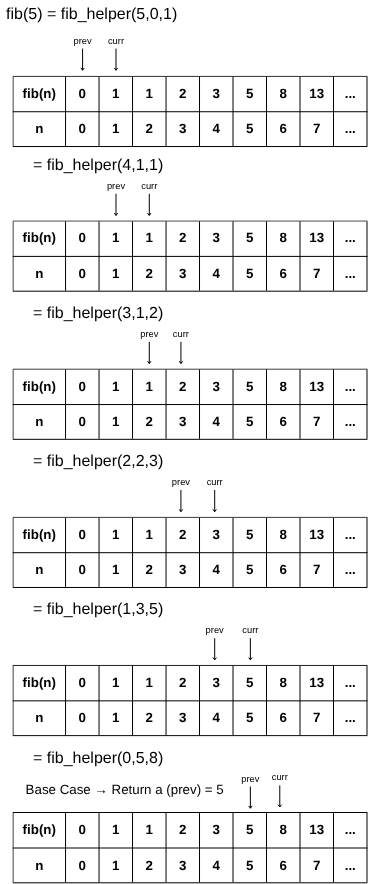
\includegraphics[width=0.3\linewidth]{images/fib_tail_recursion.png}
    \caption{Fib Tail Recursion}
    \label{fig:fib_tail_recursion}
\end{figure}


\section{Peano Arithmetics}

\titledbox{Remember}{
A unary natural number is a term generated by the following grammar rule:

\[
u ::= 0 \mid s(u)
\]

where $0$ denotes zero and $s(u)$ denotes the successor of $u$. Therefore, the set of unary natural numbers is:
\[
\set{0, s(0), s(s(0)), s(s(s(0))), \cdots}
\]
}

\begin{excursion}[Peano Axioms]{}
The following set of axioms are called the Peano axioms. They can be used to \textit{reason} about natural numbers:
\begin{itemize}
    \item \textbf{P1.} $0$ is a unary natural number.
    \item \textbf{P2.} Every unary natural number has a successor that is a unary natural number and that is different from it.
    \item \textbf{P3.} $0$ is not a successor of any unary natural number.
    \item \textbf{P4.} Different unary natural numbers have different successors.
    \item \textbf{P5.} Induction Axiom. Every unary natural number possesses a property $P$ if
    \begin{itemize}
        \item $0$ has the property $P$, and
        \item the successor of every 
        unary natural number that has the property $P$ also possesses property $P$
    \end{itemize}
\end{itemize}
\end{excursion}

\begin{excursion}[Unary Operations]{}
\definition[Addition]{
We define the addition operation inductively:
\begin{itemize}
    \item Adding $0$ to a number does not change it, expressed as: $0 + X = X$.
    \item Adding the successor of $X$ to $Y$ yields the successor of $X + Y$, expressed as: $s(X) + Y = s(X + Y)$.
\end{itemize}
}{}

Similarly, multiplication and exponentiation are defined as follows:
\definition[Multiplication]{
\begin{itemize}
    \item $n \cdot 0 = 0$, and
    \item $n \cdot s(m) = n + (n \cdot m)$
\end{itemize}
}{}

\definition[Exponentiation]{
\begin{itemize}
    \item $n^0 = s(0)$, and
    \item $n^{s(m)} = n \cdot n^m$
\end{itemize}
}{}
\end{excursion}

In Prolog, we can represent unary natural numbers with a predicate \hltext{nat/1} and a functor \hltext{s/1}:

\begin{codeblock}
nat(0).             % 0 is a natural number
nat(s(X)) :- nat(X).  % the successor of a natural number is a natural number
\end{codeblock}

This predicate will return true for all the following:

\begin{codeblock}
nat(0), nat(s(0)), nat(s(s(0))), nat(s(s(s(0)))), ... 
\end{codeblock}

\questionbox{
Can we write unary addition?
}

Let's think about it. This is a \textbf{function} that returns some value given two arguments, so we have to represent that as a $3$-ary predicate.

Suppose we want to do that with a predicate \hltext{add/3}

\begin{codeblock}
add(X,Y,Z)        %true if Z is the result of adding X and Y
\end{codeblock}

Unary addition is recursive. The base case is:

\[
0 + X = X
\]

We simply write:
\begin{codeblock}
add(0,X,X).
\end{codeblock}

The recursive case:

\[
s(X) + Y = s(X + Y)
\]

In Prolog, we declare the third argument (the output) as something of the structure \inlinecode{s(Z)} and in the body we compute that $Z$ as the addition of $X$ and $Y$.

\begin{codeblock}
add(s(X), Y, s(Z)) :- add(X, Y, Z).
\end{codeblock}

Small test ($3 + 2$):

\begin{codeblock}
?- add(s(s(s(0))), s(s(0)), X).
X = s(s(s(s(s(0)))))
\end{codeblock}

\questionbox{
Can we do subtraction?
}

\titledbox{Beauty of Prolog}{
We do not need a separate subtraction predicate! We arranged the arguments in our head to mean addition. We can query the \inlinecode{add/3} predicate itself to have answers for subtractions. Because \inlinecode{add(X, Y, Z)} defines the mathematical relation, subtraction comes for free without writing any new code.
}

\begin{example}{}
We want the result of $3-1=2$. We query our knowledge base to look for the appropriate $X$ such that $X+1=3$:

\begin{codeblock}
?- add(X, s(0), s(s(s(0)))).
X = s(s(0))
\end{codeblock}
\end{example}

Of course, we can define it recursively if we want. Subtraction can be seen as:

\begin{itemize}
    \item $X - 0 = X$ \hfill{Base Case}
    \item $s(X) - s(Y) = X-Y$ \hfill{Recursion}
\end{itemize}

\begin{codeblock}
% Base case: subtracting 0 from any number X leaves X
sub(X, 0, X).

% Recursive step: (X + 1) - (Y + 1) is the same as X - Y
sub(s(X), s(Y), Z) :-
    sub(X, Y, Z).
\end{codeblock}

Small test ($3-1=2$):
\begin{codeblock}
?- sub(s(s(s(0))), s(0), Res).
Res = s(s(0))
\end{codeblock}

And we can define it in terms of addition:

\begin{codeblock}
% sub(A, B, Res) is true if A - B = Res, which means Res + B = A
sub(A, B, Res) :- add(Res, B, A).
\end{codeblock}


Similarly, we can represent unary multiplication:

\[
X \cdot 0 = 0 \qquad X \cdot s(Y) = X + (X \cdot Y)
\]

\titledbox{Sanity Check}{
\[
4 \cdot 3 = 12 \qquad 4 \cdot s(2) = 4 + (4 \cdot 2) = 4 + 8 = 12
\]
}

We write a predicate \inlinecode{mult/3}:

\begin{codeblock}
% Base case
mult(_, 0, 0).

% Recursive step
mult(X, s(Y), Z) :-
    mult(X, Y, W),
    add(X, W, Z).
\end{codeblock}

To see how this works, consider the query computing $2 \times 2 = 4$:
\begin{codeblock}
?- mult(s(s(0)), s(s(0)), Ans).
\end{codeblock}

The execution proceeds by recursively decomposing the second argument down to the base case, and then accumulating the sum on the way back up:

\begin{enumerate}[label=\textbf{Step \arabic*:}, leftmargin=*]
    \item The first call \texttt{mult(s(s(0)), s(s(0)), Ans)} matches the recursive rule with:
    \[
    X = s(s(0)), \quad Y_1 = s(0)
    \]
    To compute the answer, Prolog creates two subgoals:
    \begin{enumerate}[label=(\alph*)]
        \item Compute the sub-product: \texttt{mult(s(s(0)), s(0), $W_1$)}.
        \item Then add: \texttt{add(s(s(0)), $W_1$, Ans)}.
    \end{enumerate}

    \item The second call is the first subgoal \texttt{mult(s(s(0)), s(0), $W_1$)}. This matches the recursive rule again with:
    \[
    X = s(s(0)), \quad Y_2 = 0
    \]
    It generates two further subgoals:
    \begin{enumerate}[label=(\alph*)]
        \item Compute: \texttt{mult(s(s(0)), 0, $W_2$)}.
        \item Then add: \texttt{add(s(s(0)), $W_2$, $W_1$)}.
    \end{enumerate}

    \item Prolog evaluates \texttt{mult(s(s(0)), 0, $W_2$)}. Since the second argument is $0$, it directly matches the \textbf{base case} \inlinecode{mult(_, 0, 0)}, giving:
    \[
    W_2 = 0
    \]

    \item \textbf{Unwinding the Additions:}
    Now the engine resumes and resolves the pending additions back up the call stack:
    \begin{itemize}
        \item \textbf{Resolving $W_1$:} \texttt{add(s(s(0)), 0, $W_1$)} yields:
        \[
        W_1 = s(s(0)) \quad (\text{i.e., } 2 + 0 = 2)
        \]
        \item \textbf{Resolving \texttt{Ans}:} \texttt{add(s(s(0)), s(s(0)), Ans)} yields:
        \[
        \text{Ans} = s(s(s(s(0)))) \quad (\text{i.e., } 2 + 2 = 4)
        \]
    \end{itemize}
\end{enumerate}

All goals succeed, and Prolog returns:
\begin{codeblock}
Ans = s(s(s(s(0))))
\end{codeblock}

\commandnote{
Division comes for free too
}

\begin{example}[Division using Multiplication]{}
Prolog finds $4/2=2$ without writing a division predicate.
\begin{codeblock}
?- mult(s(s(0)), X, s(s(s(s(0))))).
X = s(s(0))
\end{codeblock}
    
\end{example}

Similarly, we can represent unary exponentiation:
\[
X^0 = s(0) \qquad X^{s(Y)} = X \cdot X^Y
\]

\titledbox{Sanity Check}{
\[
3^3 = 3^{s(2)} = 3 \cdot 3^2 = 3 \cdot 9 = 27
\]
}

We write a predicate \inlinecode{uexp/3}:

\begin{codeblock}
% Base case
uexp(_, 0, s(0)).

% Recursive step
uexp(X, s(Y), Z) :-
    uexp(X, Y, W),
    mult(X, W, Z).
\end{codeblock}

Small test ($2^2 = 4$):
\begin{codeblock}
?- uexp(s(s(0)), s(s(0)), Ans).
Ans = s(s(s(s(0))))
\end{codeblock}
\section{Numerical Arithmetic}
To evaluate arithmetic expressions numerically rather than treating them as symbolic data structures, Prolog provides the built-in infix operator \inlinecode{is}.

\begin{example}{}
Notice the crucial difference between the standard unification operator \inlinecode{=} and the arithmetic evaluator \inlinecode{is}:

\begin{codeblock}
?- X = 2 + 3.
X = 2 + 3.

?- X is 2 + 3.
X = 5.
\end{codeblock}

In the first query, \inlinecode{X = 2 + 3} performs purely structural unification; Prolog treats \inlinecode{2 + 3} as the symbolic compound term. 

In the second query, \inlinecode{X is 2 + 3} instructs the engine to compute the numeric value of the right-hand side expression first, and then unify the result with \inlinecode{X}.
\end{example}

\commandnote{
The right-hand side of \inlinecode{is} must be fully instantiated (e.g., X is Y + 1 throws an instantiation error if Y does not already hold a number).
}

Let's write a predicate \inlinecode{fact(X,Y)} that is true if $Y$ is the factorial of $X$. 

For the base case, we know that $0! = 1$.

\begin{codeblock}
fact(0,1).
\end{codeblock}

For the recursive case, we know that $X! = X \cdot (X-1)!$. We write that as follows:

\begin{codeblock}
fact(X,Xfact) :-
    X \= 0,               % \= means not equal
    Y is X-1,
    fact(Y, Yfact), 
    Xfact is X * Yfact.
\end{codeblock}

Quick Test:

\begin{codeblock}
?- fact(0,X).
X = 1
;
false
\end{codeblock}

\begin{codeblock}
?- fact(4,X).
X = 24
;
false
\end{codeblock}

\problembox{
Look at what happens at the bottom of the recursion when Prolog evaluates our query:
\begin{itemize}
    \item Assume the query is just \texttt{?- fact(0,X).}
    \item Prolog matches the first clause.
    \item But the engine sees that there is a second clause in our KB that also matches the query.
    \item Therefore, Prolog creates a Choice point on the stack pointing to clause 2, just in case clause 1 doesn't work out.
    \item This is wasteful: factorial is a deterministic function (there is only one answer), yet Prolog leaves a useless choice point in memory.
\end{itemize}
}

\solutionbox{
The cut operator \inlinecode{!} to the rescue. To fix this, we tell Prolog: \textit{"Once you match the base case, commit to it! Do not leave a choice point, and do not try any other clauses"}
}

\begin{example}[Cut Operator]{}
\begin{codeblock}
fact(0, 1) :- !.
fact(X, Xfact) :-
    X > 0,
    Y is X - 1,
    fact(Y, Yfact),
    Xfact is X * Yfact.
\end{codeblock}

Now if we query:

\begin{codeblock}
?- fact(3, X).
X = 6
\end{codeblock}
\end{example}

\redbox{
Keeping the condition $X > 0$ is important
}

Assume we want to write a predicate \texttt{max(X,Y,Z)} where, given two numbers $X$ and $Y$, $Z$ is their maximum. We can do that as follows:

\begin{codeblock}
max(X, Y, X) :- X >= Y.
max(X, Y, Y) :- X < Y.
\end{codeblock}

Testing.

\begin{codeblock}
?- max(1,2,X).
X = 2

?- max(2,1,X).
X = 2;
false 

?- max(2,2,X).
X = 2;
false
\end{codeblock}

\commandnote{
In the first query, clause 1 tests $1 \geq 2$ and fails immediately, Prolog moves to clause 2 (the last match) and outputs $X=2$ (no backtrack points registered).

In the last two queries, clause 1 tests $2 \geq 1$ or $2 \geq 2$ and succeeds, but Prolog sees that clause 2 is still an untried candidate, so it records a choice point.
}

To solve this, a \textbf{cut} is used:

\begin{codeblock}
max(X, Y, X) :- X >= Y, !.
max(X, Y, Y) :- X < Y.
\end{codeblock}

\begin{codeblock}
?- max(1, 2, X).
X = 2.

?- max(2, 1, X).
X = 2.             

?- max(2, 2, X).
X = 2.             
\end{codeblock}

A programmer might think: \textit{"If $X \geq Y$ was false, then $X < Y$ must be true! Why waste time checking $X < Y$ in clause 2? Let's just omit it!"}:

\begin{codeblock}
max(X, Y, X) :- X >= Y, !.
max(_, Y, Y). 
\end{codeblock}

At first glance, everything seems to work just fine:

\begin{codeblock}
?- max(1, 2, X).
X = 2.

?- max(2, 1, X).
X = 2.             

?- max(2, 2, X).
X = 2.             
\end{codeblock}

But let's try this query:

\begin{codeblock}
?- max(5, 2, 2).
\end{codeblock}

We should get \texttt{false} here but actually we get \texttt{true}!

\begin{itemize}
    \item Prolog tests clause 1 and because $2 \neq 5$ it does not unify, it fails before the cut is ever reached! 
    \item Prolog falls through to clause 2 and it unifies perfectly with the query, that's why we get \texttt{true}.
\end{itemize}

\subsection{Green Cuts vs. Red Cuts}
Cuts are generally classified into two categories based on whether they alter the declarative meaning of the program:
\begin{itemize}
    \item \defemph{Green Cut:} A cut that only improves efficiency. Removing it does not change the set of answers the program produces.
    \item \defemph{Red Cut:} A cut that alters the declarative semantics of the program. Removing it changes the program's output or produces incorrect answers.
\end{itemize}

Assume we have the following program. Children under 18 get a free ticket (0), everyone else pays 10:

\begin{codeblock}
ticket(Age, 0) :- Age < 18, !.
ticket(_, 10).
\end{codeblock}

Let's run a query for a 10-year-old:

\begin{codeblock}
?- ticket(10, Price).
Price = 0.
\end{codeblock}

Everything looks fine. Only one solution: Price = 0.

Now if we delete the cut:
\begin{codeblock}
ticket(Age, 0) :- Age < 18.
ticket(_, 10).
\end{codeblock}

And run the same query:
\begin{codeblock}
?- ticket(10, Price).
Price = 0 ;
Price = 10.
\end{codeblock}

\observationbox{
With the cut, the set of solutions was $\set{\text{Price}=0}$. Without the cut, the set of solutions became $\set{\text{Price}=0, \text{Price}=10}$
}

Because deleting the cut changed the answers and produced an incorrect solution, that cut is a \textbf{red cut}.

If we have a condition in the second clause, then deleting the cut does not produce an incorrect solution, and the purpose of the cut would be just to prune search branches and avoid storing unnecessary backtrack points:

\begin{codeblock}
ticket(Age, 0)  :- Age < 18, !.
ticket(Age, 10) :- Age >= 18.

?- ticket(10, Price).
Price = 0.
\end{codeblock}


\begin{codeblock}
ticket(Age, 0)  :- Age < 18.
ticket(Age, 10) :- Age >= 18.

?- ticket(10, Price).
Price = 0;
false
\end{codeblock}

As we expressed factorial, we can express Fibonacci, where we have two base cases:
\[
\text{fib}(0) = 0 \qquad \text{fib}(1) = 1 
\]

And the recursion:

\[
\text{fib}(X) = \text{fib}(X-1) + \text{fib}(X-2) \quad \forall X. X > 1
\]

\begin{codeblock}
fib(0,0) :- !.
fib(1,1) :- !.
fib(X,Y) :-
    X>1,
    X1 is X-1,
    X2 is X-2,
    fib(X1, X1fib),
    fib(X2, X2fib),
    Y is X1fib + X2fib.
\end{codeblock}

\subsection{Prolog Tail Recursion}

The factorial and Fibonacci predicates we implemented above mimics the head recursion implementation we discussed in Python.

\begin{codeblock}
def factorial(n):
    # Base case
    if n == 0:
        return 1
    # Recursive case
    return n * factorial(n - 1)
\end{codeblock}

\begin{codeblock}
def fibonacci(n):
    # Base cases
    if n == 0:
        return 0
    elif n == 1:
        return 1
    # Recursive case
    return fibonacci(n - 1) + fibonacci(n - 2)
\end{codeblock}

It is more efficient in Prolog to write tail-recursive predicates. Let's try and transform the Python tail-recursive implementation into tail-recursive predicates.

\minititle{Factorial}
\noindent
\begin{minipage}[t]{0.485\textwidth}
\begin{codeblocktitle}[title=\textbf{Prolog}]
fact(X, Y) :-
    fact_helper(X, 1, Y).

fact_helper(0, Acc, Acc) :- !.

fact_helper(X, Acc, Y) :- 
    X > 0, !,
    Prev is X - 1, 
    Z is Acc * X, 
    fact_helper(Prev, Z, Y).
\end{codeblocktitle}
\end{minipage}\hfill
\begin{minipage}[t]{0.485\textwidth}
\begin{codeblocktitle}[title=\textbf{Python Equivalent}]
def fact(n):
    def fact_helper(n, acc):

        if n == 0:
            return acc

        return fact_helper(n - 1, n * acc)
        
    return fact_helper(n, 1)
\end{codeblocktitle}
\end{minipage}

\minititle{Fibonacci}
\noindent
\begin{minipage}[t]{0.485\textwidth}
\begin{codeblocktitle}[title=\textbf{Prolog}]
fib(X,Y) :- 
    fib_helper(X,0,1,Y).

fib_helper(0,Acc,_,Acc) :- !.

fib_helper(X,Acc1,Acc2,Y) :-
    X>0,
    X1 is X - 1,
    Sum is Acc1+Acc2,
    fib_helper(X1, Acc2, Sum, Y).
\end{codeblocktitle}
\end{minipage}\hfill
\begin{minipage}[t]{0.485\textwidth}
\begin{codeblocktitle}[title=\textbf{Python Equivalent}]
def fib(n):
    def fib_helper(n, a, b):

        if n == 0:
            return a

        return fib_helper(n - 1, b, a + b)

    return fib_helper(n, 0, 1)
\end{codeblocktitle}
\end{minipage}

\observationbox{
Notice that in both \texttt{fact\_helper/3} and \texttt{fib\_helper/4}, the recursive call is the \textbf{very last goal} in the clause body. Because no operations remain after it and no choice points are left open, the Prolog engine applies \textbf{Last Call Optimization (LCO)}. It reuses the current stack frame, executing the recursion in $O(1)$ stack space (identical to an imperative \texttt{while} loop)!
}
\section{Lists}
In Prolog, a \textbf{list} is an ordered sequence of elements of arbitrary length. The empty list is represented by the atom \inlinecode{[]}, and any non-empty list is inductively constructed from two parts: a \defemph{Head} (the first element) and a \defemph{Tail} (the list of all remaining elements).

Prolog provides the special bar operator \inlinecode{[H|T]} to destruct and pattern-match lists:

\begin{example}[List Pattern Matching]{ex:list_pattern_matching}
Consider unifying a list with the \inlinecode{[H|T]} pattern:

\begin{codeblock}
?- [H|T] = [1, 2, 3, 4].
H = 1,
T = [2, 3, 4].
\end{codeblock}

Here, Prolog unifies \inlinecode{H} with the first element, and \inlinecode{T} with the sublist of the remaining elements.

Notice what happens with a single-element list:
\begin{codeblock}
?- [H|T] = [apple].
H = apple,
T = [].
\end{codeblock}

\observationbox{
Two critical rules to remember about \inlinecode{[H|T]}:
\begin{itemize}
    \item \inlinecode{H} (the Head) is a \textbf{single element} (which can be a number, atom, variable, or another list).
    \item \inlinecode{T} (the Tail) is \textbf{always a list} (if there are no elements left, \inlinecode{T} is the empty list \inlinecode{[]}).
\end{itemize}
}
\end{example}

Because lists are defined inductively, recursive pattern matching on \inlinecode{[H|T]} allows us to implement a rich variety of powerful operations, ranging from basic searching and numerical aggregations to permutations, sorting, and higher-order list processing.

\titledbox{Tip}{
Working with lists in Prolog is a great exercise for your brain to get used to recursion. In imperative programming, \textbf{loops} are the standard when it comes to lists. In Prolog, you are forced to \textbf{think recursively} since recursion is the only \textit{looping} you can get.
}

\minititle{Membership}
We can write a predicate \texttt{is\_member(X,L)} that is only true if $X$ is in the list $L$.

The base case is when $X$ is the head of the list (or the only element in the list):

\begin{codeblock}
is_member(X,[X|_]).
\end{codeblock}

If $X$ is not the original list head, then it is only a member if it is the head of the tail list (the second element), and if not, then the tail of that list (the third element), and so on...

\begin{codeblock}
is_member(X,[X|_]).
is_member(X,[_|T]):-is_member(X,T).
\end{codeblock}

\minititle{Length}
We define a predicate \texttt{my\_length(L,X)} that is true if $X$ is the length of the list $L$. 
\begin{itemize}
    \item Base Case: The empty list has a length of $0$
    \item Recursion: The non-empty list has the length of its tail list plus one.
\end{itemize}

\begin{codeblock}
my_length([],0).
my_length([_|T],L):-
    my_length(T,TailLength),
    L is TailLength + 1.
\end{codeblock}

\minititle{Elements Summation}
We write a predicate \texttt{sumlist(L,X)} that is true if $X$ is the sum of the elements in $L$.

\begin{itemize}
    \item Base Case: The empty list has no elements, the sum is $0$.
    \item Recursion: The non-empty list has a sum equal to the sum of the tail's elements plus the head.
\end{itemize}

\begin{codeblock}
sumlist([],0).
sumlist([H|T],Res):-
    sumlist(T,TailSum),
    Res is TailSum + H.
\end{codeblock}

\minititle{Sum First $n$ Elements}

\begin{codeblock}
sum_first_x(_,0,0):-!.
sum_first_x([H|T],X,Sum):-
    X1 is X - 1,
    sum_first_x(T,X1,TSum),
    Sum is TSum + H.
\end{codeblock}

\minititle{Sum Last $n$ Elements}

\begin{codeblock}
sum_last_x(_,0,0):-!.
sum_last_x(List, X, Sum):-
    sumlist(List,SumAll),
    my_length(List,Length),
    F is Length - X,
    sum_first_x(List, F, ToSubtract),
    Sum is SumAll - ToSubtract.
\end{codeblock}

\minititle{Get Element at Index $X$}

\begin{codeblock}
get_element(0,[H|_],H):-!.
get_element(X,[_|T],E):-
    X>0,
    X1 is X-1,
    get_element(X1,T,E).
\end{codeblock}

\minititle{Check if Element is the Last One}

\begin{codeblock}
is_last(X,[X]):-!.
is_last(X,[_|T]):-
    is_last(X,T).
\end{codeblock}

\minititle{Maximum Element}
We want to write a predicate \texttt{max\_list(L,X)} that is only true if $X$ is the maximum element in the list $L$. 

We can do that by normal recursion and using the built-in \texttt{max/2} predicate. The base case here is a single-element list (because an empty list has no maximum). The recursive case is finding the maximum of the tail (\texttt{TailMax}) and then taking the maximum of the head(\texttt{H}) and \texttt{TailMax}.

\begin{codeblock}
max_list([X], X):-!.

max_list([H|T], Max) :-
    max_list(T, TailMax),
    Max is max(H, TailMax).
\end{codeblock}

If we do not want to use the built-in predicate, we can use Prolog if-else syntax (comparison):

\begin{codeblock}
max_list([X], X):-!.

max_list([H|T], Max) :-
    max_list(T, TailMax),
    (H >= TailMax -> Max is H ; Max is TailMax).
\end{codeblock}

We can also do this using \textbf{Tail Recursion}! We seed an accumulator with the first element of the list, then walk down the list updating the accumulator whenever we see a larger number.

\begin{codeblock}
% Public wrapper: seed accumulator with H
max_list([H|T], Max) :-
    max_acc(T, H, Max).

% Base case: when list is empty, the accumulator is the final answer
max_acc([], Acc, Acc).

% Case 1: Head is greater than Acc -> update accumulator to H
max_acc([H|T], Acc, Max) :-
    H > Acc, !,
    max_acc(T, H, Max).

% Case 2: Head is smaller or equal -> keep current Acc
max_acc([_|T], Acc, Max) :-
    max_acc(T, Acc, Max).    
\end{codeblock}

\minititle{Concatenation}
We want to write a predicate \texttt{concat(L1, L2, Res)} that is true if \texttt{Res} is the result of concatenating list \texttt{L2} to \texttt{L1}.

\begin{codeblock}
concat([],X,X).
concat([H|T], Y, [H|T1]):-
    concat(T,Y,T1).
\end{codeblock}

\commandnote{
Prolog offers a built-in predicate \texttt{append/3} that does the same thing
}

\minititle{Append Element}

We write a similar predicate where the second argument is an element (not a list):

\begin{codeblock}
append_element([], X, [X]).
append_element([H|T],X,[H|T1]):-
    append_element(T,X,T1).
\end{codeblock}

\minititle{Remove First Occurrence}

We write a predicate \texttt{remove\_one(X,L,R)} that is true if $R$ is the list $L$ where the first occurrence of $X$ is removed. The base case here is when $X$ is the head of the list, then we just want $R$ to be the tail of $L$. The recursive step is when $X$ is not the head $H$, we keep $H$ and alter the tail to be the list where the first occurrence of $X$ is removed.

\begin{codeblock}
remove_one(X,[X|T],T):-!.
remove_one(X,[H|T],[H|T2]):-
    H \= X,
    remove_one(X,T,T2).
\end{codeblock}

\minititle{Remove All Occurrences}

We want to write a similar predicate, but we want to remove all occurrences of the element $X$.

\begin{codeblock}
remove_all(_,[],[]).
remove_all(X,[X|T],Res) :-
    !,
    remove_all(X,T,Res).
remove_all(X,[H|T],[H|T1]):-
    H \= X,
    remove_all(X,T,T1).
\end{codeblock}

\minititle{Remove Duplicates}

We want to write a predicate \texttt{remove\_duplicates(L1, L2)} that is true if \texttt{L2} is a copy of \texttt{L1} with no duplicates. Here, we do not want to remove all occurrences, neither the first occurrence. For each element that appears more than once, we want to keep the first occurrence, and remove all later occurrences.

Since we want to remove all subsequent occurrences, we can use the predicate \texttt{remove\_all/3} we defined earlier.

\begin{codeblock}
remove_duplicates([],[]).
remove_duplicates([H|T], [H|T3]):-
    remove_all(H, T, T2),
    remove_duplicates(T2,T3).
\end{codeblock}

\minititle{Permutations}

We want to write a predicate \texttt{permutations(L1, L2)} that is only true if \texttt{L2} is a possible permuted copy of \texttt{L1}.

Example Query:
\begin{codeblock}
?- permutations([1,2,3],[3,2,1]).
true
\end{codeblock}

Additionally, we want to get all possible permutations via Prolog backtracking if we query with a variable in the second argument.

Example Query:
\begin{codeblock}
?- permutations([1,2,3],X).

X = [1, 2, 3];
X = [2, 1, 3];
X = [2, 3, 1];
X = [1, 3, 2];
X = [3, 1, 2];
X = [3, 2, 1].
\end{codeblock}

Remember our \texttt{remove\_one} predicate:

\begin{codeblock}
?- remove_one(1,[1,2,3],X).
X = [2, 3]
\end{codeblock}

\questionbox{
What if we used it the other way around? We want to provide the element to be removed, the resulted list, and query for the possible original list.
}

\begin{codeblock}
?- remove_one(1,X,[2, 3]).
X = [1, 2, 3]
\end{codeblock}

\problembox{
That is great, but we want backtracking to give us all possible original lists.
}

\ideabox{
Remove the cut from the base case.
}

\begin{codeblock}
remove_one(X,[X|T],T).         %cut removed
remove_one(X,[H|T],[H|T2]):-
    H \= X,
    remove_one(X,T,T2).
\end{codeblock}

Let's try that again:

\begin{codeblock}
?- remove_one(1,X,[2, 3]).

X = [1, 2, 3];
X = [2, 1, 3];
X = [2, 3, 1].
\end{codeblock}

That exactly is what we hoped for! We can use that idea in our permutation predicate!

We can write the base case as permuting an empty list gives us an empty list as well. But what about the recursive step?

\ideabox{
A permutation \texttt{Perm} of a non-empty list \texttt{[H|T]} is actually the result if we do that \texttt{remove\_one} trick to the permuted tail where the element is the head! i.e. it is \texttt{remove\_one(H,Perm,Tperm)} where we get \texttt{Tperm} from \texttt{permutations(T,Tperm)}
}

Let's write this!

\begin{codeblock}
permutations([],[]).
permutations([H|T],Perm):-
    permutations(T,Tperm),
    remove_one(H,Perm,Tperm).
\end{codeblock}

Let's test it:

\begin{codeblock}
permutations([1,2,3],[3,2,1]).
true
\end{codeblock}

\begin{codeblock}
?- permutations([1,2,3],X).

X = [1, 2, 3];
X = [2, 1, 3];
X = [2, 3, 1];
X = [1, 3, 2];
X = [3, 1, 2];
X = [3, 2, 1].
\end{codeblock}


\minititle{Sort}

We want to write a predicate \texttt{sort\_list(L1, L2)} that is only true if \texttt{L2} is the sorted (ascending) version of \texttt{L1} (duplicates are allowed).

\begin{codeblock}
?- sort_list([4,2,6,1,9,2,1,3],X).
X = [1, 1, 2, 2, 3, 4, 6, 9]
\end{codeblock}

\ideabox{
If you think about this, the sorted version is just one of the permutations of the list that is sorted!
}

\ideabox{
Let's first write a predicate that checks if a list is sorted!
}

We write a predicate \texttt{sorted/1}:
\begin{itemize}
    \item The empty list is considered sorted (trivially)
    \item The list with one element is sorted as well (also trivially)
    \item Recursion applies for lists with two or more elements. It will be sorted if the first element is less than or equal the second element and the tail itself (second element included) is sorted!
\end{itemize}

\begin{codeblock}
sorted([]).
sorted([_]).
sorted([H1,H2|T]):- 
    H1=<H2, 
    sorted([H2|T]).
\end{codeblock}

\begin{codeblock}
?- sorted([1,1,2,3,4,4,5]).
true
\end{codeblock}

Now for the \texttt{sort\_list} predicate, the base case is when we have an empty list, we just return an empty list. For the non-empty list, all we have to do is to look for a permutation of the list where that permutation is sorted! Once we find that, we cut!

\begin{codeblock}
sort_list([],[]).
sort_list(X,Y):-
    permutations(X,Y),
    sorted(Y),!. 
\end{codeblock}

\begin{codeblock}
?- sort_list([6,2,4,8,1,3,1],X).
X = [1, 1, 2, 3, 4, 6, 8]
\end{codeblock}

\titledbox{Fun Fact}{
Defining sort as that is the classic \textbf{Permutation Sort} (or Slowsort). It runs in $\bigo{n \cdot n!}$ time which is the purest declarative (yet computationally terrible) sorting algorithm in computer science.
}
\questionbox{
What if we also would like to remove the duplicates?
}

\answerbox{
Well, we just use our \texttt{remove\_duplicates}!
}

\begin{codeblock}
sort_list([],[]).
sort_list(X,Y):-
    permutations(X,Y1),
    sorted(Y1),!,
    remove_duplicates(Y1,Y).
\end{codeblock}

\begin{codeblock}
?- sort_list([9,2,1,8,1,6,19,2,6],X).
X = [1, 2, 6, 8, 9, 19]
\end{codeblock}

\commandnote{
Prolog provides a built-in \texttt{sort/2} predicate that does exactly that.
}



\minititle{Zip}

We want to write a predicate \texttt{zip(L1,L2,L3)} where \texttt{L3} is the result of zipping two lists \texttt{L1} and \texttt{L2}. 

Example Usage:
\begin{codeblock}
?- zip([1,2,3,4], [5,6], X).
X = [(1,5), (2,6)]

?- zip([1,2], [3,4,5], X).
X = [(1,3), (2,4)]
\end{codeblock}

\commandnote{
The resulted list has as many elements as the smaller input list.
}

To make sure we stop the recursion when the smaller list is empty, we make two base cases:
\begin{itemize}
    \item Zipping the empty list with any \texttt{L2} gives us an empty list (\texttt{L1} is smaller)
    \item Zipping any \texttt{L1} with the empty list gives us an empty list (\texttt{L2} is smaller)
\end{itemize}

The recursion step for non-empty lists starts by zipping the two heads together as the first element and the tail is the result of zipping the two tails!

\begin{codeblock}
zip([],_,[]) :- !.
zip(_,[],[]) :- !.
zip([H1|T1], [H2|T2], [(H1, H2)|T3]) :-
    zip(T1, T2, T3).
\end{codeblock}


\minititle{Flatten}

We want to write a predicate \texttt{flatten\_list(L1, L2)} that is true when \texttt{L2} is flattened list of a list of lists \texttt{L1}. 

Example Usage:
\begin{codeblock}
?- flatten_list([[1,2],3,[4,[5,[6,7,[8]]]]],X).
X = [1, 2, 3, 4, 5, 6, 7, 8]
\end{codeblock}

The base case would be flattening an empty list would just give an empty list back. 

For recursion, we have two cases:
\begin{itemize}
    \item The head itself is a list
    \item The head is just an element
\end{itemize}

\commandnote{
To check if something is a list, we can use the Prolog built-in \texttt{is\_list/1}. 
}

If the head is a list, we need to flatten the head first, flatten the tail, and then append those flattened versions together. 

If the head is a single element, we just output a new list with the same head where the tail is flattened!

Putting things together:

\begin{codeblock}
flatten_list([], []).

flatten_list([H|T], Res) :-
    is_list(H), !,
    flatten_list(H, Hflat),
    flatten_list(T, Tflat),
    append(Hflat, Tflat, Res).

flatten_list([H|T], [H|T1]) :-
    flatten_list(T, T1).
\end{codeblock}

\begin{codeblock}
?- flatten_list([[[1,2,3],4,5],[[6]]],X).
X = [1, 2, 3, 4, 5, 6]
\end{codeblock}

\commandnote{
Prolog provides a built-in predicate \texttt{flatten/2} that does that.
}

\minititle{Reverse Order}

We want to write a predicate \texttt{reverse\_order(L1, L2)} that is true if \texttt{L2} contains the elements of \texttt{L1} in reverse order.

\begin{codeblock}
reverse_order([],[]).
reverse_order([H|T],Res):-
    reverse_order(T,TailRev),
    append(TailRev,[H],Res).
\end{codeblock}

\commandnote{
Prolog provides a built-in predicate \texttt{reverse/2} that does the same thing.
}

\minititle{Remove Elements}

We want to write a predicate \texttt{remove\_elements(L1, L2, L3)} that is only true if \texttt{L3} is a copy of \texttt{L1} where all occurrences of elements in \texttt{L2} (and \texttt{L1}) are removed.

Example Usage:
\begin{codeblock}
?- remove_elements([1,2,3,4,3,1,4], [1,3,6],X).
X = [2, 4, 4]
\end{codeblock}

Obviously here we need to check membership, so we will use our \texttt{is\_member/2}:

\begin{codeblock}
is_member(X, [X|_]) :- !.             % Added cut to prevent useless backtrack point
is_member(X, [_|T]) :- is_member(X, T).
\end{codeblock}

For the base case, if we want to remove elements from the empty list, we just give the empty list (no intersection). 

For non-empty lists, we have two recursive cases:
\begin{itemize}
    \item The head of \texttt{L1} is a member of \texttt{L2} $\leadsto$ We discard it and call the predicate on the tail.
    \item The head is not a member $\leadsto$ We keep it and call the predicate on the tail. 
\end{itemize}

\begin{codeblock}
remove_elements([],_, []).

remove_elements([H|T], List, Res) :-
    is_member(H, List), !,
    remove_elements(T, List, Res).

remove_elements([H|T], List, [H|T1]) :-
    remove_elements(T, List, T1).
\end{codeblock}

\begin{codeblock}
?- remove_elements([1,2,3,4,4,3,2,1], [1,3],X).
X = [2, 4, 4, 2]
\end{codeblock}

\minititle{Hide}
\texttt{hide/3} is similar to \texttt{remove\_elements/3}, but instead of removing the elements, we replace them with the constant \texttt{hidden}:

\begin{codeblock}
?- hide([1,2,1,4,3,9], [1,1,9,4], X).
X = [hidden, 2, hidden, hidden, 3, hidden]
\end{codeblock}

The implementation is straightforward:

\begin{codeblock}
hide([],_, []).

hide([H|T], Elements, [hidden|T1]) :-
    is_member(H, Elements), !,
    hide(T, Elements, T1).

hide([H|T], Elements, [H|T1]) :-
    hide(T, Elements, T1).
\end{codeblock}

\subsection{Higher-Order Predicates}
In logic programming, a \textbf{higher-order predicate} (or meta-predicate) is a predicate that takes \textit{other predicates} or goals as arguments, enabling us to treat code as data and write generic, reusable abstractions.

To dynamically invoke a predicate passed as a variable argument, Prolog provides the built-in \inlinecode{call/N} family:
\begin{itemize}
    \item \inlinecode{call(Goal)} executes \inlinecode{Goal} directly.
    \item \inlinecode{call(Pred, Arg1, ..., ArgN)} appends the arguments to \inlinecode{Pred} and invokes the resulting goal. For example, \inlinecode{call(square, 3, Y)} dynamically constructs and executes the query \inlinecode{square(3, Y)}.
\end{itemize}


\minititle{Map}

We want to write a predicate \texttt{map(P, L1, L2)} that is only true if \texttt{L2} contains the elements of \texttt{L1} where predicate \texttt{P} is applied to each of them. 

For example, assume we have a predicate that squares a number $X$:
\begin{codeblock}
square(X,Y) :- Y is X*X.
\end{codeblock}

We want the following behaviour of our \texttt{map/3} if we pass \texttt{square} as the argument \texttt{P}:

\begin{codeblock}
?- map(square, [1,2,3], X).
X = [1, 4, 9]
\end{codeblock}

For the base case, if \texttt{L1} is empty, then \texttt{L2} is empty as well (regardless of what predicate we passed).

If we have a non-empty list \texttt{[H|T]}, we want \texttt{L2} to have \texttt{H2} where \texttt{H2} is the result of \textbf{calling} \texttt{square} on \texttt{H1} (here where we use the built-in \texttt{call/N}). The tail of \texttt{L2} is the result of recursively calling \texttt{map} on the tail \texttt{T} passing the same \texttt{square}.


\begin{codeblock}
map(_,[],[]).

map(P,[H|T],[H1|T1]) :-
    call(P,H,H1),
    map(P,T,T1).
\end{codeblock}

\begin{codeblock}
?- map(square, [4,5], X).
X = [16, 25]
\end{codeblock}

\minititle{Remove If}

We want to write a predicate \texttt{remove\_if(P, L1, L2)} that is true if \texttt{L2} is a copy of \texttt{L1} with all elements for which the predicate \texttt{P} holds removed. Think of this as filtering: for example, filtering out all even elements, all odd elements, and so on.

Assume we have the following \texttt{odd/1} and \texttt{even/1} predicates:

\begin{codeblock}
even(X) :- 0 is X mod 2.

odd(X) :- \+ even(X).
\end{codeblock}

\commandnote{
In Prolog, \texttt{\textbackslash{}+} represents \textbf{Negation as Failure (NAF)}, read as \textit{"not provable"}. The goal \texttt{\textbackslash{}+ Goal} succeeds if \texttt{Goal} fails to be proven from the knowledge base, and fails if \texttt{Goal} succeeds. Thus, \texttt{odd(X)} simply succeeds whenever \texttt{even(X)} fails. This is similar to non-derivability ($\nvdash$) in proof calculi:
\[
\texttt{\textbackslash{}+} A \Leftrightarrow \text{KB}\nvdash A
\]
}

We expect the following behavior from our predicate:

\begin{codeblock}
?- remove_if(even,[1,2,3,4,5,6],X).
X = [1, 3, 5]
\end{codeblock}

If we provide an empty list we just output an empty list (base case). If we have a non-empty list, we have two recursive cases:
\begin{itemize}
    \item The passed predicate holds for the head $\leadsto$ Discard the head and recurse on the tail.
    \item Otherwise, we keep the head and recurse on the tail.
\end{itemize}

\begin{codeblock}
remove_if(_, [], []).

remove_if(Pred, [H|T], Res) :-
    call(Pred, H), !,
    remove_if(Pred, T, Res).

remove_if(Pred, [H|T], [H|T1]) :-
    remove_if(Pred, T, T1).
\end{codeblock}

\begin{codeblock}
?- remove_if(odd,[1,2,3,4,5,6],X).
X = [2, 4, 6]
\end{codeblock}

\begin{excursion}[Alternative Solution]{}
Using if-else syntax instead of two recursive cases:
\begin{codeblock}
remove_if(_, [], []).

remove_if(Pred, [H|T], Res) :-
    (   call(Pred, H)
    ->  remove_if(Pred, T, Res)
    ;   Res = [H|T1],
        remove_if(Pred, T, T1)
    ).
\end{codeblock}
\end{excursion}

\titledbox{Tip}{
Speaking of if-else, instead of scattering \texttt{(-> ;)} everywhere in your code, you can define a reusable higher-order control block using \texttt{call/1}
}

\begin{example}[Reusable Control Structure]{}
\begin{codeblock}
if_then_else(Condition, Then, Else) :-
    (   call(Condition)
    ->  call(Then)
    ;   call(Else)
    ).
\end{codeblock}
\end{example}

Therefore, the alternative solution can be written as:

\begin{codeblock}
remove_if(_, [], []).
remove_if(Pred, [H|T], Res) :-
    if_then_else(
        call(Pred, H),                              
        remove_if(Pred, T, Res),                  
        (Res = [H|T1], remove_if(Pred, T, T1)) 
    ).
\end{codeblock}

\minititle{Pack}
We want to write a predicate \texttt{pack(L1, L2)} that packs similar consecutive elements in \texttt{L1} in a list inside \texttt{L2}. For example:

\begin{codeblock}
?- pack([a,a,a,b,b,a,c,c,c], X).
X = [[a, a, a], [b, b], [a], [c, c, c]]
\end{codeblock}

We have two base cases:
\begin{itemize}
    \item Packing an empty list $\leadsto$ empty list 
    \item Packing a list with one element $\leadsto$ a list containing a single sublist, \texttt{[[X]]}.
\end{itemize}

For lists with two or more elements, we compare the first two adjacent items:
\begin{itemize}
    \item \textbf{The first two elements are the same} $\leadsto$ they belong to the same group. We attach the first element to the front of the ongoing group formed by packing the rest of the list.
    \item \textbf{The first two elements are different} $\leadsto$ the current run has ended. We seal the first element into its own completed group, and begin packing a new group starting from the second element.
\end{itemize}
Putting it all together, we obtain:

\begin{codeblock}
pack([], []) :- !.
pack([X], [[X]]) :- !.
pack([X, X|T], [[X|Xs]|TPacked]) :- !,
    pack([X|T], [Xs|TPacked]).
pack([X, Y|T], [[X]|TPacked]) :-
    pack([Y|T], TPacked).
\end{codeblock}

\minititle{Encode}
We want to write a predicate \texttt{encode(L1, L2)} where consecutive duplicates of elements in \texttt{L1} are compressed into pairs of the form \texttt{[Count, Element]} in \texttt{L2} (known as \textbf{run-length encoding}):

\begin{codeblock}
?- encode([a,a,a,b,b,c,a,a,d,e,e,e,e], X).
X = [[3, a], [2, b], [1, c], [2, a], [1, d], [4, e]]
\end{codeblock}

\ideabox{
We can use our \texttt{pack}!
}

If we call \texttt{pack}, we already get something useful:

\begin{codeblock}
?- pack([a,a,a,b,b,c,a,a,d,e,e,e,e], X).
X = [[a, a, a], [b, b], [c], [a, a], [d], [e, e, e, e]]
\end{codeblock}

\questionbox{
What can we do with this ?
}

\ideabox{
We can create a helper predicate that takes a list of consecutive duplicates and gives us a list with the count and the element. 
}

\begin{codeblock}
to_rle([H|T], [Count, H]) :-
    length([H|T], Count).
\end{codeblock}

\begin{codeblock}
?- to_rle([a,a,a], X).
X = [3, a]
\end{codeblock}

\questionbox{Okay ... What can we do with that?}

\ideabox{Use our \texttt{map/3} to apply that helper to each element of the resulted list from \texttt{pack}!}

\begin{codeblock}
encode(List, Encoded) :-
    pack(List, Packed),
    map(to_rle, Packed, Encoded).
\end{codeblock}

That works just fine!

\begin{codeblock}
?- encode([a,a,b,c,c,c], X).
X = [[2, a], [1, b], [3, c]]
\end{codeblock}

\begin{excursion}[Different Approach]{}
Here is a different implementation for the \texttt{encode/2} predicate.

\begin{codeblock}
% Public wrapper
encode([], []) :- !.
encode([X|Xs], Encoded) :-
    encode_run(Xs, X, 1, Encoded).

% Base case
encode_run([], Prev, Count, [[Count, Prev]]) :- !.

% Case 1: Same element -> increment count and continue
encode_run([X|Xs], X, Count, Encoded) :- !,
    NextCount is Count + 1,
    encode_run(Xs, X, NextCount, Encoded).

% Case 2: New element -> close current run [Count, Prev], start new run at 1
encode_run([X|Xs], Prev, Count, [[Count, Prev]|Rest]) :-
    encode_run(Xs, X, 1, Rest).
\end{codeblock}
\end{excursion}
\section{Fun with Towers of Hanoi}
The Towers of Hanoi is a puzzle that consists of three pegs (\(A\), \(B\), and \(C\)) and a number of disks of different sizes, which can slide onto any peg. The puzzle starts with the disks arranged in a stack in ascending order of size on one peg, with the smallest disk at the top, forming a conical shape.

\begin{figure}[H]
    \centering
    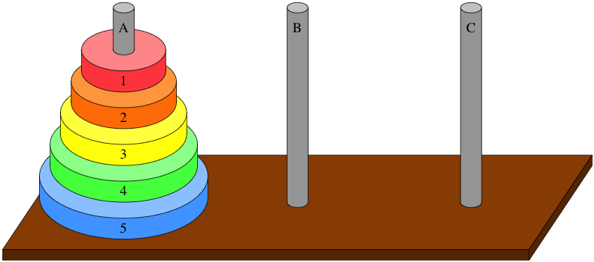
\includegraphics[width=0.4\linewidth]{images/5b5fb2670c9a185b2666637461e40c805fcc9ea5.png}
\end{figure}

The objective of the puzzle is to move all disks from peg \(A\) to peg \(B\) using the auxiliary peg $C$, while obeying the following rules:
\begin{enumerate}
    \item Only one disk may be moved at a time.
    \item Each move consists of taking the upper disk from one of the stacks and placing it on top of another stack or on an empty peg.
    \item No larger disk may be placed on top of a smaller disk.
\end{enumerate}

Here is an illustration of the steps needed to solve the puzzle for three disks:

\begin{figure}[H]
    \centering
    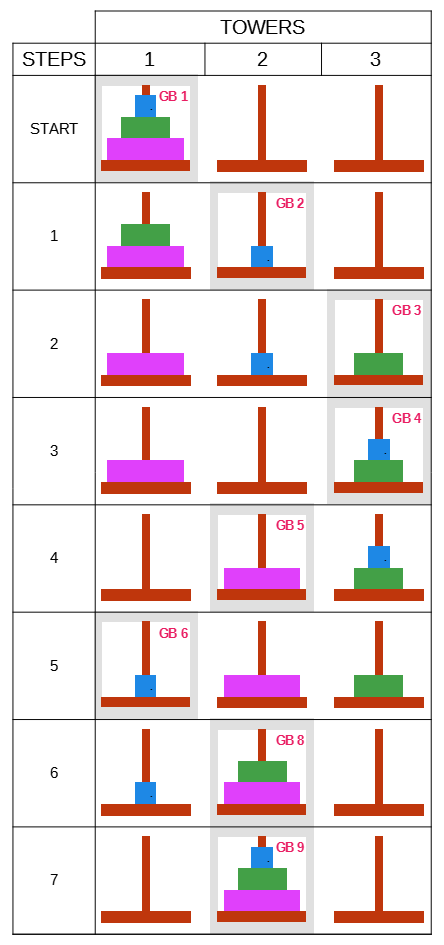
\includegraphics[width=0.3\linewidth]{images/000LCV-2.png}
\end{figure}


We want to write a predicate \texttt{move(N, Source, Target, Aux)} that prints the exact sequence of individual moves required to solve the puzzle for $N$ disks.

\titledbox{Think Recursively}{
If we think about the problem recursively, when we have $N>1$ disks, we want to move the top $N-1$ disks to the auxiliary peg, then move the one biggest disk to the target peg, then move the $N-1$ disks from the auxiliary to the target peg. The base case is trivial: moving one disk requires just a single direct move from source to target!
}

\titledbox{Prolog Printing}{
\begin{itemize}
    \item We will use the \texttt{write(X)} predicate that prints the value of \(X\) (\(X\) can be simple text or any type of argument) to the screen.
    \item We will use \inlinecode{nl} that prints a new line.
\end{itemize}
}

Let's write the base case (one disk):

\begin{codeblock}
move(1, A, B, _) :- !,
    write("Move top disk from "),
    write(A), write(" to "), write(B), nl.
\end{codeblock}

This is what we will get when we call it:

\begin{codeblock}
?- move(1, left,center,right).
Move top disk from left to center
true
\end{codeblock}

The recursion:

\begin{codeblock}
move(N,A,B,C) :-
    N>1,
    N1 is N-1,
    move(N1,A,C,B),
    move(1,A,B,_),
    move(N1,C,B,A).
\end{codeblock}

Let's test this:
\begin{codeblock}
?- move(3, left, center,right).
Move top disk from left to center
Move top disk from left to right
Move top disk from center to right
Move top disk from left to center
Move top disk from right to left
Move top disk from right to center
Move top disk from left to center
true
\end{codeblock}


\newpage
\begin{excursion}[Towers of Hanoi Time Complexity]{}
Let $T(N)$ be the number of moves needed to move $N$ disks. 

If there is only one disk, you move it once (base case):
\[
T(1) = 1
\]

For the recursive case, we want to move $N>1$ disks from peg $A$ to $B$ using $C$:
\begin{enumerate}
    \item Move $N-1$ disks from $A$ to $C$ (\textit{that takes $T(N-1)$ moves})
    \item Move the largest disk from $A$ to $B$ (\textit{one move})
    \item Move the $N-1$ disks from $C$ to $B$ (\textit{another $T(N-1)$ moves})
\end{enumerate}

Therefore:

\[
T(N) = T(N-1) + 1 + T(N-1) = 2T(N-1)+1
\]


Computing $T(N-1)$ the same way gives us 

\[
T(N-1) = T(N-2) + 1 + T(N-2) = 2T(N-2)+1
\]

Substitute:
\[
2T(N-1)+1 = 2(2T(N-2)+1)+1
\]


Expand:

\[
2(2T(N-2)+1)+1 = (4T(N-2) + 2) + 1 = 4T(N-2) + 3
\]

Computing $T(N-2)$ the same way gives us 
\[
T(N-2) = T(N-3) + 1 + T(N-3) = 2T(N-3)+1
\]


Substitute:
\[
4T(N-2) + 3 = 4(2T(N-3)+1) + 3
\]

Expand:
\[
(8T(N-3) + 4) + 3 = 8T(N-3) + 7
\]

And so on $\cdots$


\observationbox{
For a recursive step $k$, we get the following:
\begin{itemize}
    \item $k=1 \to T(N) = 2T(N-1)+1$
    \item $k=2 \to  T(N) = 4T(N-2) + 3$
    \item $k=3 \to T(N) = 8T(N-3) + 7$
\end{itemize}
}


This can be generalized to:

\[
T(N) = 2^k T(N-k) + (2^k - 1)
\]


We stop the recursion when we reach the base case $T(1)$ which occurs when $N-k = 1$ (that is, when $k=N-1$).


For $k = N-1$, we have

\begin{align*}
T(N) &= 2^{N-1} T(N - (N - 1)) + (2^{N-1} - 1) \\
     &= 2^{N-1} T(1) + (2^{N-1} - 1) \\
     &= 2^{N-1} + (2^{N-1} - 1) \\
     &= 2 \cdot 2^{N-1} - 1 \\
     &= 2^N - 1
\end{align*}
\redbox{The complexity is $\mathcal{O}(2^N - 1) = \mathcal{O}(2^N)$, i.e., \textbf{exponential}. For our 3-disk example, $T(3) = 2^3 - 1 = 7$ moves, exactly matching the 7 lines of output above.}
\end{excursion}
\section{Binary Trees}
In Prolog, we do not need special pointers or object classes to represent hierarchical data structures. Instead, we represent a \textbf{binary tree} inductively using compound terms:
\begin{itemize}
    \item \textbf{The empty tree} is represented by the atom \texttt{nil}.
    \item \textbf{A non-empty node} is represented by the 3-ary functor \texttt{tree(Value, Left, Right)}, where \texttt{Value} is the stored item, and \texttt{Left} and \texttt{Right} are themselves binary subtrees.
\end{itemize}
For example, a leaf node containing $1$ is written as \texttt{tree(1, nil, nil)}, while a tree with root $1$ and children $2$ and $3$ is represented as:
\[
\texttt{tree(1, tree(2, nil, nil), tree(3, nil, nil))}
\]
\minititle{Structural Validation: \texttt{is\_b\_tree/1}}
Before performing operations on trees, we want to write a recognizer predicate \texttt{is\_b\_tree(T)} that succeeds if and only if \texttt{T} is a structurally well-formed binary tree.
The inductive definition is straightforward:
\begin{itemize}
    \item \textbf{Base Case:} The empty tree \texttt{nil} is a valid binary tree.
    \item \textbf{Recursive Step:} A compound term \texttt{tree(\_, L, R)} is a valid binary tree if both its left subtree \texttt{L} and right subtree \texttt{R} are valid binary trees.
\end{itemize}
\begin{codeblock}
is_b_tree(nil).
is_b_tree(tree(_, L, R)) :-
    is_b_tree(L),
    is_b_tree(R).
\end{codeblock}
We can verify our representation:
\begin{codeblock}
?- is_b_tree(tree(1, tree(2, nil, nil), tree(3, nil, nil))).
true.
?- is_b_tree(tree(1, invalid_child, nil)).
false.
\end{codeblock}

\minititle{Count Nodes}

We want to count the nodes in a binary tree with the predicate \texttt{bt\_nodes\_count(Tree, Count)}. For the base case, the empty tree has zero nodes. For non-empty trees, the number of nodes is the number of nodes in the left sub-tree added to the number of nodes in the right sub-tree added to one (the root of the tree).

\begin{codeblock}
bt_nodes_count(nil,0):-!.
bt_nodes_count(tree(_, L, R), Res):-
    bt_nodes_count(L,LeftNodes),
    bt_nodes_count(R,RightNodes),
    Res is LeftNodes + RightNodes + 1.
\end{codeblock}

\begin{codeblock}
?- bt_nodes_count(tree(5,tree(3,nil,nil),tree(7,nil,nil)), X).
X = 3
\end{codeblock}

\minititle{Count Leaves}

\texttt{bt\_leaves\_count/2} should count only the leaves of a BT. We have two base cases:
\begin{itemize}
    \item Empty tree $\leadsto$ 0 
    \item A leaf (\texttt{tree(\_,nil,nil)}) $\leadsto$ 1 
\end{itemize}

Otherwise, the sum of the leaves count from the right and left subtrees!

\begin{codeblock}
bt_leaves_count(nil,0):-!.
bt_leaves_count(tree(_,nil,nil),1):-!.
bt_leaves_count(tree(_, L, R), Res):-
    bt_leaves_count(L,LeftLeaves),
    bt_leaves_count(R,RightLeaves),
    Res is LeftLeaves + RightLeaves.
\end{codeblock}

\begin{codeblock}
?- bt_leaves_count(tree(5,tree(3,nil,nil),tree(7,nil,nil)), X).
X = 2
\end{codeblock}

\minititle{Symmetric}
We want to write a predicate \texttt{symmetric/1} that is only true if the binary tree is symmetric. A symmetric BT would look exactly the same if it was mirrored, i.e. flipped horizontally (the subtrees \textbf{mirror} each other).

\begin{figure}[H]
    \centering
    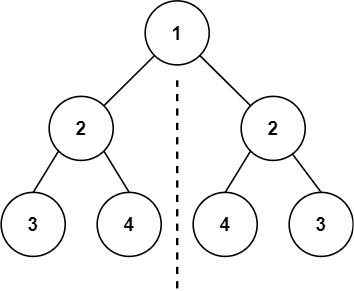
\includegraphics[width=0.3\linewidth]{images/symtree1.jpg}
\end{figure}

\ideabox{
Let's write a helper predicate \texttt{mirror/2} that checks if two BTs mirror each other!
}

The empty tree mirrors itself. For two non-empty trees, they mirror each other if their subtrees do!

\begin{codeblock}
mirror(nil,nil):-!.
mirror(tree(N,L1,R1), tree(N,L2,R2)):-
    mirror(L1,R2),
    mirror(R1,L2).
\end{codeblock}

Let's test that on the subtrees of the image above:

\begin{codeblock}
?- mirror(tree(2, tree(3, nil,nil), tree(4, nil,nil)),
       tree(2, tree(4, nil,nil), tree(3, nil,nil))).
true
\end{codeblock}

\ideabox{
Checking symmetry becomes easier now. The empty tree is symmetric. The non-empty tree is symmetric if its left subtree mirrors its right subtree!
}

\begin{codeblock}
symmetric(nil):-!.
symmetric(tree(_,L,R)):-
    mirror(L,R).
\end{codeblock}

\begin{codeblock}
?- symmetric(tree(1, 
             	tree(2, tree(3, nil,nil), tree(4, nil,nil)),
             	tree(2, tree(4, nil,nil), tree(3, nil,nil))
             )).
true
\end{codeblock}


\minititle{DFS Traversal}
We want to traverse a binary tree using in-order Depth-First Search. This will be straight-forward, we just traverse the left sub-tree, print the root label, and traverse the right sub-tree! 

\begin{codeblock}
bt_dfs_trav(nil):-!.
bt_dfs_trav(tree(N,L,R)):-
    bt_dfs_trav(L),
    write(N), write(" "),
    bt_dfs_trav(R).
\end{codeblock}

\begin{codeblock}
?- bt_dfs_trav(tree(1, 
             	tree(2, tree(3, nil,nil), tree(4, nil,nil)),
             	tree(2, tree(4, nil,nil), tree(3, nil,nil))
             )).

             3 2 4 1 4 2 3
true
\end{codeblock}

\minititle{BFS Traversal}
Breadth-First Search Traversal is a tricky one. We are hoping to print the nodes labels level by level:
\begin{codeblock}
1 2 2 3 4 4 3
\end{codeblock}

\begin{excursion}[Remember BFS]{}
The distinguishing feature of BFS is the use of a \textbf{Queue} operated on a \textbf{FIFO (First-In, First-Out)} basis. Adding newly discovered children to the \textit{back} of the queue guarantees that older sibling nodes waiting at the \textit{front} are processed first.

General Steps:
\begin{enumerate}
    \item \textbf{Initialization:} 
    Create an empty queue $Q$ and enqueue the root node:
    \[
    Q \leftarrow [\text{Root}]
    \]
    \item \textbf{Loop until queue is empty:}
    While $Q$ is not empty:
    \begin{enumerate}[label=(\alph*)]
        \item \textbf{Dequeue:} Remove the node $u$ from the \textbf{front} of $Q$.
        \item \textbf{Visit:} Process node $u$ (e.g., print its value or check a search goal).
        \item \textbf{Enqueue Children:} Add all unvisited children of $u$ to the \textbf{back} of $Q$.
    \end{enumerate}
    \item \textbf{Termination:} 
    When the queue becomes empty, all reachable nodes have been visited.
\end{enumerate}
\end{excursion}

\problembox{
In languages like Python or Java, BFS is straightforward because we can instantiate a mutable \texttt{Queue} object and run a \texttt{while} loop. But in Prolog:
\begin{itemize}
    \item We have \textbf{no \texttt{while} loops}.
    \item We have \textbf{no mutable queue data structures}.
    \item Prolog's execution model is naturally \textbf{Depth-First} (because its execution stack is a LIFO stack!).
\end{itemize}
}

\questionbox{
How do we force a depth-first, immutable language to traverse a tree breadth-first?
}

\titledbox{List-as-Queue Trick}{
The answer lies in passing an explicit \textbf{Queue as a list} across recursive calls:
\begin{enumerate}
    \item \textbf{Popping from the front:} Is just standard list pattern-matching: \inlinecode{[CurrentNode | Rest]}.
    \item \textbf{Pushing to the back:} Is list concatenation using \inlinecode{append/3}:
    \[
    \texttt{append(Rest, [L, R], NewQueue)}
    \]
    By placing children at the \textit{end} of the list, they patiently wait behind all nodes on the current level.
    \item \textbf{The While Loop:} Is replaced by a tail-recursive predicate \texttt{bfs\_loop(Queue)}.
\end{enumerate}
}

\questionbox{
what if a child is \texttt{nil}?
}

\answerbox{
Instead of writing complicated checks before adding children, we simply dump \texttt{[L, R]} onto the queue unconditionally. When a \texttt{nil} eventually bubbles up to the front, a single one-line clause quietly discards it!
}


This entire algorithm boils down to just two clean predicates:
\begin{codeblock}
% 1. Entry Point: Initialize the queue with the root tree
bt_bfs_trav(nil) :- !.
bt_bfs_trav(Tree) :-
    bfs_loop([Tree]).

% 2. The Worker Loop
% Base case: Queue is empty -> traversal finished!
bfs_loop([]) :- !.

% Skip empty branches: When 'nil' reaches the front, discard it!
bfs_loop([nil|Rest]) :- !,
    bfs_loop(Rest).

% Process node: Print value, and enqueue children [L, R] to the back!
bfs_loop([tree(N, L, R)|Rest]) :-
    write(N), write(" "),
    append(Rest, [L, R], NewQueue),
    bfs_loop(NewQueue).
\end{codeblock}

\begin{example}{}
Testing on a balanced binary tree:
\begin{codeblock}
?- Tree = tree(1, 
               tree(2, tree(4, nil, nil), tree(5, nil, nil)), 
               tree(3, tree(6, nil, nil), tree(7, nil, nil))),
   bt_bfs_trav(Tree).
1 2 3 4 5 6 7 
true.
\end{codeblock}
\end{example}



\newpage
\subsection{Binary Search Trees}
While a general binary tree only specifies a hierarchical structure, a \textbf{Binary Search Tree (BST)} enforces a strict \textbf{ordering invariant}:

For every node with value $V$, every element in its \textbf{left subtree} must be strictly smaller than $V$, and every element in its \textbf{right subtree} must be strictly greater than $V$.

This ordering property allows efficient $\mathcal{O}(\log N)$ search, insertion, and retrieval.
\subsubsection*{Node Insertion: \texttt{bst\_ins/3}}
We want to write a predicate \texttt{bst\_ins(Element, OldTree, NewTree)} that inserts an \texttt{Element} into an existing \texttt{OldTree} while preserving the BST ordering invariant, producing \texttt{NewTree}.

There are four distinct cases to consider:
\begin{enumerate}
    \item \textbf{Base Case}: 
    Inserting \texttt{N} into \texttt{nil} yields a new leaf node: \texttt{tree(N, nil, nil)}
    \begin{codeblock}
    bst_ins(N, nil, tree(N, nil, nil)) :- !.
    \end{codeblock}
    \item $N < \text{Root}$:
    The element belongs in the \textbf{left subtree}. We recurse on \texttt{L} to obtain the updated subtree \texttt{Res1}, leaving \texttt{Root} and \texttt{R} unchanged
    \begin{codeblock}
    bst_ins(N, tree(Root, L, R), tree(Root, Res1, R)) :- 
        N < Root, !,
        bst_ins(N, L, Res1).
    \end{codeblock}
    \item $N > \text{Root}$:
    The element belongs in the \textbf{right subtree}. We recurse on \texttt{R} to obtain the updated subtree \texttt{Res1}, leaving \texttt{Root} and \texttt{L} unchanged
    \begin{codeblock}
    bst_ins(N, tree(Root, L, R), tree(Root, L, Res1)) :- 
        N > Root, !,
        bst_ins(N, R, Res1).
    \end{codeblock}
    \item $N = \text{Root}$ (Duplicate element): 
    If the element is already present at the root, we return the tree unchanged
    \begin{codeblock}
    bst_ins(N, tree(N, L, R), tree(N, L, R)) :- !.
    \end{codeblock}
\end{enumerate}

Let's test this, we want to start with the empty tree, insert 5, followed by 3 and 7:
\begin{codeblock}
?- bst_ins(5, nil, T1), bst_ins(3, T1, T2), bst_ins(7, T2, T3).
T1 = tree(5, nil, nil),
T2 = tree(5, tree(3, nil, nil), nil),
T3 = tree(5, tree(3, nil, nil), tree(7, nil, nil)).
\end{codeblock}

\minititle{BST Construction}

\ideabox{
Instead of inserting elements one by one, we want a predicate \texttt{bst\_const/2} that takes a list of elements and gives us the binary search tree consisting of those elements
}

For example, we would like to get the final tree:
\begin{codeblock}
tree(5, tree(3, nil, nil), tree(7, nil, nil))
\end{codeblock}

If we call that predicate with the list \texttt{[7,3,5]} instead of calling the insertion predicate three times:
\begin{codeblock}
bst_ins(5, nil, T1), bst_ins(3, T1, T2), bst_ins(7, T2, T3).
\end{codeblock}

The base case is the empty list, we would just give \texttt{nil} back. For non-empty lists, we construct a BST for the tail, and then insert the head to the result we get.

\begin{codeblock}
bst_const([],nil).
bst_const([H|T], Res):-
    bst_const(T,T1),
    bst_ins(H,T1,Res).
\end{codeblock}

\begin{codeblock}
?- bst_const([7,3,5],X).
X = tree(5,tree(3,nil,nil),tree(7,nil,nil))
\end{codeblock}

\begin{excursion}[Tail Recursive BST Const.]{}
We can instead write a tail-recursive predicate for efficiency. We will insert the elements left to right (starting from the head)

\begin{codeblock}
bst_const(X,Res):- 
    bst_constAcc(X,nil,Res).

bst_constAcc([],Acc,Acc).
bst_constAcc([H|T],Acc,Res):-
    bst_ins(H,Acc,Acc1),
    bst_constAcc(T, Acc1, Res).
\end{codeblock}

\begin{codeblock}
?- bst_const([5,3,7],X).
X = tree(5,tree(3,nil,nil),tree(7,nil,nil))
\end{codeblock}
\end{excursion}
\section{Tree Search Algorithms}

To implement tree search algorithms we need to represent general trees in Prolog (not just binary trees).

\minititle{General Tree}
In binary trees, we always knew that there is a left and right subtrees. But here we do not know how many children a node has.

\begin{example}[Tree Example]{ex:tree1}
\begin{center}
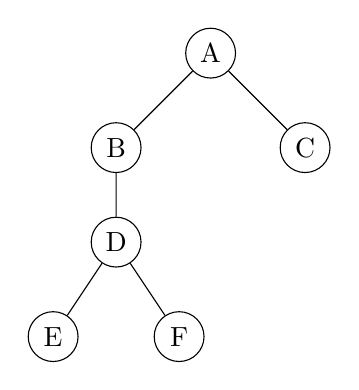
\begin{tikzpicture}[
    level distance=1.2cm,
    level 1/.style={sibling distance=2.4cm},
    level 2/.style={sibling distance=1.6cm},
    level 3/.style={sibling distance=1.6cm},
    every node/.style={vertex}
]
\node {A}
    child { node {B}
        child { node {D}
            child { node {E} }
            child { node {F} }
        }
    }
    child { node {C} };
\end{tikzpicture}
\end{center} 
\end{example}


\begin{example}[Tree Example]{ex:tree2}
\begin{center}
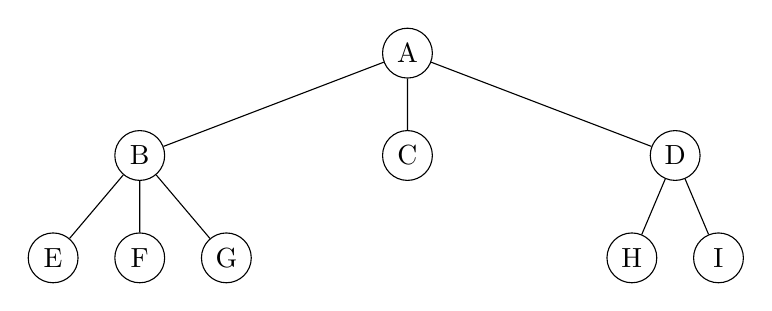
\begin{tikzpicture}[
    level distance=1.3cm,
    level 1/.style={sibling distance=3.4cm},
    level 2/.style={sibling distance=1.1cm},
    every node/.style={vertex}
]
\node {A}
    child { node {B}
        child { node {E} }
        child { node {F} }
        child { node {G} }
    }
    child { node {C} }
    child { node {D}
        child { node {H} }
        child { node {I} }
    };
\end{tikzpicture}
\end{center}
\end{example}

\ideabox{
A tree is a labelled node with a \textbf{list} of children, where each child can itself be a tree (with its own list of children) and leaves are just trees with no children (an empty list of children)
}

We create predicate  \texttt{istree/1} to validate if something is a tree:

\begin{codeblock}
istree(tree(N, Children)):-
    string(N),
    istreelist(Children).

istreelist([]).
istreelist([H|T]):-
    istree(H),
    istreelist(T).
\end{codeblock}

Let's represent the tree in \Exampleref{ex:tree1}

\begin{codeblock}
?- istree(
    tree("A",
         [ tree("B",
                [ tree("D",
                       [ tree("E", []),
                         tree("F", [])
                       ])
                ]),
           tree("C", [])
         ])
  ).
true
\end{codeblock}

And the tree in \Exampleref{ex:tree2}
\begin{codeblock}
?- istree(
    tree("A",
         [ tree("B",
                [ tree("E", []),
                  tree("F", []),
                  tree("G", [])
                ]),
           tree("C", []),
           tree("D",
                [ tree("H", []),
                  tree("I", [])
                ])
         ])
  ).
true
\end{codeblock}

\minititle{DFS}

We want to create a DFS predicate \texttt{dfs/1} that traverses the given tree in a pre-order DFS and prints out the traversed node label along with its depth (level). For example, if we give the tree in \Exampleref{ex:tree2}, we want to get:
\begin{codeblock}
0:A
1:B
2:E
2:F
2:G
1:C
1:D
2:H
2:I
true
\end{codeblock}


\problembox{
\begin{enumerate}
    \item How do we keep track of the current depth level $D$ as we go deeper into the tree?
    \item A node's \texttt{Children} is a \textbf{list} of unknown size. How do we traverse an arbitrary list of trees while maintaining depth-first order?
\end{enumerate}
}

\ideabox{
We want our predicate to be a public wrapper where it initially calls a helper predicate with initial depth of zero.
}

\begin{codeblock}
dfs(T) :- 
    dfsD(T, 0).
\end{codeblock}

\questionbox{
What should \texttt{dfsD/2} do?
}

At any node \texttt{tree(N, Children)} at depth \texttt{D}:
\begin{enumerate}
    \item We first print the current node's label with its depth: \texttt{write(D), write(":"), writeln(N)}.
    \item Its children will live one level deeper: \texttt{Next is D + 1}.
\end{enumerate}

\problembox{
How do we traverse the list of children?
}

\ideabox{
\textbf{The Mutual Recursion Pattern (Trees $\longleftrightarrow$ Lists of Trees):}
\begin{itemize}
    \item A \textbf{tree} contains a list of children.
    \item A \textbf{list of children} contains individual trees.
\end{itemize}
This natural duality calls for \textbf{mutual recursion}: \texttt{dfsD} processes a single tree and delegates the children list to another predicate which walks through the list and calls \texttt{dfsD} on each child tree!
}

Therefore, \texttt{dfsD/2} will look like:
\begin{codeblock}
dfsD(tree(N, Children), D) :-
    write(D), write(":"), writeln(N),
    Next is D + 1,
    dfsAll(Children, Next).
\end{codeblock}

Now, \texttt{dfsAll} simply walks down the list of sibling trees at depth \texttt{D}:
\begin{itemize}
    \item \textbf{Base Case:} An empty list of children \texttt{[]} requires no action.
    \item \textbf{Recursive Step:} Given \texttt{[H|T]}, we process the first child tree \texttt{H} using \texttt{dfsD(H, D)}, and then recursively process the remaining sibling trees \texttt{T} using \texttt{dfsAll(T, D)}.
\end{itemize}

\observationbox{
Notice a subtle but beautiful detail:
\begin{itemize}
    \item When descending from parent to children in \texttt{dfsD}, depth increments: \texttt{Next is D + 1}.
    \item When moving across sibling trees in \texttt{dfsAll}, depth \textbf{remains the same} (\texttt{D}) because all siblings share the exact same level!
\end{itemize}
}

Putting things together:
\begin{codeblock}
% Public wrapper
dfs(T) :- 
    dfsD(T, 0).

% Process a single node: print, increment depth, delegate children
dfsD(tree(N, Children), D) :-
    write(D), write(":"), writeln(N),
    Next is D + 1,
    dfsAll(Children, Next).

% Process a list of sibling trees
dfsAll([], _).
dfsAll([H|T], D) :-
    dfsD(H, D),
    dfsAll(T, D).
\end{codeblock}

Let's run \texttt{dfs/1} on the tree from \Exampleref{ex:tree2}:

\begin{codeblock}
?- dfs(tree("A", [
           tree("B", [tree("E", []), tree("F", []), tree("G", [])]),
           tree("C", []),
           tree("D", [tree("H", []), tree("I", [])])
       ])).
0:A
1:B
2:E
2:F
2:G
1:C
1:D
2:H
2:I
true.
\end{codeblock}


\minititle{BFS}
Similarly, we want to have a predicate \texttt{bfs/1} that traverses the tree in BFS (level by level). We are hoping to get the following output if we call it on the tree in \Exampleref{ex:tree2}:

\begin{codeblock}
0:A
1:B
1:C
1:D
2:E
2:F
2:G
2:H
2:I
true
\end{codeblock}

\newpage
\problembox{
In our depth-first traversal, Prolog did all the heavy lifting: its internal resolution engine naturally behaves like a LIFO stack. Descending into children was as simple as making a recursive call. 

As we discussed earlier, BFS runs in direct opposition to Prolog's execution strategy! If we discover a node's children and immediately make recursive calls on them, Prolog will dive straight down the first child's subtree—collapsing back into DFS. 

To explore nodes level by level, newly discovered children are not allowed to be visited right away. They must wait behind all previously discovered nodes. We need an explicit \textbf{FIFO (First-In, First-Out) queue}, traditionally called an \defemph{exploration fringe}.
}

\questionbox{
If our queue simply holds a list of trees waiting to be explored, say $[T_1, T_2, \dots]$, how will we know the depth of a node when we eventually pop it from the queue?
}

\commandnote{
Notice that at any intermediate stage, the queue might hold sibling nodes from depth $1$ alongside newly enqueued children from depth $2$. A single global counter or depth parameter passed to a recursive loop cannot work, because elements currently waiting in the queue belong to different depths!
}

\ideabox{
We must \textbf{bundle each tree together with its own depth}! 

Instead of storing bare tree terms in the queue, every element in our fringe will be an explicit pair:
\[
(D,\, T)
\]
where $D \in \mathbb{N}$ records the exact depth of subtree $T$. When search begins at the root, the queue starts with just a single pair:
\[
[(0,\, \text{Root})]
\]
}

Let us examine what a single step of breadth-first exploration looks like. Suppose our fringe is non-empty, with the first pair waiting at the front:
\[
[(D,\, \text{tree}(N,\, \text{Children})) \mid \text{ToExplore}]
\]
What actions must take place?
\begin{enumerate}
    \item \textbf{Visit:} Dequeue the front pair and print its depth and label: $D:N$.
    \item \textbf{Calculate Child Depth:} Since this node sits at depth $D$, all of its immediate children belong to depth $D + 1$.
    \item \textbf{Tag Descendants:} Take the raw list of child trees and pair every single one of them with this new depth $D + 1$.
    \item \textbf{Enqueue at the Back:} To preserve the FIFO discipline, add these newly tagged pairs to the \textbf{end} of the remaining queue ($\text{ToExplore}$).
    \item \textbf{Recurse:} Continue exploring the updated queue.
\end{enumerate}
When the queue eventually becomes empty (\texttt{[]}), every reachable node across all levels has been visited, and the process cleanly terminates.

\questionbox{
Before we assemble the main loop, we need a small helper to handle step (3). 

Given a depth $D$ and a list of child trees $[C_1, C_2, \dots, C_k]$, how do we construct a list of pairs $[(D, C_1), (D, C_2), \dots, (D, C_k)]$ in Prolog?
}

\solutionbox{
We define a pairing relation by structural induction on the list of children:
\begin{itemize}
    \item \textbf{Base Case:} Pairing any depth with an empty list of children yields an empty list.
    \item \textbf{Recursive Step:} Given a head child $H$ and tail $T$, we construct the pair $(D, H)$ at the front, and recursively pair $D$ with the remaining tail $T$.
\end{itemize}
}

In Prolog, this translates directly to:

\begin{codeblock}
pair(_, [], []).
pair(D, [H|T], [(D, H)|T2]) :-
    pair(D, T, T2).
\end{codeblock}

With this helper ready, we can formulate our fringe exploration loop:
\begin{itemize}
    \item \textbf{Base Case:} An empty fringe requires no work:
\begin{codeblock}
bfsFringe([]).
\end{codeblock}
    \item \textbf{Recursive Step:} Pull the front pair, print it, compute \texttt{Next is D + 1}, tag the children with \texttt{pair/3}, append them to the end of the existing queue, and recurse:
\begin{codeblock}
bfsFringe([(D, tree(N, Children)) | ToExplore]) :-
    write(D), write(":"), writeln(N),
    Next is D + 1,
    pair(Next, Children, NextToExplore),
    append(ToExplore, NextToExplore, NewFringe),
    bfsFringe(NewFringe).
\end{codeblock}
\end{itemize}

Finally, our \texttt{bfs/1} is just a wrapper that starts the fringe with the root at depth $0$:

\begin{codeblock}
bfs(T) :-
    bfsFringe([(0, T)]).
\end{codeblock}

Putting all the pieces together gives our complete breadth-first engine:

\begin{codeblock}
% wrapper
bfs(T) :-
    bfsFringe([(0, T)]).

% loop
% Base case: empty queue terminates
bfsFringe([]).

% Recursive step: pop front, print, tag children, append to back
bfsFringe([(D, tree(N, Children)) | ToExplore]) :-
    write(D), write(":"), writeln(N),
    Next is D + 1,
    pair(Next, Children, NextToExplore),
    append(ToExplore, NextToExplore, NewFringe),
    bfsFringe(NewFringe).

% Helper: tag each child tree with depth D
pair(_, [], []).
pair(D, [H|T], [(D, H)|T2]) :-
    pair(D, T, T2).
\end{codeblock}

\begin{example}[BFS Queue Evolution Trace]{ex:bfstrace}
To see the FIFO queue in action, let us trace how the fringe evolves when calling \texttt{bfs/1} on the tree from \Exampleref{ex:tree2}:
\begin{itemize}
    \item \textbf{Step 0:} Fringe is $[(0, A)]$. Pop $A$, print \texttt{0:A}. Tag children $B, C, D$ with depth $1$ and enqueue them.
    \item \textbf{Step 1:} Fringe is $[(1, B), (1, C), (1, D)]$. Pop $B$, print \texttt{1:B}. Tag children $E, F, G$ with depth $2$ and append them to the back:
    \[
    [(1, C),\, (1, D),\, (2, E),\, (2, F),\, (2, G)]
    \]
    Notice that $C$ and $D$ remain in front of $E, F, G$!
    \item \textbf{Steps 2--3:} Pop and print \texttt{1:C} and \texttt{1:D}. Enqueue $D$'s children $H, I$ at depth $2$.
    \item \textbf{Remaining Steps:} The queue now contains only depth $2$ nodes: $[(2, E), (2, F), (2, G), (2, H), (2, I)]$, which are dequeued and printed in strict order.
\end{itemize}
\end{example}

Let's traverse the tree in \Exampleref{ex:tree1}:

\begin{codeblock}
?- bfs(tree("A",
         [ tree("B",
                [ tree("D",
                       [ tree("E", []),
                         tree("F", [])
                       ])
                ]),
           tree("C", [])
         ])).
0:A
1:B
1:C
2:D
3:E
3:F
true
\end{codeblock}

\minititle{DLS}
Depth-Limited Search is a DFS but with a cut-off depth limit. We want to write a predicate \texttt{dls(T,L)} that performs DLS traversal of the tree $T$ where $L$ is the cut-off depth limit.

Example usage on the tree in \Exampleref{ex:tree1} with depth limit $=2$:
\begin{codeblock}
?- dls(tree("A",
         [ tree("B",
                [ tree("D",
                       [ tree("E", []),
                         tree("F", [])
                       ])
                ]),
           tree("C", [])
         ]),2).

0:A
1:B
2:D
1:C
true
\end{codeblock}



\questionbox{
Think back to our standard DFS implementation. We used mutual recursion between a single-node processor and a list-of-children processor, carrying an accumulator $D$ for the current depth:
\begin{itemize}
    \item How do we inform our search of the limit $L$?
    \item When the search arrives at a node whose depth satisfies $D > L$, what should happen?
\end{itemize}
}

\ideabox{
We must enforce a \textbf{guard condition}:
\begin{itemize}
    \item If $D > L$, we have overstepped our allowed horizon. The search must immediately succeed vacuously without printing the node or expanding its children.
    \item If $D \le L$, we proceed normally: print the node, increment the depth to $D + 1$, and explore its children under the same ceiling $L$.
\end{itemize}
}

\questionbox{
In Prolog, how do we express: "if $D > L$, stop and do nothing, and \textbf{never} attempt to fall through to the printing clause"?
}

We create a predicate \texttt{dfsUpTo}:

\begin{codeblock}
dfsUpTo(_, D, L) :- 
    D > L, 
    !.
\end{codeblock}

If $D > L$ succeeds, the cut \texttt{!} commits immediately to this clause and burns any choice point that would otherwise attempt the subsequent clauses. Because the body ends right there, it succeeds quietly without printing anything or touching the children.

When $D \le L$, we want to print the current node, compute the children's depth, and pass the list of children together with the next depth and \texttt{L} to our list processor. For that, we create the following predicate:

\begin{codeblock}
dfsUpTo(tree(N, Children), D, L) :- 
    write(D), write(":"), writeln(N), 
    Next is D + 1, 
    dfsUpToAll(Children, Next, L).
\end{codeblock}

The companion list processor simply distributes this logic across all siblings at depth $D$:
\begin{itemize}
    \item \textbf{Base Case:} An empty list of children requires no actions:
\begin{codeblock}
dfsUpToAll([], _, _).
\end{codeblock}
    \item \textbf{Recursive Step:} Explore the head child, then recursively process the remaining siblings:
\begin{codeblock}
dfsUpToAll([H|T], D, L) :- 
    dfsUpTo(H, D, L),
    dfsUpToAll(T, D, L).
\end{codeblock}
\end{itemize}

Finally, our public predicate simply receives the tree $T$ and the cut-off limit $L$, initializing the search at the root level $D = 0$:

\begin{codeblock}
dls(T, L) :- 
    dfsUpTo(T, 0, L).
\end{codeblock}

Putting all the pieces together gives our complete Depth-Limited Search engine:

\begin{codeblock}
% Wrapper: start DLS at depth 0 with limit L
dls(T, L) :- 
    dfsUpTo(T, 0, L).

% Cutoff clause: if depth exceeds limit, prune branch
dfsUpTo(_, D, L) :- 
    D > L, 
    !.

% Expansion clause: visit node, increment depth, recurse into children
dfsUpTo(tree(N, Children), D, L) :- 
    write(D), write(":"), writeln(N), 
    Next is D + 1, 
    dfsUpToAll(Children, Next, L).

% Process list of siblings: base case
dfsUpToAll([], _, _).

% Process list of siblings: recursive step
dfsUpToAll([H|T], D, L) :- 
    dfsUpTo(H, D, L),
    dfsUpToAll(T, D, L).
\end{codeblock}

Let us test \texttt{dls/2} on the tree from \Exampleref{ex:tree2} with different depth limits $L$.

Setting $L = 1$ cuts off all children at depth $2$ ($E, F, G, H, I$):

\begin{codeblock}
?- dls(tree("A", [
           tree("B", [tree("E", []), tree("F", []), tree("G", [])]),
           tree("C", []),
           tree("D", [tree("H", []), tree("I", [])])
       ]), 1).
0:A
1:B
1:C
1:D
true.
\end{codeblock}

If we set $L = 0$, only the root is visited:

\begin{codeblock}
?- dls(tree("A", [
           tree("B", [tree("E", []), tree("F", []), tree("G", [])]),
           tree("C", []),
           tree("D", [tree("H", []), tree("I", [])])
       ]), 0).
0:A
true.
\end{codeblock}

\commandnote{
Setting $L = 2$ allows the search to reach the full depth, reproducing the complete DFS traversal.
}




\minititle{IDS}
Iterative Deepening Search is a DLS with an increasing depth limit. We want a predicate \texttt{ids/1} that traverses the tree starting with a depth limit $0$ and increasing until the maximum actual depth of the tree. For each depth limit, we want to print that depth limit and then traverse the nodes as usual.

Here is what we hope for if we give the tree in \Exampleref{ex:tree1}
\begin{codeblock}
?- ids(tree("A",
         [ tree("B",
                [ tree("D",
                       [ tree("E", []),
                         tree("F", [])
                       ])
                ]),
           tree("C", [])
         ])).

LIMIT = 0
0:A
LIMIT = 1
0:A
1:B
1:C
LIMIT = 2
0:A
1:B
2:D
1:C
LIMIT = 3
0:A
1:B
2:D
3:E
3:F
1:C
true
\end{codeblock}

\ideabox{
Just call DLS with increasing depth limits starting from 0.
}

\problembox{
We want to know when to stop. Because for a finite tree (such as \Exampleref{ex:tree1}, which has a maximum depth of $3$) once we run DLS with $L = 3$, the entire tree has already been completely explored. If we naively continue with $L = 4, 5, 6, \dots$, it would endlessly re-traverse the exact same tree! 
}

\ideabox{
We want some way of reporting back to the outer lopp that the entire tree was explored
}


\ideabox{
We can equip our depth-limited traversal with a \textbf{termination flag}:
\[
\text{Done} \in \{0,\, 1\}
\]
\begin{itemize}
    \item If at \textbf{any} point during the traversal a node exceeds the depth limit ($D > L$), that branch was cut off. Thus, the tree was \textit{not} fully explored, so we report $\text{Done} = 0$.
    \item If a node is a leaf (empty children list \texttt{[]}), it has no children to cut off, so that branch is fully explored: $\text{Done} = 1$.
    \item For an internal node with multiple children, the entire subtree is fully explored if and only if \textbf{all} of its children are fully explored! In arithmetic, a logical $\text{AND}$ over binary flags is simply multiplication:
    \[
    \text{Done} = \text{Done}_H \times \text{Done}_T
    \]
    If even a single child was truncated (returning $0$), the product collapses to $0$!
\end{itemize}
}

Let us refine our depth-limited traversal to carry this fourth argument, reflecting our three cases:

\begin{enumerate}
    \item \textbf{Cutoff Hit ($D > L$):} When the depth ceiling is breached, we prune the branch with a cut (\texttt{!}) and unify the status flag with $0$:
\begin{codeblock}
dfsUpTo(_, D, L, 0) :-
    D > L,
    !.
\end{codeblock}

    \item \textbf{Node Expansion ($D \le L$):} When within limits, we print the node, increment the depth, and let the list of children determine the overall \texttt{Done} status:
\begin{codeblock}
dfsUpTo(tree(N, Children), D, L, Done) :-
    write(D), write(":"), writeln(N),
    D1 is D + 1,
    dfsUpToAll(Children, D1, L, Done).
\end{codeblock}

    \item \textbf{Children Exploration:} An empty list of children represents an exhausted branch ($\text{Done} = 1$). A non-empty list computes the conjunction of all child flags via multiplication:
\begin{codeblock}
dfsUpToAll([], _, _, 1).
dfsUpToAll([H|T], D, L, Done) :-
    dfsUpTo(H, D, L, DoneH),
    dfsUpToAll(T, D, L, DoneT),
    Done is DoneH * DoneT.
\end{codeblock}
\end{enumerate}

\questionbox{
Now that our traversal returns $\text{Done} \in \{0, 1\}$, how do we structure the outer deepening loop?
}

\solutionbox{
At each stage with current limit $C$:
\begin{enumerate}
    \item Print \texttt{LIMIT = C}.
    \item Launch the traversal: \texttt{dfsUpTo(T, 0, C, Done)}.
    \item Inspect the result using a helper predicate:
    \begin{itemize}
        \item If $\text{Done} = 1$, the entire tree was explored without hitting any limit ceiling. Search is complete!
        \item If $\text{Done} = 0$, at least one branch was truncated. Increment the limit to $C + 1$ and recurse!
    \end{itemize}
\end{enumerate}
}

In Prolog, this logic is expressed declaratively with two clauses:

\begin{codeblock}
% Base case: entire tree explored without cutoffs -> stop!
handleDone(_, _, 1).

% Recursive step: cutoff occurred -> increment limit and repeat
handleDone(T, C, 0) :-
    C1 is C + 1,
    idsUntilDone(T, C1).
\end{codeblock}

Our looping predicate ties everything together:

\begin{codeblock}
idsUntilDone(T, C) :-
    write('LIMIT = '), writeln(C),
    dfsUpTo(T, 0, C, Done),
    handleDone(T, C, Done).
\end{codeblock}

Finally, the public entry point starts the iterative deepening process with limit $0$:

\begin{codeblock}
ids(T) :- 
    idsUntilDone(T, 0).
\end{codeblock}

Putting all the components together gives our complete Iterative Deepening Search engine:

\begin{codeblock}
% Wrapper: start IDS at limit 0
ids(T) :- 
    idsUntilDone(T, 0).

% Outer loop
idsUntilDone(T, C) :-
    write('LIMIT = '), writeln(C),
    dfsUpTo(T, 0, C, Done),
    handleDone(T, C, Done).

% Done = 1 -> fully explored, stop
handleDone(_, _, 1).

% Done = 0 -> branch cut off, deepen limit
handleDone(T, C, 0) :-
    C1 is C + 1,
    idsUntilDone(T, C1).

% depth exceeded -> branch truncated (Done = 0)
dfsUpTo(_, D, L, 0) :-
    D > L,
    !.

% visit node, delegate Done status to children
dfsUpTo(tree(N, Children), D, L, Done) :-
    write(D), write(":"), writeln(N),
    D1 is D + 1,
    dfsUpToAll(Children, D1, L, Done).

% no children -> fully explored (Done = 1)
dfsUpToAll([], _, _, 1).

% Done is logical AND of all child statuses
dfsUpToAll([H|T], D, L, Done) :-
    dfsUpTo(H, D, L, DoneH),
    dfsUpToAll(T, D, L, DoneT),
    Done is DoneH * DoneT.
\end{codeblock}

\section{MiniMax}
Minimax is an adversarial search algorithm where the agent competes against an opponent whose goals directly conflict with its own.

We consider \textbf{two-player, zero-sum games of perfect information}:
\begin{itemize}
    \item \textbf{MAX} (Player $+1$): seeks to maximize the terminal game utility.
    \item \textbf{MIN} (Player $-1$): seeks to minimize the terminal game utility.
\end{itemize}

Assuming both players play with perfect rationality, the game-theoretic value $V(s)$ of any state $s$ is governed by the \defemph{Minimax equation}:
\[
V(s) = \begin{cases}
\text{Utility}(s) & \text{if } s \text{ is a terminal state,} \\
\max_{s' \in \text{Children}(s)} V(s') & \text{if it is MAX's turn to move,} \\
\min_{s' \in \text{Children}(s)} V(s') & \text{if it is MIN's turn to move.}
\end{cases}
\]

To make this concrete, we implement an ancient mathematical game: the \defemph{Subtraction Game} (a single-heap variant of Nim):
\begin{itemize}
    \item A pile contains $N$ matches.
    \item Two players alternate turns. On their turn, a player must remove $1$, $2$, or $3$ matches from the pile (provided enough matches remain).
    \item A player who faces an empty pile ($N = 0$) has no legal moves and \textbf{loses}. Equivalently, the player who removes the last match wins!
\end{itemize}

\ideabox{
\textbf{State Representation:} We represent the board state as a compound term:
\[
\texttt{state}(N,\, P)
\]
where $N \in \mathbb{N}$ denotes the number of remaining matches, and $P \in \{1,\, -1\}$ denotes the active player whose turn it is. 
}

\commandnote{
Switching turns is simply arithmetic negation.
}

\minititle{Step 1: Generating Successor States}

From a state $\texttt{state}(N, P)$, what moves are legally available?
\begin{itemize}
    \item If $N \ge 1$, the player can remove $1$ match, leaving $N - 1$ matches for player $-P$.
    \item If $N \ge 2$, the player can remove $2$ matches, leaving $N - 2$ matches for player $-P$.
    \item If $N \ge 3$, the player can remove $3$ matches, leaving $N - 3$ matches for player $-P$.
\end{itemize}
When $N = 0$, no matches remain, and no legal transitions exist.


In Prolog, we represent these non-deterministic possibilities with three distinct clauses:

\begin{codeblock}
% Remove 1 match
successor(state(N, P), NextS) :-
    N > 0,
    N2 is N - 1,
    P2 is -P,
    NextS = state(N2, P2).

% Remove 2 matches
successor(state(N, P), NextS) :-
    N > 1,
    N2 is N - 2,
    P2 is -P,
    NextS = state(N2, P2).

% Remove 3 matches
successor(state(N, P), NextS) :-
    N > 2,
    N2 is N - 3,
    P2 is -P,
    NextS = state(N2, P2).
\end{codeblock}

\minititle{Step 2: Collecting All Legal Moves}
To compute $\max$ or $\min$, our search needs the \textbf{complete list} of all valid child states originating from the current state.

\questionbox{
How can we collect all non-deterministic solutions of \texttt{successor/2} into a single Prolog list?
}

\solutionbox{
We use an accumulator pattern coupled with negation-as-failure:
\begin{itemize}
    \item \textbf{Recursive Step:} Generate a successor \texttt{NextS} using \texttt{successor(S, NextS)}. Check that it has not already been added to our accumulator: \texttt{\textbackslash+ is\_member(NextS, Acc)}. Prepend it to the accumulator and recurse. We cut to commit to collecting all remaining successors.
    \item \textbf{Base Case:} When no new unvisited successors can be generated, the accumulator holds the complete set of moves.
\end{itemize}
}

\begin{codeblock}
successors(S, Acc, NextSs) :-
    successor(S, NextS),
    \+ is_member(NextS, Acc),
    successors(S, [NextS|Acc], NextSs),
    !.
successors(_, Acc, Acc).
\end{codeblock}

\minititle{Step 3: Finding Extremes (Min and Max)}

\questionbox{
Once MAX (or MIN) obtains the list of reachable child states, how do they determine the optimal value?
}

\ideabox{
We fold over the list of child states while maintaining an accumulator for the best utility seen so far:
\begin{itemize}
    \item \textbf{MAX's perspective (\texttt{maxvalue/3}):} For each child state, compute its Minimax value. If the child's value is greater than or equal to the current maximum, update the running maximum.
    \item \textbf{MIN's perspective (\texttt{minvalue/3}):} For each child state, compute its Minimax value. If the child's value is strictly less than the current minimum, update the running minimum.
\end{itemize}
}

Here are the dual fold predicates:

\begin{codeblock}
% maxvalue/3: Find the maximum value among child states
maxvalue([], BestSoFar, BestSoFar).

maxvalue([State|Rest], BestSoFar, Result) :-
    value(State, ChildValue),
    ChildValue >= BestSoFar,
    maxvalue(Rest, ChildValue, Result).

maxvalue([State|Rest], BestSoFar, Result) :-
    value(State, ChildValue),
    ChildValue < BestSoFar,
    maxvalue(Rest, BestSoFar, Result).

% minvalue/3: Find the minimum value among child states
minvalue([], BestSoFar, BestSoFar).

minvalue([State|Rest], BestSoFar, Result) :-
    value(State, ChildValue),
    ChildValue < BestSoFar,
    minvalue(Rest, ChildValue, Result).

minvalue([State|Rest], BestSoFar, Result) :-
    value(State, ChildValue),
    ChildValue >= BestSoFar,
    minvalue(Rest, BestSoFar, Result).
\end{codeblock}

\minititle{Step 4: The Minimax Engine and Terminal States}

Now we tie everything together in our main evaluation predicate:
\begin{itemize}
    \item If it is \textbf{MAX's turn} ($P = 1$): collect all child states, and find the maximum starting from the worst-case utility $-1$.
    \item If it is \textbf{MIN's turn} ($P = -1$): collect all child states, and find the minimum starting from the worst-case utility $+1$.
\end{itemize}

\begin{codeblock}
value(State, Value) :-
    State = state(_, Player),
    Player = 1,
    successors(State, [], ChildStates),
    maxvalue(ChildStates, -1, Value).

value(State, Value) :-
    State = state(_, Player),
    Player = -1,
    successors(State, [], ChildStates),
    minvalue(ChildStates, 1, Value).
\end{codeblock}

\observationbox{
Suppose we reach a terminal state with no matches left:
\begin{itemize}
    \item \textbf{State $\texttt{state}(0, 1)$:} It is MAX's turn, but $N = 0$. \texttt{successors/3} generates an empty list $\texttt{ChildStates} = []$. Then \texttt{maxvalue([], -1, Value)} immediately unifies \texttt{Value = -1}! MAX has no legal moves and therefore loses.
    \item \textbf{State $\texttt{state}(0, -1)$:} It is MIN's turn, but $N = 0$. \texttt{ChildStates} is empty. Then \texttt{minvalue([], 1, Value)} unifies \texttt{Value = 1}! MIN has no legal moves and loses, meaning MAX wins!
\end{itemize}
}

\newpage
\begin{example}{ex:nimtrace}
Let us query \texttt{value/2} for various starting pile sizes with Player $1$ (MAX) moving first:

\begin{codeblock}
?- value(state(1, 1), V).
V = 1.

?- value(state(2, 1), V).
V = 1.

?- value(state(3, 1), V).
V = 1.

?- value(state(4, 1), V).
V = -1.
\end{codeblock}

\textbf{Mathematical Explanation:}
\begin{itemize}
    \item For $N \in \{1, 2, 3\}$, MAX can immediately take all remaining matches, reducing the pile to $0$ and leaving MIN with no moves ($V = 1$).
    \item For $N = 4$, whatever move MAX chooses ($1, 2,$ or $3$), MIN is left with $3, 2,$ or $1$ matches and can take the rest to win on the very next turn! Thus, $N = 4$ is a guaranteed losing state for the first player ($V = -1$).
\end{itemize}
In general, for any subtraction game with moves $\{1, 2, 3\}$, a position is a losing position for the current player if and only if:
\[
N \equiv 0 \pmod 4
\]
Our Minimax implementation discovers this exact mathematical truth automatically through search!
\end{example}
\section{Fun with Propositional Logic}

A propositional well-formed formula (WFF) is defined inductively over a signature of variable symbols $\mathcal{V}$ and logical connectives $\{\neg, \wedge, \vee, \to\}$:
\begin{itemize}
    \item Every propositional variable $p \in \mathcal{V}$ is a formula.
    \item If $\varphi$ is a formula, then $\neg \varphi$ is a formula.
    \item If $\varphi$ and $\psi$ are formulas, then $(\varphi \wedge \psi)$, $(\varphi \vee \psi)$, and $(\varphi \to \psi)$ are formulas.
\end{itemize}

We want to write a predicate \texttt{isForm(L,F)} that checks if $F$ is a well-formed formula given the list of variables $L$.

\begin{codeblock}
isForm(L, var(X)) :- 
    string(X), 
    is_member(X, L).

isForm(L, neg(X)) :- 
    isForm(L, X).

isForm(L, disj(X, Y)) :- 
    isForm(L, X), 
    isForm(L, Y).

isForm(L, conj(X, Y)) :- 
    isForm(L, X), 
    isForm(L, Y).

isForm(L, impl(X, Y)) :- 
    isForm(L, X), 
    isForm(L, Y).
\end{codeblock}

Let's test this:

\begin{codeblock}
% Valid negation
?- isForm(["a", "b"], neg(var("a"))).
true.

% Variable 'c' is not in the declared alphabet ["a", "b"]
?- isForm(["a", "b"], neg(var("c"))).
false.

% Arity mismatch: impl requires 2 arguments
?- isForm(["a", "b"], conj(var("a"), impl(var("b")))).
false.

% Nested compound formula
?- isForm(["p", "q", "r"], impl(var("p"), disj(var("q"), var("r")))).
true.
\end{codeblock}

\minititle{Simplify}
In propositional logic, the main connectives are $\neg$ and $\land$. Every other connectives can be written using negation and conjunction.

\[
A \vee B \equiv \neg(\neg A \wedge \neg B)
\]

\[
A \Rightarrow B \equiv \neg A \vee B \equiv \neg(A \wedge \neg B)
\]


We want a predicate \texttt{simplify(Formula, Simplified)} that takes an arbitrary formula and transforms it into an equivalent formula containing only \texttt{var}, \texttt{neg}, and \texttt{conj}.


\begin{codeblock}
% Base Case: a variable is already simplified
simplify(var(X),var(X)).

% A negation of something is simplified if that something is simplified
simplify(neg(X), neg(Y)):-simplify(X,Y).

% A conjunction of two things is simplified if the two things are
simplify(conj(X,Y),conj(X1,Y1)):-simplify(X,X1), simplify(Y,Y1).

% Disjunction
simplify(disj(X,Y),neg(conj(neg(X1),neg(Y1)))):-
    simplify(X,X1),
    simplify(Y,Y1).

% Implication
simplify(impl(X,Y), neg(conj(X1, neg(Y1)))):-
    simplify(X,X1),
    simplify(Y,Y1).
\end{codeblock}

Let's test this:

\begin{codeblock}
?- simplify(disj(var("a"), var("b")), X).
X = neg(conj(neg(var("a")), neg(var("b")))).

?- simplify(impl(var("a"), var("b")), X).
X = neg(conj(var("a"), neg(var("b")))).
\end{codeblock}

\minititle{Evaluation}
Now we turn to \defemph{semantics}: computing the truth value of a formula under a given variable assignment (valuation) $\nu : \mathcal{V} \to \{0, 1\}$.

We represent an assignment as a list of key-value associations:
\[
[\texttt{assign("a", 1)},\, \texttt{assign("b", 0)}]
\]
We want a predicate \texttt{eval(Assignments, Formula, Value)} where $\text{Value} \in \{0, 1\}$.

\questionbox{
How do we evaluate logical operators cleanly in Prolog without writing multi-clause truth tables for every single connective?
}

\titledbox{Algebraic Encoding of Boolean Logic}{
\begin{align*}
\nu(\neg A) &= 1 - \nu(A) \\
\nu(A \wedge B) &= \nu(A) \times \nu(B) \\
\nu(A \vee B) &= \nu(A) + \nu(B) - (\nu(A) \times \nu(B)) \\
\nu(A \Rightarrow B) &= \nu(\neg A \vee B) = (1 - \nu(A)) + \nu(B) - ((1 - \nu(A)) \times \nu(B))
\end{align*}
}

\titledbox{Sanity Check - Disjunction}{
\begin{itemize}
    \item $0 \vee 0 = 0 + 0 - 0 = \mathbf{0}$
    \item $0 \vee 1 = 0 + 1 - 0 = \mathbf{1}$
    \item $1 \vee 0 = 1 + 0 - 0 = \mathbf{1}$
    \item $1 \vee 1 = 1 + 1 - 1 = \mathbf{1}$
\end{itemize}
}

\ideabox{
We use this algebraic encoding to evaluate formulas!
}


\begin{codeblock}
% Base Case (variable) -> just a lookup
eval(L, var(X), Y) :-
    is_member(assign(X, Y), L).

% Negation
eval(L, neg(X), Z) :-
    eval(L, X, V),
    Z is 1 - V.

% Conjunction
eval(L, conj(X, Y), V) :-
    eval(L, X, X1),
    eval(L, Y, Y1),
    V is X1 * Y1.

% Disjunction
eval(L, disj(X, Y), V) :-
    eval(L, X, X1),
    eval(L, Y, Y1),
    Plus is X1 + Y1,
    Mult is X1 * Y1,
    V is Plus - Mult.

% Implication
eval(L, impl(X, Y), V) :-
    eval(L, X, X1),
    eval(L, Y, Y1),
    NotX is 1 - X1,
    Plus is NotX + Y1,
    Mult is NotX * Y1,
    V is Plus - Mult.
\end{codeblock}

Let's test this:

\begin{codeblock}
?- eval([assign("a", 1), assign("b", 0)], conj(var("a"), var("b")), V).
V = 0.

?- eval([assign("p", 1), assign("q", 0)], impl(var("p"), var("q")), V).
V = 0.

?- eval([assign("p", 0), assign("q", 0)], impl(var("p"), var("q")), V).
V = 1.

?- eval([assign("a", 0), assign("b", 0), assign("c", 1)], 
        conj(neg(var("a")), disj(var("b"), var("c"))), V).
V = 1.
\end{codeblock}
\section{Theoretical Foundations}\label{sec:theory}
\subsection{Logical Systems and First-Order Logic}

\definition[Logical System]{
A \textbf{logical system} (or simply a \textbf{logic}) is a triple $\mathcal{S}:=\tuple{\mathcal{L},\mathcal{M},\vDash}$, where
\begin{itemize}
    \item $\mathcal{L}$ is a set of propositions
    \item $\mathcal{M}$ is a set of \textbf{models}, 
    \item $\vDash$ is a relation $\vDash \subseteq \mathcal{M} \times \mathcal{L}$ called the \textbf{satisfaction relation}. We read $\mathcal{M} \vDash A$ as $\mathcal{M}$ \textbf{satisfies} $A$ and correspondingly $\mathcal{M} \nvDash A$ as $\mathcal{M}$ \textbf{falsifies} $A$
\end{itemize}
}{logical_system}

\definition{
Let $\tuple{\mathcal{L},\mathcal{M},\vDash}$ be a logical system, $M \in \mathcal{M}$ a model and $A \in \mathcal{L}$ a proposition. Then we say that $A$ is
\begin{itemize}
\item \refterm{satisfied}{satisfied_ls} by $M$ iff $M \vDash A$
\item \refterm{satisfiable}{satisfiable_ls} iff $A$ is satisfied by some model
\item \refterm{unsatisfiable}{unsatisfiable_ls} iff $A$ is not satisfiable
\item \refterm{falsified}{falsified_ls} by $M$ iff $M \nvDash A$
\item \refterm{valid}{valid_ls} or \textbf{unfalsifiable} (write $\vDash A$) iff $A$ is satisfied by \textbf{every} model $M \in \mathcal{M}$
\item \refterm{invalid}{invalid_ls} or \textbf{falsifiable} (write $\nvDash A$) iff $A$ is not valid
\end{itemize}
}{}

\definition[Derivation Relation ($\vdash$)]{
Let $\mathcal{L}$ be a formal language.  
For any set of propositions $\mathcal{H} \subseteq \mathcal{L}$ (\textit{called the context or hypotheses}) and any proposition $A \in \mathcal{L}$, we write $\mathcal{H} \vdash A$ to say that $A$ is derivable from $\mathcal{H}$.  
We call a relation $\vdash \subseteq \powerset{\mathcal{L}} \times \mathcal{L}$ a \textbf{derivation relation} for $\mathcal{L}$, iff
\begin{itemize}
    \item $\mathcal{H} \vdash A$, if $A \in \mathcal{H}$ (proof reflexive),
    \item $\mathcal{H} \vdash A$ and $(\mathcal{H}' \cup \set{A}) \vdash B$ imply $(\mathcal{H} \cup \mathcal{H}') \vdash B$ (proof transitive),
    \item $\mathcal{H} \vdash A$ and $\mathcal{H} \subseteq \mathcal{H}'$ imply $\mathcal{H}' \vdash A$ (monotonic admits weakening).
\end{itemize}
}{derivation_relation_logic}

\definition[Inference Rules]{
Let $\mathcal{L}$ be a formal language, then an \textbf{inference rule} over $\mathcal{L}$ is decidable $n+1$-ary relation on $\mathcal{L}$. Inference rules are traditionally written as:
\[
\infer[\mathcal{N}]{C}{A_{1} \quad \dots \quad A_{n}}
\]

where $A_1, \cdots, A_n$ and $C$ are schemata for words in $\mathcal{L}$ and $\mathcal{N}$ is a name. The $A_i$ are called \textbf{assumptions} of $\mathcal{N}$, and $C$ is called its \textbf{conclusion}.


Any $n+1$-tuple $\infer[]{c}{a_{1} \quad \dots \quad a_{n}}$ in $\mathcal{N}$ is called an \textbf{application} of $\mathcal{N}$ and we say that we apply $\mathcal{N}$ to a set $M$ of words with $a_1, \cdots, a_n \in M$ to obtain $c$.
}{inference_rules_logic}

\definition[Axiom]{
An inference rule without assumptions is called an \textbf{axiom} (\texttt{Ax})
}{axiom_logic}

\definition[Calculus]{
A \textbf{calculus} (or \textbf{inference system}) is a formal language $\mathcal{L}$ equipped with a set $\mathcal{C}$ of inference rules over $\mathcal{L}$.
}{calculus_logic}


\definition[$\mathcal{C}$-derivation]{
Let $S := \tuple{\mathcal{L},\mathcal{M},\vDash}$ be a logical system, and $\mathcal{C}$ a calculus for $\mathcal{L}$, then a $\mathcal{C}$-derivation of a proposition $P \in \mathcal{L}$ from a set $\mathcal{H} \subseteq \mathcal{L}$ of hypotheses (write $\mathcal{H} \vdash_{\mathcal{C}}P$) is a sequence $A_1, \cdots, A_m$ of propositions where:
\begin{itemize}
\item $A_m = P$,
\item for all $1 \leq i \leq m$, either $A_i \in \mathcal{H}$, or,
\item there is an inference rule $\infer[\mathcal{N}]{A_i}{A_{l_1} \quad \dots \quad A_{l_k}}$ in $\mathcal{C}$ with $l_j < i$ for all $j \leq k$
\end{itemize}

We can also see a $\mathcal{C}$-derivation as a \textbf{derivation tree}, where $A_{l_j}$ are the children of the node $A_i$
}{c_derivation}

\definition[$\mathcal{C}$-refutation]{
Let $\mathcal{C}$ be a calculus, then a formula set $\Phi$ is called $\mathcal{C}$\textbf{-refutable} if there is a $\mathcal{C}$\textbf{-refutation}, i.e. a $\mathcal{C}$-derivation of a contradiction from $\Phi$. The act of finding a \textbf{refutation} for $\Phi$ is called \textbf{refuting} $\Phi$
}{c_refutation}

\definition[Soundness]{
Let $\mathcal{S}:=\tuple{\mathcal{L},\mathcal{M},\vDash}$ be a logical system and $\mathcal{H} \subseteq \mathcal{L}$ a set of hypotheses, then we call a calculus $\mathcal{C}$ over $\mathcal{L}$ \textbf{sound} (correct), iff $\mathcal{H} \sat A$ whenever $\mathcal{H} \vdash_{\mathcal{C}} A$
}{sound}

\definition[Completeness]{
Let $\mathcal{S}:=\tuple{\mathcal{L},\mathcal{M},\vDash}$ be a logical system and $\mathcal{H} \subseteq \mathcal{L}$ a set of hypotheses, then we call a calculus $\mathcal{C}$ over $\mathcal{L}$ \textbf{complete}, iff $\mathcal{H} \vdash_{\mathcal{C}} A$ whenever $\mathcal{H} \sat A$ 
}{complete}

\definition[Formal System]{
Let $\mathcal{S} := \langle \mathcal{L}, \mathcal{M}, \vDash \rangle$ be a logical system, and let $\mathcal{C}$ be a calculus over the language $\mathcal{L}$. Then the pair $\langle \mathcal{S}, \mathcal{C} \rangle$ is called a \textbf{formal system}.
}{formal_system}

\definition[Theorem Proving]{
Given a formal system $\tuple{\mathcal{S}, \mathcal{C}}$, where $\mathcal{C}$ is a calculus and $\mathcal{S} := \langle \mathcal{L}, \mathcal{M}, \vDash \rangle$ is a logical system, the task of \textbf{theorem proving} is the task of determining whether $\mathcal{H} \vdash_{\mathcal{C}} C$ for a \textbf{conjecture} $C \in \mathcal{L}$ and hypotheses $\mathcal{H} \subseteq \mathcal{L}$
}{theorem_proving}


\definition{
Prolog uses a simple calculus consisting of the following inference rules to build the knowledge base:
\begin{itemize}
    \item Modus Ponens (MP)
    \item Conjunction Introduction ($\land I$)
    \item Substitution (\texttt{Subst})
\end{itemize}

\[
    \infer[\text{MP}]
    {B}
    {A \Rightarrow B \quad A}
    \qquad
    \infer[\land I]
    {A \land B}
    {A \quad B} 
    \qquad
    \infer[\texttt{Subst}]
    {[B/X](A)}
    {A}
\]
}{}


\definition[Propositional Logic]{
Propositional Logic ($\text{PL}^0$) is a logical system $\tuple{\mathcal{L},\mathcal{M},\vDash}$ Where
\begin{itemize}
    \item the formal language $\mathcal{L}$ is defined as the well-formed formulae of propositional logic: $\text{wff}_0(\Sigma_{\text{PL}^0}, \mathcal{V}_{\text{PL}^0})$,
    \item the set $\mathcal{M}$ of models is given by the set $\mathcal{K}_0$ of total functions $\func{\varphi}{\mathcal{V}_0}{\mathcal{D}_0}$ (i.e., propositional variable assignments), 
    \item and $\varphi \vDash A$ iff $\mathcal{I}_{\varphi}(A) = T$ (a proposition is satisfiable by model $\varphi$ if the interpretation of it -under that $\varphi$- is true)
\end{itemize}
Hence, propositional logic is a logical system $\tuple{\text{wff}_0(\Sigma_{\text{PL}^0}, \mathcal{V}_{\text{PL}^0}),\mathcal{K}_0,\vDash}$
}{def:pl0_as_ls}

\definition[Formulae of $\text{PL}^0$]{
The formulae of $\text{PL}^0$ are made up from 
\begin{itemize}
    \item propositional variables $\mathcal{V}_{\text{PL}^0}$ (or just $\mathcal{V}_0$) : $\mathcal{V}_0 := \set{P,Q,R, \cdots}$ (countably infinite)
    \item propositional signature $\Sigma_{\text{PL}^0}$ (or just $\Sigma_0$): $\Sigma_0 := \set{\top,\bot,\neg, \lor, \land, \Rightarrow, \Leftrightarrow, \cdots}$ (called \textit{connectives})
\end{itemize}
We define the set $\text{wff}_0(\Sigma_{\text{PL}^0}, \mathcal{V}_{\text{PL}^0})$ of \textbf{well-formed propositional formulae (wffs)} as:
\begin{itemize}
    \item propositional variables
    \item logical constants $\top$ and $\bot$
    \item negations $\neg A$
    \item conjunctions $A \land B$
    \item disjunctions $A \lor B$
    \item implications $A \Rightarrow B$, and 
    \item equivalence (biimplications) $A \Leftrightarrow B$
\end{itemize}
where $A,B \in \text{wff}_0(\Sigma_{\text{PL}^0}, \mathcal{V}_{\text{PL}^0})$ themselves.
}{wff0_def}

\definition[$\text{PL}^1$]{
First-Order (Predicate) Logic $\text{PL}^1$ is a formal system that combines propositional logic ($\text{PL}^0$) with the ability to quantify over individuals
}{pl1}

\definition[First-Order Signature]{
A First-Order Signature is a tuple $\Sigma := \tuple{\Sigma_1, \Sigma_0}$ where $\Sigma_1 := \Sigma^f \cup \Sigma^p \cup \Sigma^{sk}$:
\begin{itemize}
\item $\Sigma^f := \bigcup_{k \in \mathbb{N}} \Sigma_k^f$ of \textbf{function constants} (or \textbf{terms}), where members of $\Sigma_k^f$ denote the $k$-ary functions on \textbf{individuals}
\item $\Sigma^p := \bigcup_{k \in \mathbb{N}} \Sigma_k^p$ of \textbf{predicate constants}, where members of $\Sigma_k^p$ denote $k$-ary relations among individuals
\item $\Sigma^{sk} := \bigcup_{k \in \mathbb{N}} \Sigma_k^{sk}$ of \textbf{Skolem constants} that act as witness constructors
\item All are pairwise disjoint, countable sets of symbols for each $k \in \mathbb{N}$.
\end{itemize}
We also assume a set of \textbf{individual variables} $V_{\iota} := \set{X,Y,Z,\cdots}$ which we can quantify over them.
}{fol_sig_pl1}

\definition[$\text{PL}^1$ Terms]{
The set $\text{wff}_{\iota}(\Sigma_1, V_{\iota})$ of \textbf{well-formed terms} over the signature $\Sigma_1$ and variables $V_{\iota}$ is defined by the following grammar:
\begin{align*}
f^k \quad &\in \quad \Sigma_k^f \cup \Sigma_k^{sk} \\
X \quad &\in \quad V_{\iota} \\ 
t \quad &::= \quad X \mid f^k(t_1, \cdots, t_k)
\end{align*}
}{terms_pl1}


\definition[$\text{PL}^1$ Propositions]{
The set $\text{wff}_{\circ}(\Sigma_1, V_{\iota})$ of \textbf{well-formed formulae} over the signature $\Sigma_1$ and variables $V_{\iota}$ is defined by the following grammar:
\begin{align*}
p^k \quad &\in \quad \Sigma_k^p \\
t_i \quad &\in \quad \text{wff}_{\iota}(\Sigma_1, V_{\iota}) \\ 
X \quad &\in \quad V_{\iota} \\ 
A \quad &::= \quad p^k(t_1, \cdots, t_k) \mid \top \mid \neg A \mid A \land A \mid \forall X.A
\end{align*}
}{formulae_pl1}

\definition[Free Variables]{
An occurrence of a variable $X$ is \textbf{free} in a formula $A$ if it is not within the scope of a binder. We define the set of free variables in $A$ ($\text{free}(A)$) recursively as follows:
\begin{itemize}
    \item \textbf{For Terms} ($t \in $ $\text{wff}_{\iota}(\Sigma_1, V_{\iota})$)
    \begin{itemize}
        \item $\text{free}(X) = \set{X}$
        \item $\text{free}(f^k(t_1, \cdots, t_k)) := \bigcup_{i=1}^{k} \text{free}(t_i)$
    \end{itemize}
    \item \textbf{For Formulae} ($A \in $ $\text{wff}_{\circ}(\Sigma_1, V_{\iota})$)
    \begin{itemize}
        \item $\text{free}(p^k(t_1, \cdots, t_k)) := \bigcup_{i=1}^{k} \text{free}(t_i)$
        \item $\text{free}(\top) := \emptyset$
        \item $\text{free}(\neg A) := \text{free}(A)$
        \item $\text{free}(A \land B) := \text{free}(A) \cup \text{free}(B)$
        \item $\text{free}(\forall X.A) := \text{free}(A) \setminus \set{X}$
    \end{itemize}
\end{itemize}
}{free_vars_pl1}

\definition[Bound Variables]{
An occurrence of a variable $X$ is \textbf{bound} if it occurs within the scope of a quantifier. We define the set of bound variables $\text{BVar}(A)$ as the set of all variables that are \textit{captured} by a binder:
\begin{itemize}
    \item \textbf{For Terms} ($t \in $ $\text{wff}_{\iota}(\Sigma_1, V_{\iota})$)
    \begin{itemize}
        \item $\text{BVar}(t) := \emptyset$ (\textit{variables in terms are always free until a formula provides a binder})
    \end{itemize}
    \item \textbf{For Formulae} ($A \in $ $\text{wff}_{\circ}(\Sigma_1, V_{\iota})$)
    \begin{itemize}
        \item $\text{BVar}(p^k(t_1, \cdots, t_k)) := \emptyset$
        \item $\text{BVar}(\neg A) := \text{BVar}(A)$
        \item $\text{BVar}(A \land B) := \text{BVar}(A) \cup \text{BVar}(B)$
        \item $\text{BVar}(\forall X.A) := \text{BVar}(A) \cup \set{X}$
    \end{itemize}
\end{itemize}
}{bound_vars_pl1}

\definition[Ground Formulae]{
A $\text{PL}^1$ formula $A$ is called \textbf{ground/closed} iff free$(A) := \emptyset$. A closed formula is called a sentence. We denote the set of all \textbf{ground} terms with $\text{cwff}_{\iota}(\Sigma_1, V_{\iota})$ and the set of all sentences with $\text{cwff}_{\circ}(\Sigma_1, V_{\iota})$
}{ground_pl1}

\definition[Alphabetical Variants]{
Bound variables can be \textbf{renamed}; specifically, if $\forall X.B$ is a sub-formula of $A$, let $A'$ be the result of replacing $\forall X.B$ in $A$ with $\forall Y.B'$, where $B'$ is obtained from $B$ by replacing all occurrences of $X \in \text{free}(B)$ with a new variable $Y$ that does not occur in $A$. We call $A'$ an \textbf{alphabetical variant} of $A$ (and vice versa).
}{alphabetical_variants}

\definition[Expression Language]{
Let signature $\Sigma$ and variables $\mathcal{V}$ be disjoint sets and $G$ a grammar whose vocabulary is $\Sigma \cup \mathcal{V}$, then we call $\tuple{\Sigma, \mathcal{V}, G}$ an \textbf{expression language}, and denote the language of $G$ with $\text{wfe}(\Sigma, \mathcal{V})$: the set of \textbf{well-formed expressions}.
}{expression_language}

\commandnote{
For $\text{PL}^1$, we have:
\[
\text{wfe}(\Sigma_1, \mathcal{V}_{\iota}) := \text{wff}_{\circ}(\Sigma_1, V_{\iota}) \cup \text{wff}_{\iota}(\Sigma_1, V_{\iota})
\]
}

\subsection{Substitutions and Unification}
\definition[Support]{
Let $f: A \to B$ be a function. The \textbf{support} of $f$, denoted by $\text{supp}(f)$, is the set of all elements in the domain $A$ for which the function does not return a "default" or "identity" value. 
}{support_function}

\begin{example}[Default is Zero]{}
Let $f: \mathbb{Z} \to \mathbb{Z}$ be a function that assigns almost every integer to $0$, except:
\[
f(2) = 5, \quad f(7) = -3, \quad \text{and} \quad f(x) = 0 \text{ for all other } x \in \mathbb{Z}.
\]
The ``default'' value is $0$. Therefore, the support consists only of the points that deviate from $0$:
\[
\text{supp}(f) = \{2, \, 7\}
\]   
\end{example}

\begin{example}[Default is Identity]{}
Consider a variable mapping $\sigma$ over an infinite set of variables $\mathcal{V} = \{X, Y, Z, W, \dots\}$ where the default behavior is to leave a variable unchanged ($\sigma(V) = V$).

If $\sigma$ only modifies two variables:
\[
\sigma(X) = a, \quad \sigma(Y) = g(Z), \quad \text{and} \quad \sigma(V) = V \text{ for all other } V \in \mathcal{V},
\]
then the support of $\sigma$ is precisely the finite set of variables whose values actually change:
\[
\text{supp}(\sigma) = \{X, \, Y\}
\]   
\end{example}


\definition[Substitution]{
Let $\text{wfe}(\Sigma, \mathcal{V})$ be an expression language, then we call $\func{\sigma}{\mathcal{V}}{\text{wfe}(\Sigma, \mathcal{V})}$ a \textbf{substitution} iff the support $\text{supp}(\sigma) := \set{X \mid (X,A) \in \sigma \land X \neq A}$ of $\sigma$ is finite. We denote the \textbf{empty substitution} with $\epsilon$.
}{substitution}

\definition{
We can \textbf{discharge} a variable $X$ from a substitution $\sigma$ by setting $\sigma_{-X} := \sigma , [X/X]$
}{discharge_substitution}

\definition[Introduced Variables]{
Let $\sigma$ be a substitution. The set of variables \textbf{introduced} by $\sigma$, denoted by $\text{intro}(\sigma)$, is the set of all free variables occurring in the replacement terms:
\[
\text{intro}(\sigma) := \bigcup_{X \in \text{supp}(\sigma)} \text{free}(\sigma(X))
\]
}{intro_substitution}

\begin{example}{}
consider the formula $A := \forall X. p(X,Y)$ and the substitution $\sigma := \set{[Z / Y]}$:
\begin{itemize}
    \item $\text{supp}(\sigma) = \set{Y}$
    \item $\text{free}(\sigma(Y)) = \text{free}(Z) = \set{Z}$
    \item $\text{intro}(\sigma) = \text{free}(\sigma(Y)) = \set{Z}$
\end{itemize}
\end{example}

\definition[Substitution Application]{
We define substitution application by:
\begin{itemize}
    \item $\sigma(c) = c$ for $c \in \Sigma$
    \item $\sigma(X) = A$ iff $X \in \mathcal{V}$ and $(X,A) \in \sigma$
    \item $\sigma(f(A_1, \cdots, A_n)) = f(\sigma(A_1), \cdots, \sigma(A_n))$
    \item $\sigma(\forall X.A) = \forall X.\sigma_{-X}(A)$
\end{itemize}
}{substitution_application}

\begin{example}{}
consider the formula $g(x,y, h(z))$, and we want to apply the substitution $\sigma := \set{x \mapsto a, y \mapsto f(b), z \mapsto a}$ we get the formula $g(a, f(b), h(a))$    
\end{example}

\notationbox{
Usually we use another notation for writing the substitution $\sigma := \set{x \mapsto a, y \mapsto f(b), z \mapsto a}$ which is $[a/x], [f(b) / y], [a / z]$ where $[A / X]$ (read as \textit{A for X} i.e. substitute $X$ with $A$) $\equiv X \mapsto A \equiv (X,A) \in \sigma$ 
}

\definition{
Let $\sigma$ be a substitution, $A$ a formula, and $A'$ an alphabetical variant of $A$, such that $\text{intro}(\sigma) \cap \text{BVar}(A') = \emptyset$. Then we define \textbf{capture-avoiding substitution application} via $\sigma(A) := \sigma(A')$
}{subst_app_avoid_capture}

\commandnote{
We said $\sigma(\forall X.A) = \forall X.\sigma_{-X}(A)$ but this can lead to \refterm{variable capture}{variable_capture}, i.e. $[f(X) / Y](\forall X.p(X,Y))$ would evaluate to $\forall X.p(X,f(X))$ where the second occurrence of $X$ is now bound whereas it was free before.

The solution for this is to rename the bound variable $X$ in $\forall X.p(X,Y)$ before applying the substitution and there where we need capture-avoiding substitution application 
}

\begin{example}{}
we want to apply $\sigma := \set{[f(X) / Y]}$ to the formula $A = \forall X. p(X,Y)$
\begin{itemize}
    \item $\text{intro}(\sigma) \cap \text{BVar}(A) = \set{X} \cap \set{X} = \set{X}$ 
    \item Hence, we need to find an alphabetical variant $A'$ for $A$, say $A' = \forall Z. p(Z,Y)$
    \item Now $\text{intro}(\sigma) \cap \text{BVar}(A') = \set{X} \cap \set{Z} = \emptyset$
    \item Hence, we define $\sigma(A) = \sigma(A')$
    \item $\sigma(A') = \sigma(\forall Z. p(Z,Y)) = \forall Z. \sigma_{-Z} (p(Z,Y))$
    \item $[f(X) / Y](p(Z,Y)) = p(Z,f(X))$
    \item $\sigma(A) = \sigma(A') = \forall Z.p(Z,f(X))$
\end{itemize}
\end{example}

\definition[Unification]{
For given terms $A_1, A_2$, \textbf{unification} is the problem of finding a substitution $\sigma$ (called \textbf{unifier}), such that $\sigma(A_1)=\sigma(A_2)$
}{}


\definition[Unification Problem]{
We call a formula $A^1 =^? B^1 \land \cdots \land A^n =^? B^n$ a \textbf{unification problem} iff $A^i, B^i \in$ $\text{wff}_{\iota}(\Sigma_1, V_{\iota})$
}{unification_problem}

\definition{
A substitution is called a \textbf{unifier} for a unification problem $\mathcal{E}$ (and thus $\mathcal{E}$ is \textbf{unifiable}), iff it is a (simultaneous) unifier for all pairs in $\mathcal{E}$ 
}{unifier_unifiable}

\definition{
The solution for a unification problem $U(A_1, A_2)$ is the set of unifiers $\set{\sigma \mid \sigma(A_1) = \sigma(A_2)}$. For example, let $\mathcal{E} := f(X) =^? f(g(Y))$, solutions are, e.g.
\begin{itemize}
\item $[g(a)/X], [a/Y]$
\item $[g(g(a))/X], [g(a)/Y]$
\item $[g(Z)/X], [Z/Y]$
\item $[g(Y)/X]$
\end{itemize}
}{}

\definition{
Let $\sigma$ and $\theta$ be substitutions and $W \subseteq \mathcal{V}_{\iota}$, we say that a substitution $\sigma$ is \textbf{more general} than $\theta$ on $W$ (write as $\sigma \leq \theta[W]$), iff there is a substitution $\rho$, such that $\theta = \rho \circ \sigma[W]$, where $\sigma = \rho[W]$, iff $\sigma(X) = \rho(X)$ for all $X \in W$
}{more_general_subst}

\commandnote{
\begin{itemize}
    \item The substitution $\sigma = [g(Z)/X, Z/Y]$ is more general than $\theta = [g(a)/X, a/Y]$ because there exists $\rho = [a/Z]$ such that:
    \[ \theta = \rho \circ \sigma \]
    This identity $\theta = \rho \circ \sigma$ is verified by applying the composition to the variables in the domain:
    \begin{itemize}
        \item $(\rho \circ \sigma)(X) = \rho(\sigma(X)) = \rho(g(Z)) = g(a)$
        \item $(\rho \circ \sigma)(Y) = \rho(\sigma(Y)) = \rho(Z) = a$
    \end{itemize}
    Since the mapping for each variable matches $\theta$, we confirm that $\theta$ is a specialization of $\sigma$ via $\rho$.

    \item Likewise, $\sigma$ is more general than $\theta' = [g(g(a))/X, g(a)/Y]$ via $\rho' = [g(a)/Z]$, since:
    \[ \theta' = \rho' \circ \sigma \]
    where $(\rho' \circ \sigma)(X) = g(g(a))$ and $(\rho' \circ \sigma)(Y) = g(a)$.
\end{itemize}
}

\definition[MGU]{
$\sigma$ is called a \textbf{most general unifier (mgu)} of $A_1,A_2$, iff it is minimal in $U(A_1, A_2)$ \textbf{with respect to} the more general ordering ($\leq$) restricted to the variables occurring in the problem: $W = \text{free}(A_1) \cup \text{free}(A_2)$.
}{}

\definition{
We call a pair $A =^? B$ \textbf{solved} in a unification problem $\mathcal{E}$, iff $A$ is a variable $X$, $\mathcal{E} = X =^? A \land \mathcal{E'}$, and $X \notin (\text{free}(A) \cup \text{free}(\mathcal{E'}))$. We call a unification problem $\mathcal{E}$ a \textbf{solved form}, iff all its pairs are \textbf{solved}.
}{solved_unif_prob}

\Lemma{
Solved forms are of the form $X^1 =^? B^1 \land \cdots \land X^n =^? B^n$ where $X^i$ are distinct and $X^i \notin \text{free}(B^j)$
}{lemm:solved_forms}

\definition[$\mathcal{E}_{\sigma}$]{
Any substitution $\sigma = [B^1/X^1], \cdots , [B^n / X^n]$ induces a \textbf{solved unification problem} 
\[
\mathcal{E}_{\sigma} := (X^1 =^? B^1 \land \cdots \land X^n =^? B^n)
\]
}{solved_unification_problem}

\Lemma{
If $\mathcal{E} = X^1 =^? B^1 \land \cdots \land X^n =^? B^n$ is a solved form, then $\mathcal{E}$ has the unique MGU $\sigma_{\epsilon} := [B^1 / X^1], \cdots , [B^n / X^n]$.
}{}

\definition[$\mathcal{U}$]{
A unification engine $\mathcal{U}$ uses the following inference rules:
\begin{tcolorbox}[colback=white, colframe=black, sharp corners, boxrule=0.5pt]
    \begin{multicols}{2}
        \noindent
        \begin{minipage}{\linewidth}
            \[
            \infer[\mathcal{U}_{dec}]
            {\mathcal{E} \land A^1 =^? B^1 \land \cdots \land A^n =^? B^n}
            {\mathcal{E} \land f(A^1,\cdots,A^n) =^? f(B^1,\cdots,B^n)}
            \]
        \end{minipage}
    
        \noindent
        \begin{minipage}{\linewidth}
            \vspace{0.1cm}
            \[
            \infer[\mathcal{U}_{triv}]
            {\mathcal{E}}
            {\mathcal{E} \land A =^? A}
            \]
        \end{minipage}
    \end{multicols}

    \begin{multicols}{2}
        \noindent
        \begin{minipage}{\linewidth}
            \[
                \infer[\mathcal{U}_{elim}]
                {[A/X](\mathcal{E} \land X =^? A)}
                {\mathcal{E} \land X =^? A \quad X \notin free(A) \quad X \in free(\mathcal{E})}
            \]
        \end{minipage}

        \noindent
        \begin{minipage}{\linewidth}
            \vspace{0.4cm}
            \[
                \infer[\mathcal{U} \bot]
                {\bot}
                {\mathcal{E} \land f(X^1,\cdots,X^n) =^? g(Y^1,\cdots,Y^n)}
            \]
        \end{minipage}
    \end{multicols}
\end{tcolorbox}
}{}

\begin{example}[Unification]{}
Let $\mathcal{E} := f(g(X, X), h(a)) =^? f(g(a, Z), h(Z))$:

\begin{figure}[H]
    \centering
    \begin{tcolorbox}[colback=white, colframe=black, sharp corners, boxrule=0.5pt]
        \centering
        \vspace{0.3cm}
        \[
        \infer[\mathcal{U}_{triv}]
        {X =^? a \land Z =^? a}
        {
            \infer[\mathcal{U}_{elim}]
            {X =^? a \land Z =^? a \land a =^? a}
            {
                \infer[\mathcal{U}_{elim}]
                {X =^? a \land a =^? Z \land a =^? Z}
                {
                    \infer[\mathcal{U}_{dec}]
                    {X =^? a \land X =^? Z \land a =^? Z}
                    {
                        \infer[\mathcal{U}_{dec}]
                        {X =^? a \land X =^? Z \land h(a) =^? h(Z)}
                        {
                            \infer[\mathcal{U}_{dec}]
                            {g(X, X) =^? g(a, Z) \land h(a) =^? h(Z)}
                            {f(g(X, X), h(a)) =^? f(g(a, Z), h(Z))}
                        }
                    }
                }
            }
        }
        \]
        \vspace{0.1cm}
        The final $\mathcal{E}$ is in solved form since all the pairs are solved. Hence $\mathcal{E}$ has the unique MGU $\sigma_{\epsilon} := [a / X], [a / Z]$. 
    \end{tcolorbox}
\end{figure}
\end{example}

\begin{example}[Unification]{}
Let $\mathcal{E} := S_1(g(f(x), g(x, y)), y) =^? S_1(g(z, v), f(w))$

\begin{figure}[H]
    \centering
    \begin{tcolorbox}[colback=white, colframe=black, sharp corners, boxrule=0.5pt]
        \centering
        \vspace{0.3cm}
        \[
        \infer[\mathcal{U}_{elim}]
        {z =^? f(x) \land v =^? g(x, f(w)) \land y =^? f(w)}
        {
            \infer[\mathcal{U}_{elim}]
            {z =^? f(x) \land v =^? g(x, y) \land y =^? f(w)}
            {
                \infer[\mathcal{U}_{dec}]
                {z =^? f(x) \land v =^? g(x, y) \land y =^? f(w)}
                {
                    \infer[\mathcal{U}_{dec}]
                    {g(f(x), g(x, y)) =^? g(z, v) \land y =^? f(w)}
                    {S_1(g(f(x), g(x, y)), y) =^? S_1(g(z, v), f(w))}
                }
            }
        }
        \]
        \vspace{0.4cm}
        \flushleft
        The final equation $z =^? f(x) \land v =^? g(x, f(w)) \land y =^? f(w)$ is in solved form. \\
        The MGU is $\{z \to f(x), v \to g(x, f(w)), y \to f(w)\}$.
    \end{tcolorbox}
\end{figure}
\end{example}

\begin{example}[Unification Failure]{}
Let $\mathcal{E}:=S_2(g(f(x), g(x, u)), f(y), z) =^? S_2(g(g(g(u, v), f(w)), f(c)), f(g(u, v)), f(c))$

\begin{figure}[H]
    \centering
    \begin{tcolorbox}[colback=white, colframe=black, sharp corners, boxrule=0.5pt]
        \centering
        \[
        \infer[\mathcal{U} \bot]
        {\bot}
        {
            \infer[\mathcal{U}_{dec}]
            {f(x) =^? g(g(u, v), f(w)) \land g(x, u) =^? f(c) \land f(y) =^? f(g(u, v)) \land z =^? f(c)}
            {
                \infer[\mathcal{U}_{dec}]
                {g(f(x), g(x, u)) =^? g(g(g(u, v), f(w)), f(c)) \land f(y) =^? f(g(u, v)) \land z =^? f(c)}
                {S_2(g(f(x), g(x, u)), f(y), z) =^? S_2(g(g(g(u, v), f(w)), f(c)), f(g(u, v)), f(c))}
            }
        }
        \]
    \end{tcolorbox}
\end{figure}
\end{example}

\subsection{The Resolution Calculus}
\definition[Test Calculus]{
For a given conjecture $A$ and hypotheses $\mathcal{H}$, a \textbf{test calculus} $\mathcal{T}$ tries to derive a refutation $\mathcal{H}, \neg A \vdash_{\mathcal{T}} \bot$ instead of $\mathcal{H} \vdash A$, where $\neg A$ is unsatisfiable iff $A$ is valid and $\bot$ an unsatisfiable proposition.
}{test_calculus}

\definition{
A formula is called \textbf{atomic} (or an \textbf{atom}) if it does not contain logical constants, otherwise, \textbf{complex}
}{atomic_formula}

\definition[Labeled Formula]{
Let $\mathcal{S} := \langle \mathcal{L}, \mathcal{M}, \vDash \rangle$ be a logical system, $A \in \mathcal{L}$ a formula, $L$ a \textbf{label set}, and $\alpha \in L$ a \textbf{label}, then we call a pair $\tuple{A, \alpha}$ a \textbf{labeled formula} and write it as $A^{\alpha}$. For a set $\Phi$ of propositions we use $\Phi^{\alpha} := \set{A^{\alpha} \mid A \in \Phi}$
}{labeled_formula}

\commandnote{
If the label set is $\mathcal{D}_0 := \set{T,F}$, we call a labeled formula $A^T$ \textbf{positive} and $A^F$ \textbf{negative}
}

\commandnote{
Let $\mathcal{S} := \langle \mathcal{L}, \mathcal{M}, \vDash \rangle$ be a logical system, and $A^{\alpha}$ a labeled formula. Then we say that $M \in \mathcal{M}$ \textbf{satisfies} $A^{\alpha}$ (write $M \vDash A^{\alpha}$), iff $\alpha = T$ and $M \vDash A$ or $\alpha = F$ and $M \nvDash A$
}

\definition[Literal]{
Let $\mathcal{S} := \langle \mathcal{L}, \mathcal{M}, \vDash \rangle$ be a logical system, $A \in \mathcal{L}$ is an atomic formula, and $\alpha \in \set{T,F}$, then we call the labeled formula $A^{\alpha}$ a \textbf{literal}.
}{literal}

\definition[Opposite Literal]{
For a literal $A^{\alpha}$, we call the literal $A^{\beta}$ with $\alpha \neq \beta$ the opposite literal.
}{opposite_literal}

\definition[CNF]{
A formula is in \textbf{conjunctive normal form (CNF)} if it is $\top$ or a conjunction of disjunctions of literals, i.e. if it is of the form:
\[
\bigwedge_{i=1}^{n} \bigvee_{j=1}^{m_i} l_{ij} := 
\underbrace{
    \overbrace{( l_{1,1} \lor \dots \lor l_{1,m_1} )}^{\text{Clause } i=1 \text{ has } m_1 \text{ literals}}
    \land
    \overbrace{( l_{2,1} \lor \dots \lor l_{2,m_2} )}^{\text{Clause } i=2 \text{ has } m_2 \text{ literals}}
    \land \dots \land
    \overbrace{( l_{n,1} \lor \dots \lor l_{n,m_n} )}^{\text{Clause } i=n \text{ has } m_n \text{ literals}}
}_{\text{There are } n \text{ total clauses}}
\]
}{cnf}

\definition{
The \defemph{resolution calculus} (or simply \defemph{resolution}) is a test calculus consisting of the inference rules shown in \Figref{fig:r0_r1}
}{}

\begin{figure}[H]
    \centering
    \begin{tcolorbox}[colback=white, colframe=black, sharp corners, boxrule=0.5pt]
        \noindent
        \begin{minipage}{\linewidth}
            \[
            \infer[\mathcal{R}_0]
            {A \lor B}
            {P^T \lor A \qquad \qquad P^F \lor B}
            \]
        \end{minipage}
        \begin{multicols}{2}
            \noindent
            \begin{minipage}{\linewidth}
                \[
                    \infer[\mathcal{R}_1]
                    {(\sigma(C)) \lor (\sigma(D))}
                    {A^T \lor C \quad B^F \lor D \quad \sigma = \text{MGU}(A,B)}
                \]
            \end{minipage}

            \noindent
            \begin{minipage}{\linewidth}
                \[
                    \infer[\mathcal{R}_1]
                    {(\sigma(A)) \lor (\sigma(C))}
                    {A^{\alpha} \lor B^{\beta} \lor C \quad \sigma = \text{MGU}(A,B)}
                \]
            \end{minipage}
        \end{multicols}
    \end{tcolorbox}
    \caption{Resolution Calculus}
    \label{fig:r0_r1}
\end{figure}


\redbox{Resolution is the main machinery behind the Prolog inference engine}

\definition[Clause]{
A \textbf{clause} is a disjunction $l_1^{\alpha_1} \lor \cdots \lor l_n^{\alpha_n}$ of literals. We use $\square$ for the \textit{"empty"} disjunction (no disjuncts) and call it the \textbf{empty clause}. A clause with exactly one literal is called a \textbf{unit clause}.
}{clause_resolution}

\definition[Clause Set]{
We often write a \textbf{clause set} $\set{C_1, \cdots, C_n}$ as $C_1 ; \cdots ; C_n$, and write $S ; T$ for the union of the clause sets $S$ and $T$, and $S ; C$ for the extension of $S$ by a clause $C$.
}{clause_set}

\definition[Resolution Refutation]{
Let $S$ be a clause set, then we call an $\mathcal{R}$-derivation of the empty clause $\square$ from $S$ \textbf{$\mathcal{R}$-refutation} and write $\mathcal{D}: S \vdash_{\mathcal{R}} \square$.
}{resolution_refutation}

\begin{example}[Resolution Proof]{}
We want to prove the following propositional formula using resolution:
\[
(p \Rightarrow q \Rightarrow r) \Rightarrow (p \Rightarrow q) \Rightarrow p \Rightarrow r
\]

We negate it and try to derive the empty clause (refutation). After negating it and transforming it to CNF (since resolution works only on CNF), we get the following clause set:
\[
\Phi := \set{p^F \lor q^F \lor r^T , p^F \lor q^T , p^T , r^F}
\]

We start resolving:
\begin{table}[H]
\begin{tabular}{|l|l|l|} \hline
1 & $p^F \lor q^F \lor r^T$ & initial \\ \hline   
2 & $p^F \lor q^T$ & initial \\ \hline   
3 & $p^T$ & initial \\ \hline   
4 & $r^F$ & initial \\ \hline   
5 & $p^F \lor q^F$ & resolve 1.3 with 4.1 \\ \hline  
6 & $q^F$ & resolve 3.1 with 5.1 \\ \hline   
7 & $p^F$ & resolve 2.2 with 6.1 \\ \hline 
8 & $\square$ & resolve 3.1 with 7.1 \\ \hline   
\end{tabular}
\end{table}
\end{example}

\commandnote{
A resolution proof can be represented in a proof tree as shown in \Figref{fig:r0_proof_tree}
}

\begin{figure}[H]
\centering
\begin{tcolorbox}[colback=white, colframe=black, sharp corners, boxrule=0.5pt]
\centering
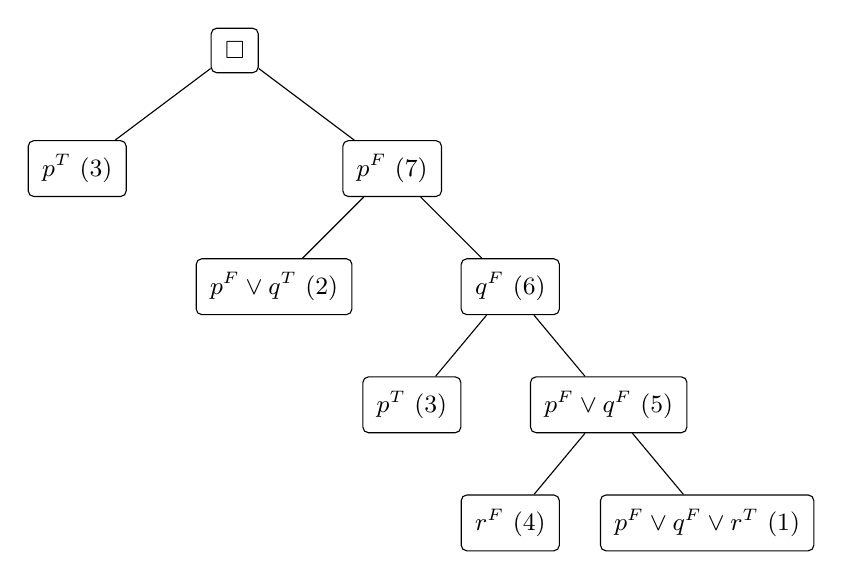
\begin{tikzpicture}[
  level distance=1.5cm,
  level 1/.style={sibling distance=4cm},
  level 2/.style={sibling distance=3cm},
  level 3/.style={sibling distance=2.5cm},
  edge from parent/.style={draw, thin},
  every node/.style={
    draw, 
    rectangle, 
    rounded corners=2pt, 
    inner sep=5pt, 
    font=\small
  }
]  
\node {$\square$}
  child {node {$p^T$ (3)}}
  child {node {$p^F$ (7)}
    child {node {$p^F \lor q^T$ (2)}}
    child {node {$q^F$ (6)}
      child {node {$p^T$ (3)}}
      child {node {$p^F \lor q^F$ (5)}
        child {node {$r^F$ (4)}}
        child {node {$p^F \lor q^F \lor r^T$ (1)}}
      }
    }
  };

\end{tikzpicture}    
\end{tcolorbox}
\caption{Resolution Proof Tree}
\label{fig:r0_proof_tree}
\end{figure}

\begin{example}[Resolution Given a Knowledge Base]{}
Consider we have a knowledge base $\text{KB} := \set{A \Rightarrow B \lor C , A, \neg B}$, we want to check if $\text{KB} \vDash C$. $\text{KB} \vDash C$ iff $\text{KB} \cup \set{\neg C}$ is unsatisfiable.

First we need to compute $\text{CNF} (A \Rightarrow B \lor C)$
\begin{itemize}
    \item $\text{CNF} (A \Rightarrow B \lor C) = \neg A \lor B \lor C$
\end{itemize}
$\text{KB} \cup \set{\neg C} := \set{\neg A \lor B \lor C, A, \neg B, \neg C} := \set{A^F \lor B^T \lor C^T, A^T, B^F, C^F}$

\begin{figure}[H]
\begin{tcolorbox}[colback=white, colframe=black, sharp corners, boxrule=0.5pt]
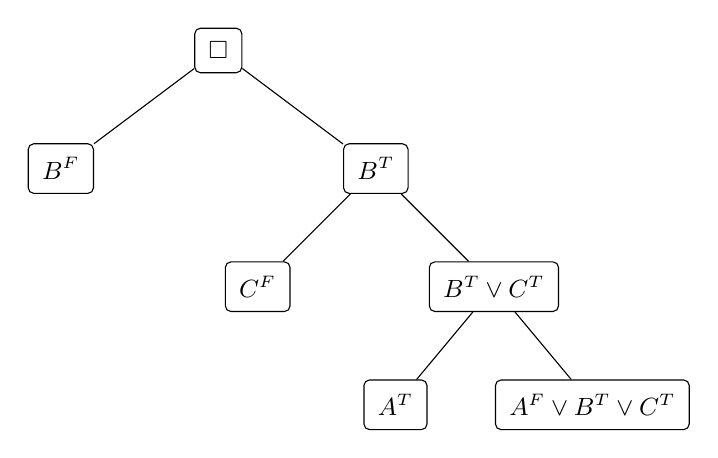
\begin{tikzpicture}[
  level distance=1.5cm,
  level 1/.style={sibling distance=4cm},
  level 2/.style={sibling distance=3cm},
  level 3/.style={sibling distance=2.5cm},
  edge from parent/.style={draw, thin},
  every node/.style={
    draw, 
    rectangle, 
    rounded corners=2pt, 
    inner sep=5pt, 
    font=\small
  }
]  
\node {$\square$}
  child {node {$B^F$}}
  child {node {$B^T$}
    child {node {$C^F$}}
    child {node {$B^T \lor C^T$}
      child {node {$A^T$}}
      child {node {$A^F \lor B^T \lor C^T$}
      }
    }
  };

\end{tikzpicture}  
\hfill
Since $\text{KB} \cup \set{\neg C}$ is unsatisfiable, $\text{KB} \vDash C$
\end{tcolorbox}
\end{figure}
\end{example}



\definition[Refutational Completeness]{
A test calculus $\mathcal{C}$ is called \textbf{refutationally complete} iff for every unsatisfiable clause set $\Phi$, there exists a refutation deriving the empty clause:
\[
\Phi \text{ is unsatisfiable} \iff \Phi \vdash_{\mathcal{C}} \square
\]
}{refutational_completeness}

\titledbox{Deductive vs. Refutational Completeness}{
Resolution is \textbf{not} deductively complete: from the clause set $\{p\}$, resolution cannot directly derive the valid consequence $p \lor q$. However, resolution is \textbf{sound and refutationally complete}: if we add the negation $\neg(p \lor q) \equiv p^F \land q^F$ to $\{p^T\}$, resolution is guaranteed to derive the contradiction $\square$.
}

\subsection{Horn Logic and SLD-Resolution}
\definition{
A \textbf{Horn clause} is a clause with \textbf{at most} one \textbf{positive} literal
}{}

\observationbox{
\begin{itemize}
    \item A rule in Prolog $H :- B_1, \dots, B_n$ corresponds to $H^T \lor B_1^F \lor \dots \lor B_n^F$, i.e. a Horn clause
    \item A goal set (query) $?- G_1, \dots, G_n$ asks for $G_1 \land \dots \land G_n$, which by refutation negates to the clause $G_1^F \lor \dots \lor G_n^F$
    \item A fact $F$ corresponds to the unit clause $F^T$
\end{itemize}
}

\definition[Horn Logic]{
Let $S := \langle \mathcal{L}, \mathcal{M}, \vDash \rangle$ be a logical system. A formal system $\langle S, \mathcal{C} \rangle$ is called a \textbf{Horn Logic} if:
\begin{itemize}
    \item The language $\mathcal{L}$ is the set of Horn clauses.
    \item The calculus $\mathcal{H}$ is defined by the rules of Modus Ponens ($\text{MP}$), Conjunction Introduction ($\land I$), and Substitution ($\texttt{Subst}$).
\end{itemize}
}{}


\definition[SLD-Resolution]{
\defemph{SLD-Resolution} (\textbf{S}elected literal, \textbf{L}inear resolution for \textbf{D}efinite clauses) is the formal inference calculus that executes Prolog programs. 

Conceptually, Prolog treats a query $\leftarrow A_1, A_2, \dots, A_k$ (in Prolog syntax: \texttt{?- A1, A2, ..., Ak}) as a \textbf{list of subgoals} that must all be satisfied:

At each execution step:
\begin{enumerate}
    \item \textbf{Selection:} Prolog picks the leftmost subgoal $A_1$ from the list.
    \item \textbf{Clause Lookup \& Unification:} Prolog searches the program for a clause $H \leftarrow B_1, \dots, B_m$ (whose variables are renamed to avoid name clashes) such that $A_1$ and the clause head $H$ unify with MGU $\sigma = \text{MGU}(A_1, H)$.
    \item \textbf{Goal Reduction (Replacement):} The subgoal $A_1$ is discharged and \textbf{replaced} by the requirements $B_1, \dots, B_m$ from the clause body. The substitution $\sigma$ is applied across the entire new goal list:
    \[
    \leftarrow \sigma(B_1, \dots, B_m, \; A_2, \dots, A_k)
    \]
    \textit{(If $H$ is a simple fact with no body, $A_1$ is removed without introducing new subgoals).}
\end{enumerate}
This reduction repeats until the goal list is completely empty ($\leftarrow \square$), which is called an \textbf{SLD-refutation}. The composition of all unifying substitutions $\sigma$ collected along the derivation forms the \textbf{answer substitution}.
}{sld_resolution}

\titledbox{The Name Behind the Acronym}{
\begin{itemize}
    \item \textbf{S (Selected literal):} Instead of searching randomly, Prolog uses a fixed selection rule: always pick the \textbf{first (leftmost)} subgoal.
    \item \textbf{L (Linear):} Every step is linear: it always resolves the \textbf{current query} against an input clause from the program; it never wastes time resolving two rules against each other.
    \item \textbf{D (Definite clauses):} The program is restricted to definite Horn clauses (each clause has exactly one head literal).
\end{itemize}
}


\definition[Answer Substitution]{
Let $P$ be a logic program (set of Horn clauses) and $Q$ a query. A substitution $\sigma$ is called an \textbf{answer substitution} for $Q$ if:
\begin{itemize}
    \item \textbf{Proof-theoretically:} There is a derivation $D$ of $Q$ from $P$, where $\sigma$ is the composition of all \texttt{Subst} instances in $D$.
    \item \textbf{Operationally:} There is an SLD-refutation of $P \cup \{\leftarrow Q\}$ with sequence of MGUs $\theta_1, \dots, \theta_n$, such that $\sigma = (\theta_1 \circ \dots \circ \theta_n)$ restricted to the variables of $Q$.
\end{itemize}
}{answer_substitution}

\begin{example}[Answer Substitution]{}
Consider the following program:
\begin{codeblock}
human(leibniz).
human(socrates).
greek(socrates).
fallible(X):-human(X).
\end{codeblock}

Where we query \inlinecode{?-fallible(X), greek(X).}

We have three facts, one rule, and one query. They translate to the following clause set:
\begin{enumerate}
    \item $\text{human(leibniz)}^T$
    \item $\text{human(socrates)}^T$
    \item $\text{greek(socrates)}^T$
    \item $\text{fallible}(X)^T \lor \text{human}(X)^F$ \hfill ($\text{human}(X) \Rightarrow \text{fallible}(X)$)
    \item $\text{fallible}(X)^F \lor \text{greek}(X)^F$ \hfill (Start Resolution)
    \item Resolve (1) with (4) under $[\text{leibniz} / X] \leadsto \text{fallible}(\text{leibniz})^T$
    \item Resolve (5) with (6) under $[\text{leibniz} / X] \leadsto \text{greek}(\text{leibniz})^F$
    \item $\text{greek}(\text{leibniz})^F$ cannot be resolved further; the program backtracks to try another substitution.
    \item Resolve (2) with (4) under $[\text{socrates} / X] \leadsto \text{fallible}(\text{socrates})^T$
    \item Resolve (5) with (9) under $[\text{socrates} / X] \leadsto \text{greek}(\text{socrates})^F$
    \item Resolve (3) with (10) $\leadsto \{ \square \}$
    \item The program returns $T$ and the answer substitution $\sigma := [\text{socrates} / X]$.
\end{enumerate}
\end{example}

\commandnote{
Prolog's query engine natively executes backchaining (SLD-resolution). However, from a proof-theoretic standpoint, the exact same Horn knowledge base can also establish truths via forward chaining!
}

\titledbox{Forward Chaining}{
A bottom-up, data-driven derivation that starts with known facts and repeatedly applies program rules (via Modus Ponens and substitution) to infer new facts until the desired conclusion is produced.
}

\begin{example}[Backchaining]{}
Consider the program:
\begin{codeblock}
has_motor(c).
has_wheels(c,4).
car(X) :- has_motor(X), has_wheels(X,4).
\end{codeblock}   

And the query \inlinecode{?-car(X).}

We have two facts, one rule, and one query. They translate to the following clause set:
\begin{enumerate}
    \item $\text{m}(c)^T$
    \item $\text{w}(c,4)^T$
    \item $\text{c}(X)^T \lor \text{m}(X)^F \lor \text{w}(X,4)^F$ \hfill ($\text{m}(X) \land \text{w}(X,4) \Rightarrow \text{c}(X)$)
    \item $\text{c}(X)^F$ \hfill (Start Resolution)
    \item Resolve (3) with (4) $\leadsto \text{m}(X)^F \lor \text{w}(X,4)^F$ 
    \item Resolve (5) with (1) under $[c / X] \leadsto \text{w}(c,4)^F$
    \item Resolve (6) with (2) $\leadsto \{ \square \}$
    \item The program returns $T$ and the answer substitution $\sigma := [c / X]$.
\end{enumerate}
\end{example}

\begin{example}[Forward Chaining in Horn Logic]{ex:forward_chaining}
Consider the same program. Instead of Prolog's top-down query execution, we examine how the formal calculus of Horn Logic $\mathcal{H}$ derives truths \textbf{forward} (bottom-up) from the program's clauses taken as axioms:
\begin{enumerate}
    \item $m(c)$
    \item $w(c,4)$
    \item $m(X) \land w(X,4) \Rightarrow \text{car}(X)$
\end{enumerate}   

Using the inference rules of Horn logic, the logical consequence $\text{car}(c)$ is derived as follows:

\[
\infer[MP]{\text{car}(c)}{
    \infer[\land I]{m(c) \land w(c,4)}{
        \infer[Ax]{m(c)}{}
        &
        \infer[Ax]{w(c,4)}{}
    }
    &
    \infer[\text{Subst [c/X]}]{m(c) \land w(c,4) \Rightarrow car(c)}{
        \infer[Ax]{m(X) \land w(X,4) \Rightarrow car(X)}{}
    }
}
\]
\end{example}

\titledbox{Conclusion}{
\begin{itemize}
    \item \textbf{Forward Chaining:} A bottom-up derivation in $\mathcal{H}$ starts from the axioms and builds up to the conclusion $\text{car}(c)$.
    \item \textbf{Backward Chaining:} Prolog starts with the query $\leftarrow \text{car}(X)$ and uses SLD-refutation to reduce goals top-down to $\square$, computing the exact same answer substitution $\sigma = [c/X]$.
\end{itemize}
}

\nocite{*}
\printbibliography
\end{document}
